% Author: Matej Otcenas
%%%%%%%%%%%%%%%%%%%%%%%%%%%%%%%%%%%%%%%%%%%%%%%%%%%%%%%%%%%%%%%%%%%%%%%%%%%%%%%%%%%%%%%%%%%%%%%%%%%%%%%%%%%%
\chapter{Introduction}
Nowadays, besides studying medical literature or performing long X-ray observations, there are other possible ways to carry out a detailed analysis of the human body to identify diseases. Thanks to technical progress it is possible to apply a wide range of algorithms, which can detect a variety of arising diseases not even a human eye can recognize.

Various organ disorders can be detected through application of these technical methods, such as examining lung X-ray to diagnose pneumonia, brain screens to brain tumour detection or metacarpal bones investigation to detect early stage of rheumatic disease. If we could prevent earlier such diseases we would be able to avoid more fatalities every day. One~of~the major parts in this segment is digital image processing.

This thesis describes the digital image processing to detect the contours of the metacarpal bones in the human hand which circumference is then measured. Such an approach aims to create a final program with an output database of measurement values which will serve the Faculty of Science of Masaryk University(MUNI) for detailed analysis thanks to which they avoid manual measurements, which can lead to inaccuracies caused by human error. This approach will ensure more accurate and effective evaluations of outcomes that monitor various adverse growth factors or detect genetic disorders.

To obtain such measurements, it is necessary to detect the individual edges of the bones as~accurately as possible. However, this approach has to deal with several problems, such~as~the~overlapping of individual metacarpal bones or the nonuniformity of the X-ray images.

Traditional image processing itself, consists of several steps. First, the image is loaded and the possible noise reduction is performed, which can be done using various filters, which will blur the image as a result. This is followed by image contrast enhancement and image segmentation, which separates the foreground from the background using the right algorithm technique. At last the edges of desired object can be detected with the following contour detection if needed.

However, this approach can often be insufficient and inaccurate when it comes to more complex extraction of objects in the image. The most serious problem can arise in image segmentation, where we try to extract a relatively unusual specific shape. This shape can be, for example, a kind of irregular polygon, which can be covered in the picture by many different but also similar shapes, which, however, are not the subject of research. Thus,~if~one of the options presented, traditional methods for a larger amount of tested data begin to fail. 

In such case, it can be better achieved by relatively more complicated, but more accurate methods for processing and segmenting the medical image, such as neural networks, more specifically convolutional neural networks(CNN). 

\section{Aim of the Thesis} 
This work aims to design and implement an algorithm that detects the contour of third metacarpal bone in the human hand from X-ray images and measure its circumference at the narrowest part. The thesis focuses on creating an algorithm to automate measurements on~X-rays, which are provided by the Faculty of Science MUNI so that there is no need to measure and click points manually and to reduce the deviations that can arise as a human factor failure.

\section{Contents}
The chapter \ref{state-of-the-art} focuses on the anatomy of the human hand itself, which is essential for~a~closer understanding of the problem of metacarpal bones detection. The chapter also describes current traditional image processing methods for pattern recognition using image segmentation and edge detection that can be used for X-ray images. Despite the usability of~such methods, the chapter describes the possibilities of using deep learning with CNN, which are now very popular in segmenting the image and pulling a specific mask from the image. Chapter \ref{chapter3} describes a specific design of an algorithm for image segmentation of the bone using basic image preprocessing methods and their effects on the images. The~section \ref{cnn-design} in this chapter focuses on the use of convolutional neural networks, which appear to be more reliable in~obtaining a mask for the third metacarpal bone, which does not require image preprocessing and also describes a proposal for analytical measurement of bone in its narrowest part. Furthermore, chapter explains the use of traditional methods in image processing in combination with CNN, such as Canny edge detector. On~the~basis~of~continuous communication with the anthropological institute, the section \ref{extenstion-design} describes~a~specific extension of algorithm, which is able to measure the individual narrowest parts~of~the bone in three separate regions. The bone structure itself is introduced in the section \ref{tmb-structure}, which describes in detail what parts of the bone is talked about. The section \ref{implementation} is focused on the~proposed design, implementation and usage of an algorithm. The chapter \ref{testing} focuses on the testing~of~the~program that was created on the given available database of~manual measurements provided by the~Faculty of Science MUNI. The chapter also focuses on hardware resources and possible speed optimization because of the~complexity and computational difficulty of the~algorithm. At last, the chapter \ref{conclusion} summarizes this thesis and discusses the~possible extensions and improvements for the created algorithm.

%%%%%%%%%%%%%%%%%%%%%%%%%%%%%%%%%%%%%%%%%%%%%%%%%%%%%%%%%%%%%%%%%%%%%%%%%%%%%%%%%%%%%%%%%%%%%%%%%%%%%%%%%%%%
\chapter{State of the Art}
\label{state-of-the-art}

\section{Human Hand Anatomy}
Human hand is composed of number of bones, that are shown on image \ref{bones} of which every single one has its own purpose. Very important part of bone examination is reveal of genetic and growth disorders, which can be detected directly by observation of inner hand bones, for example metacarpal bones. This approach enables revelation of Turner's syndrome, dyschondrosteosis or hypochondroplasia \cite{diseases}. X-ray images show the natural deformation of the bone itself, which occurs more frequently with the aging of the organism. The~picture \ref{overlap-img} shows frequent overlapping of the bones \cite{bones-deformation}. On the contrary, children's bones as seen on the picture \ref{non-overlap-img} are predominantly separated from each other and do not overlap, which offers an advantage and simplification for segmentation of the image and~detection~of~the~edges. This phenomenon is caused by the fact that the skeleton~in~children is mostly composed of cartilaginous bones, which contain only small amount of inorganic substances and minerals such as calcium and this results in lower density of the bones. Growing older, these bones start to change and soft cartilage ossifies, and therefore~the~bone~density grows bigger \cite{aging-effect}.

\begin{figure}[!ht]
  \centering
  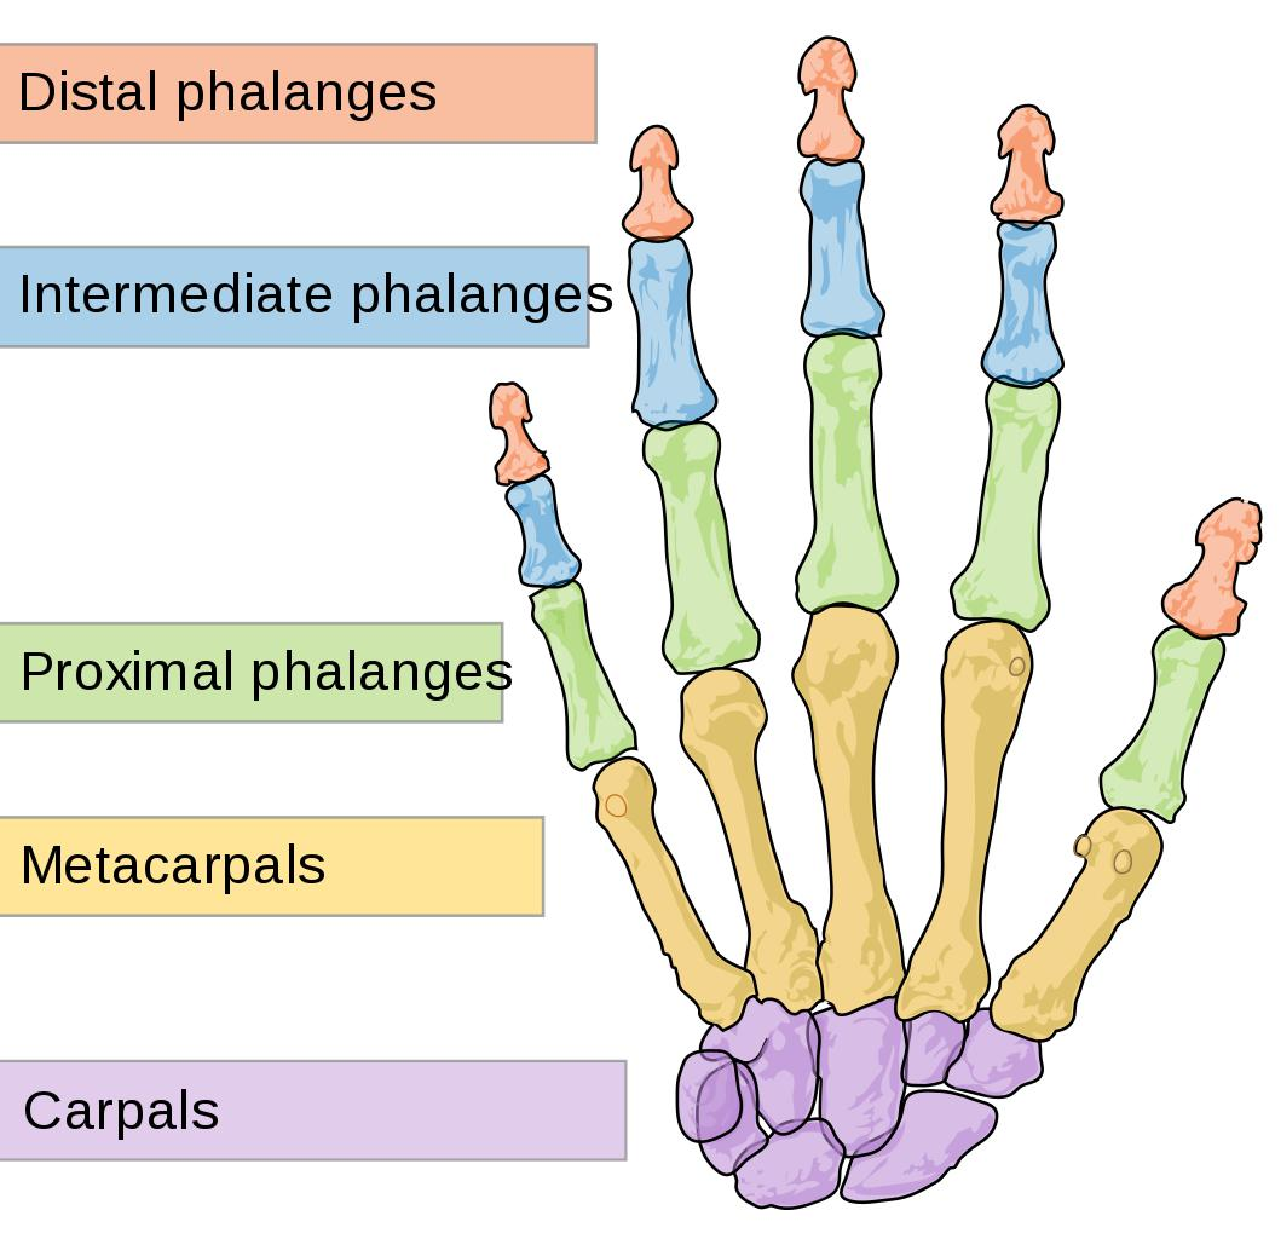
\includegraphics[width=.4\textwidth]{obrazky-figures/human_hand.pdf}
  \caption{\textbf{Human hand bones.} Main interest of the human hand bones in this work are the metacarpals shown as yellow bones in the image \cite{human-hand}.}
  \label{bones}
\end{figure}

\begin{figure}[!ht]
    \centering
    \begin{subfigure}[b]{.45\textwidth}
    \centering
        \frame{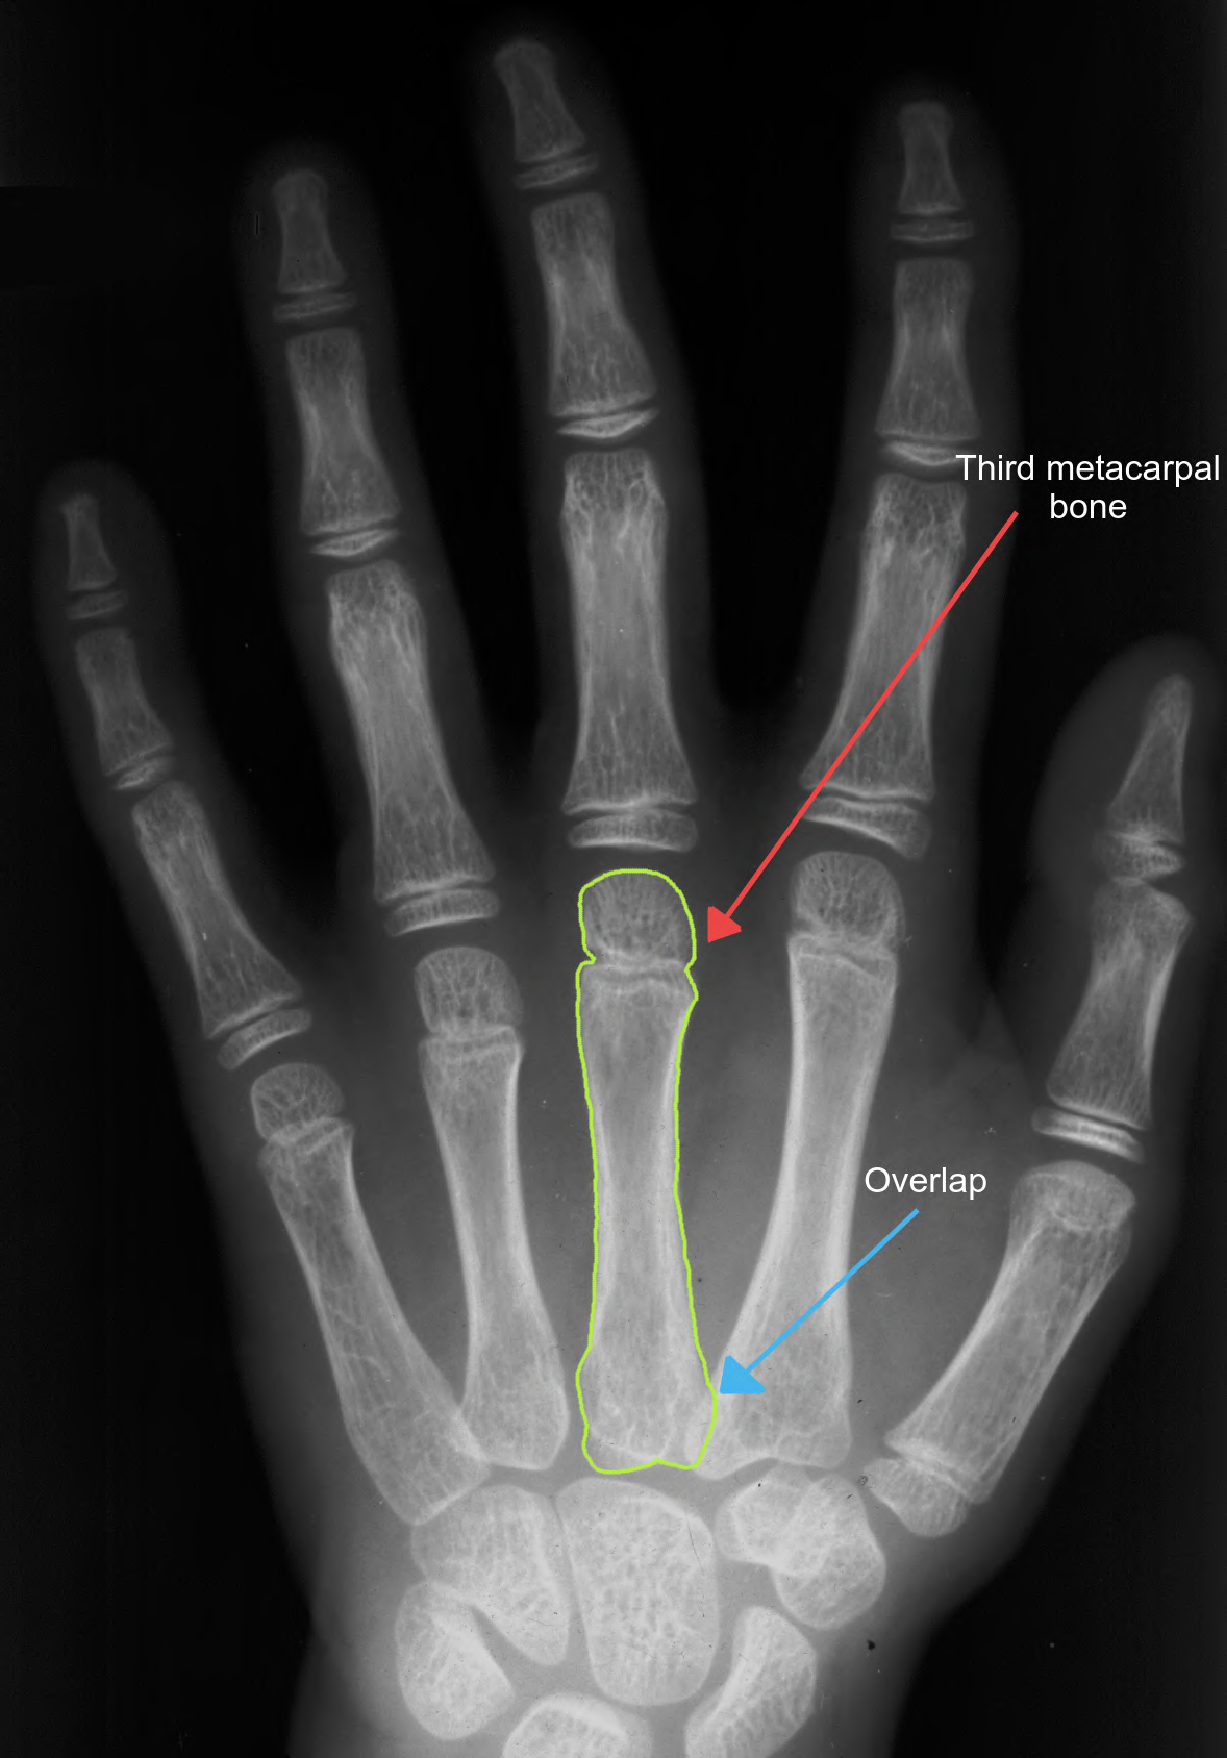
\includegraphics[width=.9\textwidth,height=3.58in]{obrazky-figures/metacarpal_bone.pdf}}
        \caption{}\label{overlap-img}
    \end{subfigure}
    \begin{subfigure}[b]{.45\textwidth}
    \centering
        \frame{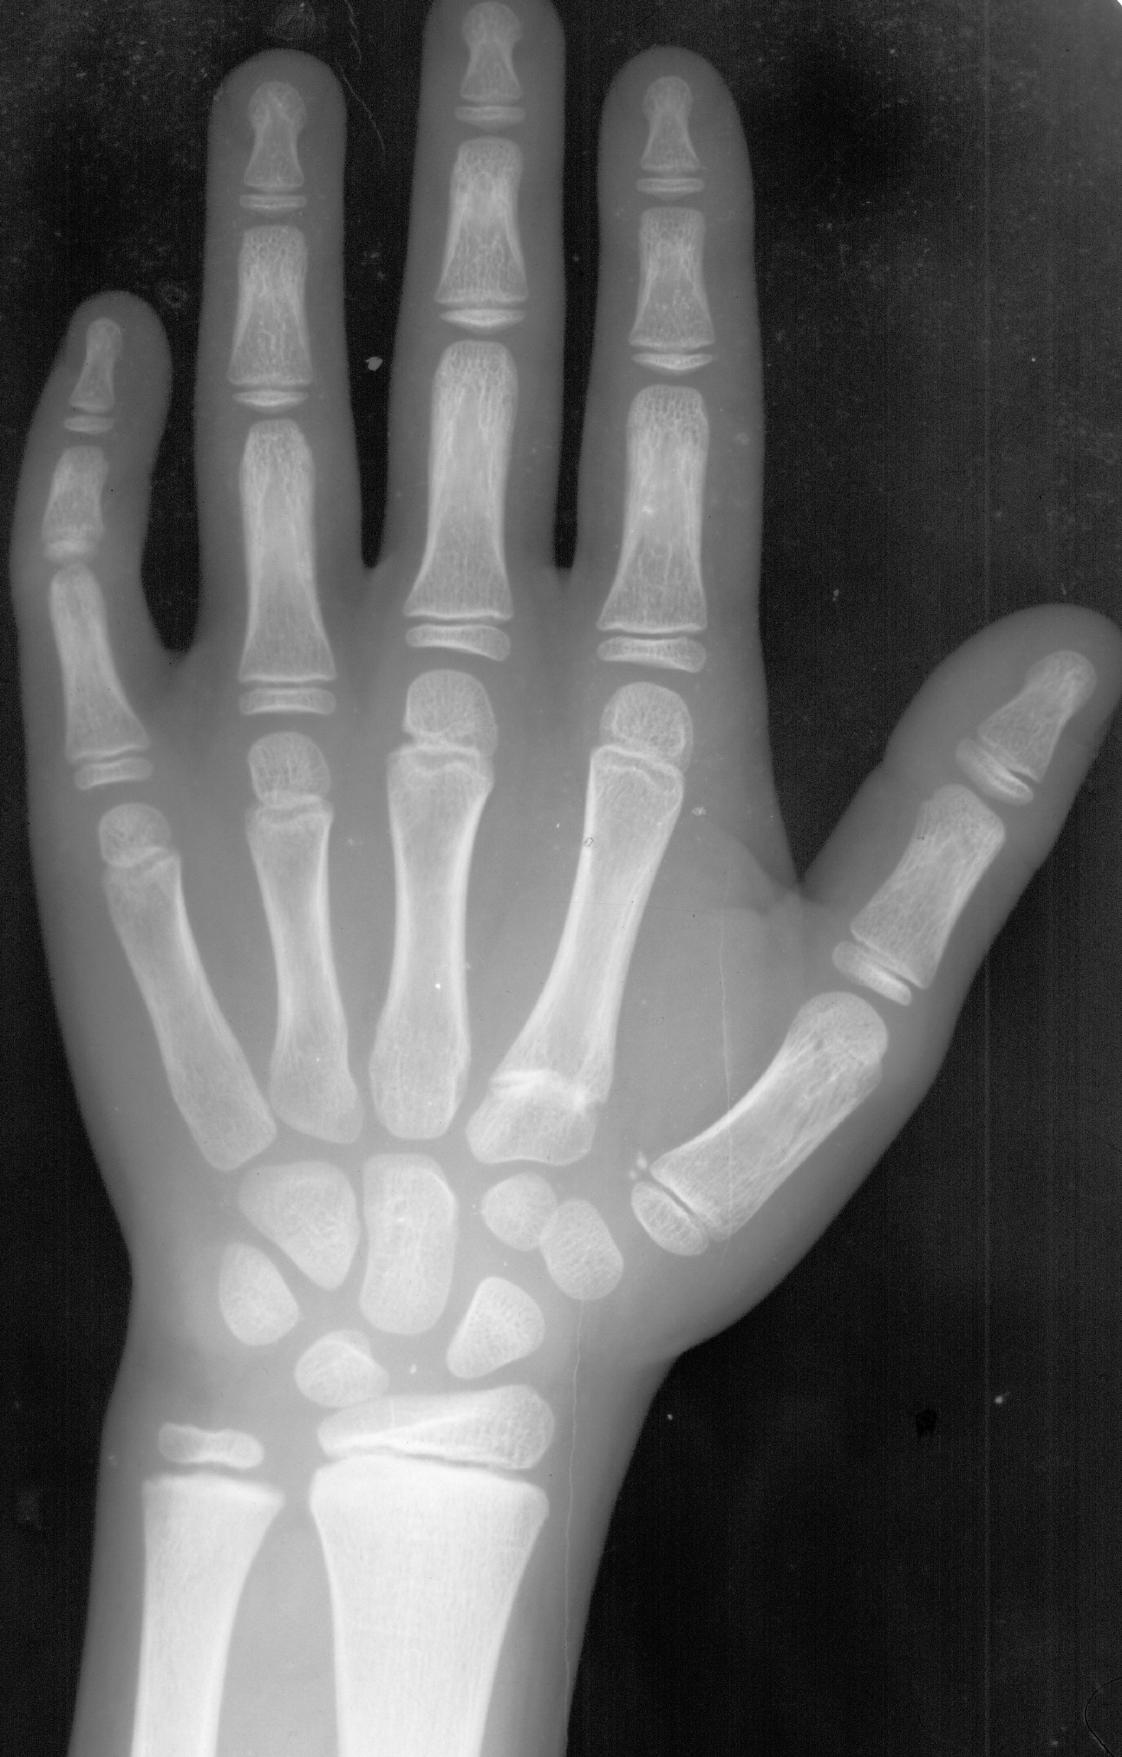
\includegraphics[width=.9\textwidth,height=3.58in]{obrazky-figures/child_metacarpal.pdf}}
        \caption{}\label{non-overlap-img}
    \end{subfigure}
    
    \caption{\textbf{X-ray images comparison.} (a) Hand of the grown up human showing~the~overlap of third metacarpal bone. (b) X-ray image of child human hand with no overlap.}
    \label{overlap-images}
\end{figure}

\section{Third Metacarpal Bone Structure}
\label{tmb-structure}
Each of the metacarpal bones has basic structure. In general, the bones of metacarpals are made up of three parts. The first is the \textit{base}, which forms the foundation of the bone, then the largest part is the \textit{body} or \textit{shaft} of the bone. Finally,~the~bone is finished with~the~so-called \textit{head} of the bone as shown in the picture \ref{head-base-body} \cite{metacarpal-structure-radiopedia}. The head and base~of~the~bone are also medically called \textit{epiphyses}. The body of the bone is professionally called \textit{diaphysis}, which is the most important part of measuring bone width. From~the~radiological point~of~view, it is very important to describe the physical structure of the bone. It consists primarily~of~two specific parts, which are color-coded on the X-ray image. These parts are \textit{compact bones} and \textit{medullary cavity}. The image \ref{long-bone-structure} shows in more detail what part~of~the~bone~it is. If we work with~the~X-ray image shown on picture \ref{zoomed-3meta-img}, the compact bone has a light color and is located on the edges of the bone. Contrariwise, the medullary cavity is significantly darker. In regard to image processing, the bone can be divided into three separate regions shown on image \ref{zoomed-3meta-3segments-img}.

\begin{figure}[!ht]
    \centering
    \begin{subfigure}[b]{.40\textwidth}
    \centering
        \frame{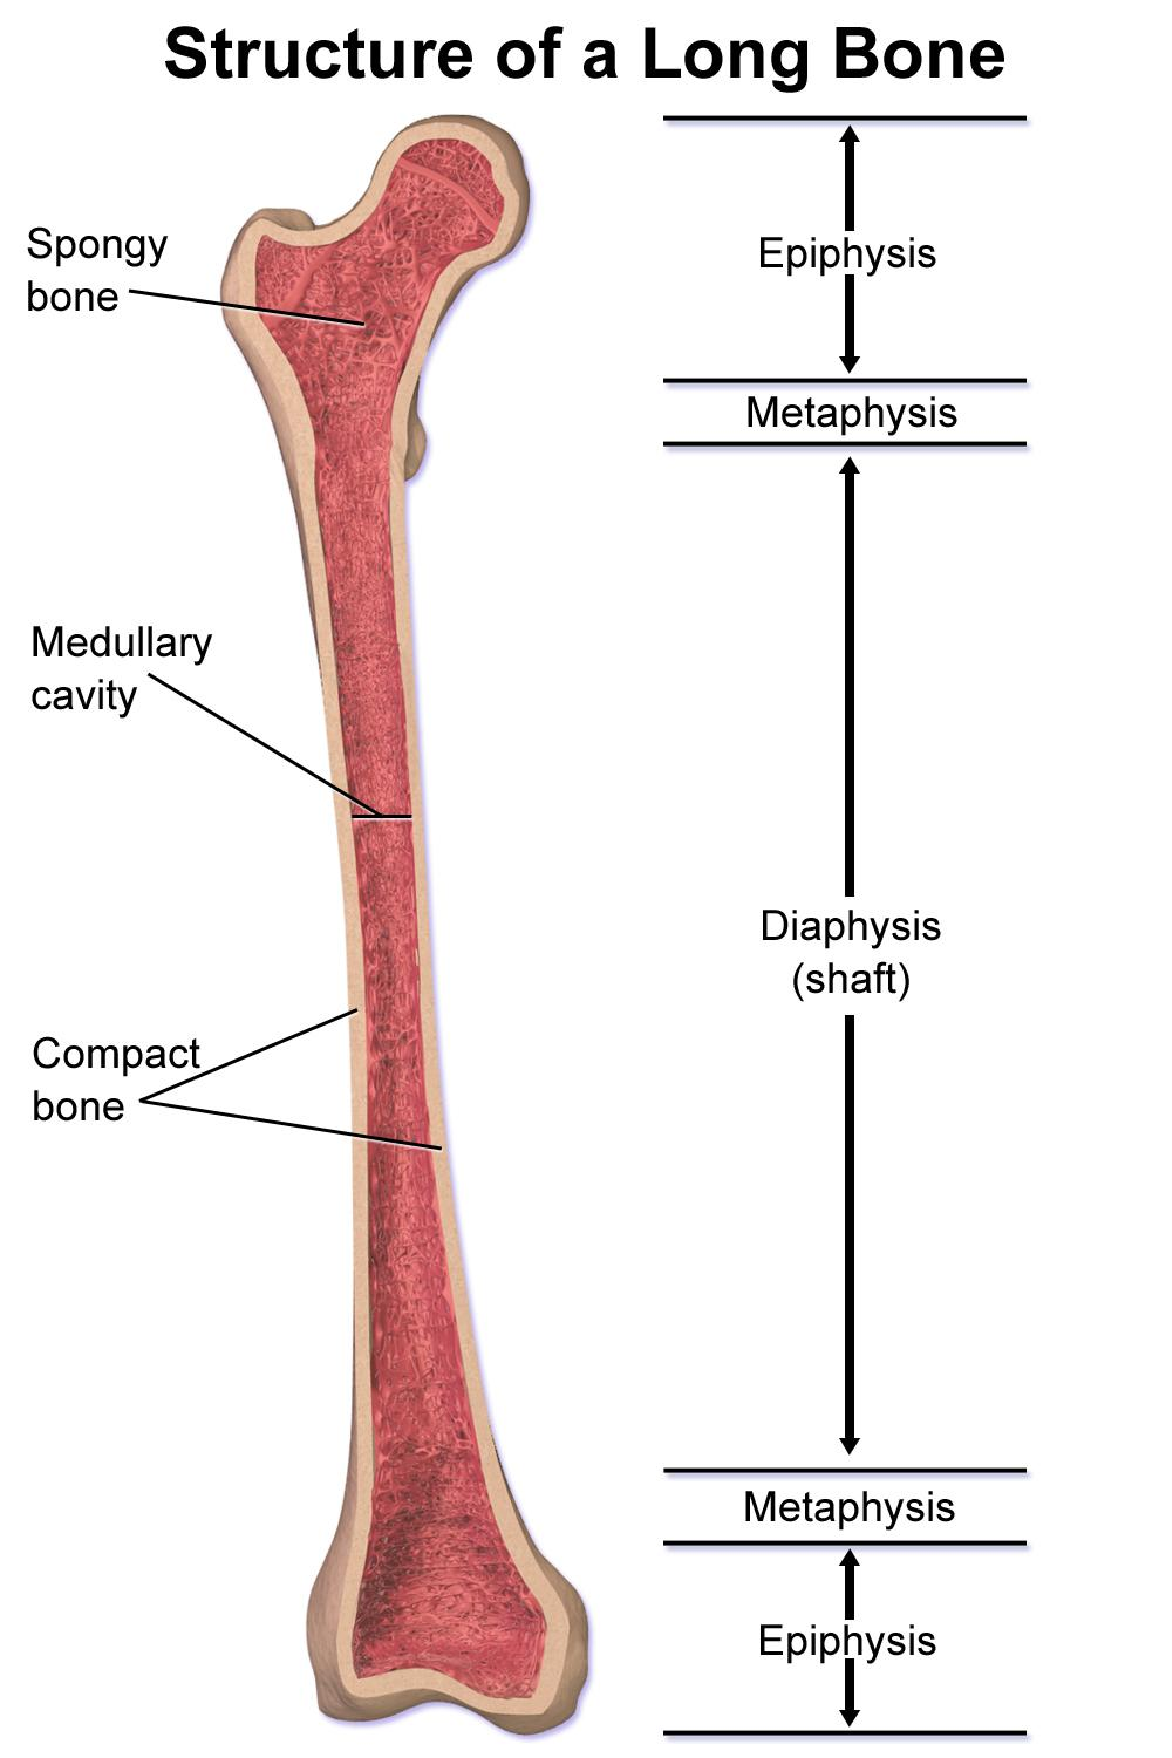
\includegraphics[width=\textwidth]{obrazky-figures/Structure_of_a_Long_Bone.pdf}}
        \caption{}\label{long-bone-structure}
    \end{subfigure}
    \hspace{1cm}
    \begin{subfigure}[b]{.40\textwidth}
    \centering
        \frame{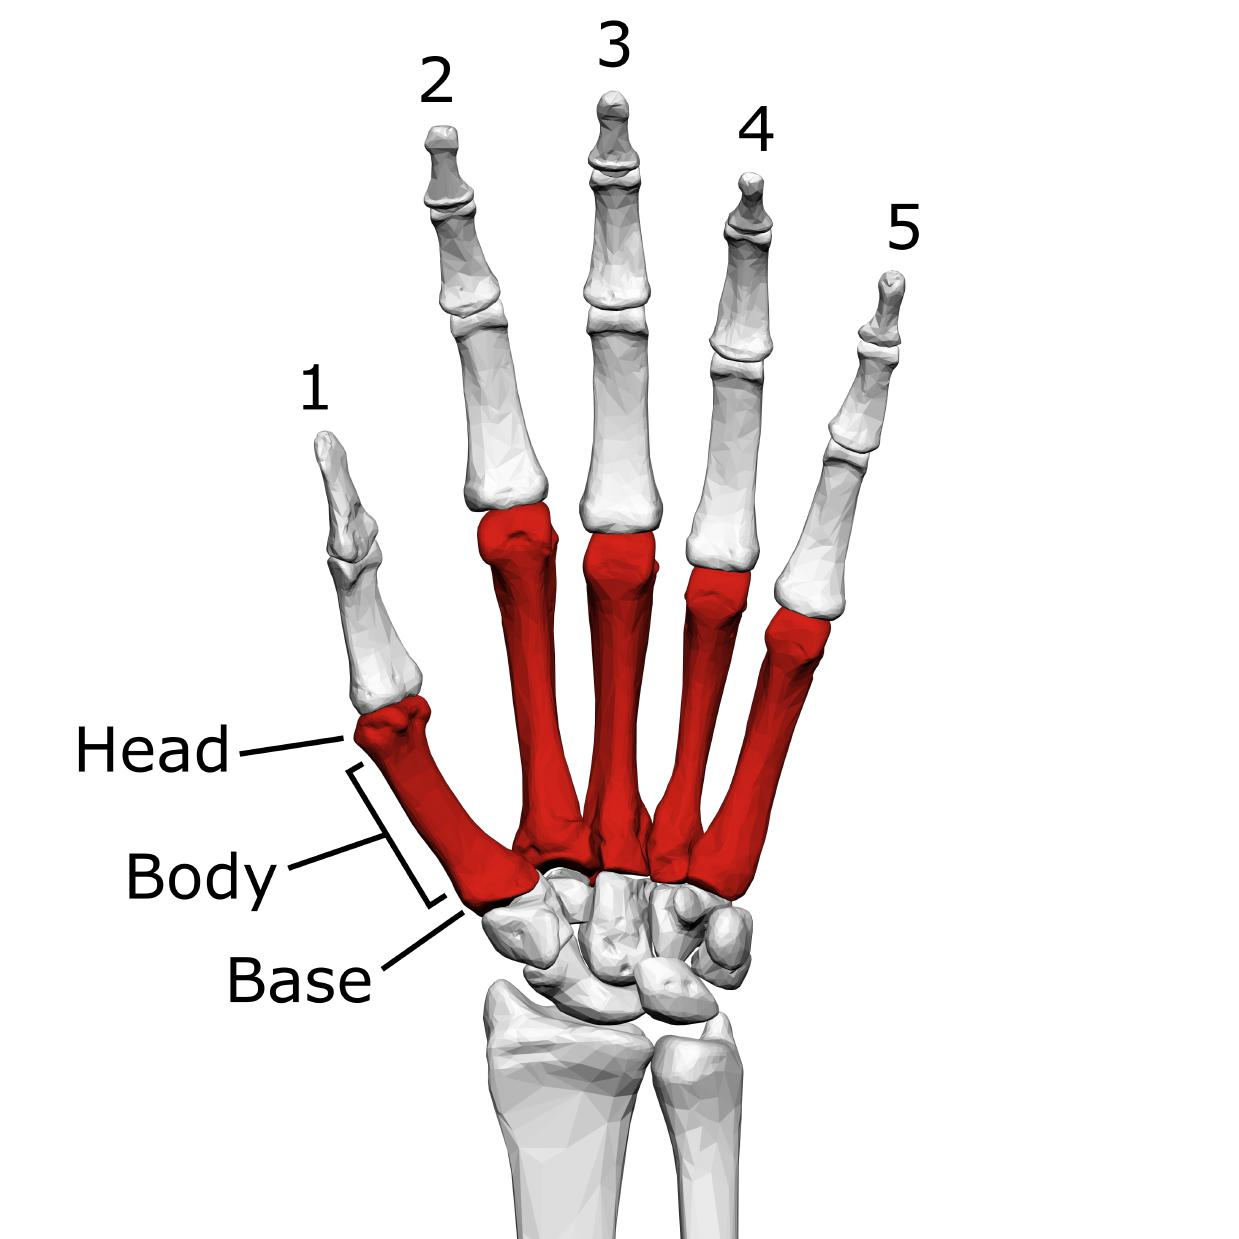
\includegraphics[width=\textwidth,height=3.59in]{obrazky-figures/Metacarpal_bones_(left_hand)_01_palmar_view_with_label.pdf}}
        \caption{}\label{head-base-body}
    \end{subfigure}
    
    \begin{subfigure}[b]{.35\textwidth}
    \centering
        \frame{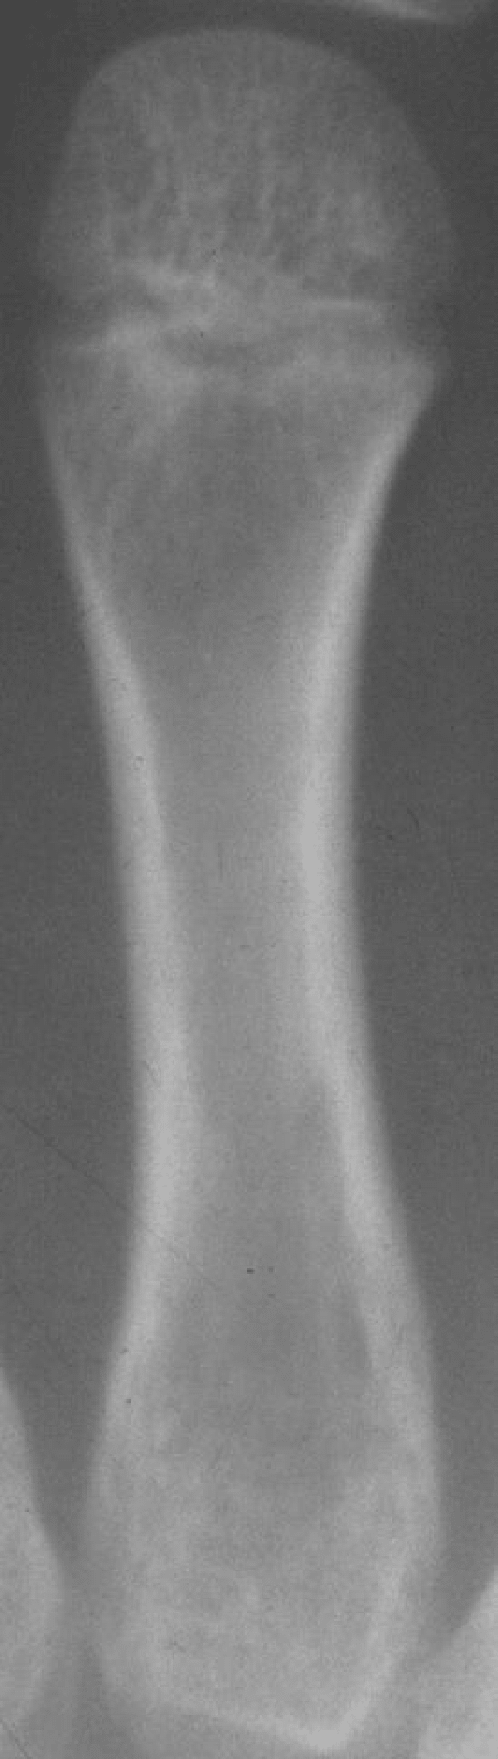
\includegraphics[width=.8\textwidth,height=3in]{obrazky-figures/3metacarpal-zoomed-3segments.pdf}}
        \caption{}\label{zoomed-3meta-3segments-img}
    \end{subfigure}
    \hspace{1cm}
    \begin{subfigure}[b]{.35\textwidth}
    \centering
        \frame{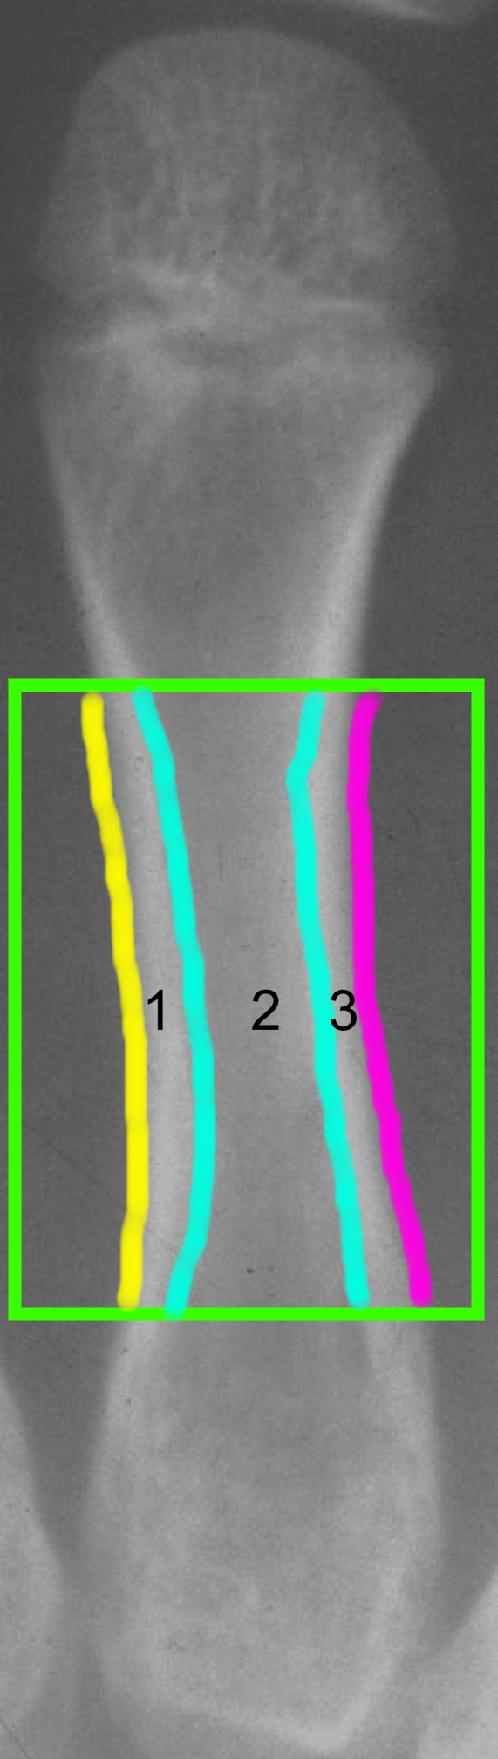
\includegraphics[width=.8\textwidth,height=3in]{obrazky-figures/3metacarpal-zoomed.pdf}}
        \caption{}\label{zoomed-3meta-img}
    \end{subfigure}
   
    \caption{\textbf{Third metacarpal bone structures.} (a) Medical view of long bone structure~\cite{wiki-long-bone}. (b)  Basic bone structure \cite{wiki-bone-structure}. (c) X-ray image of third metacarpal bone. (d) X-ray image showing three individual segments.}
    \label{xray-images}
\end{figure}

\section{Radiography}
Radiography is a method for creating image throughout X-ray pictures and gamma emission to visualize inner body parts. This procedure is mainly used in medicine or anthropology and is usually connected with bone diagnostics \cite{radiography}.

\subsection{X-ray Image}
X-ray images are produced due to electromagnetic radiation, which is absorbed in~the~individual parts of the body. X-rays travel through~the~body and are absorbed in different amounts~by~tissues possessing different radiological density, having strong impact~on~the~final formation~of~the X-ray image. If~the~density~of~the displayed organ is low, its brightness is significantly lower and the object appears darker~in~the~final image. On the other hand, if~the~displayed tissue's density is bigger~,~the~final image seems brighter and its color resembles white. Roentgen images of the bones and their eventual brightness is influenced for example by the amount of calcium in the bones – the bigger the amount~of~calcium~,~the~lighter~the~shade of the displayed bone \cite{x-ray, x-ray-colors}.

\section{Digital Image}
It is possible to imagine a digital image as a \textit{\say{function f(x,y) of two continuous variables x and y}} \cite{image-processing-intro3}. In order to be able to process this image digitally, it must be sampled and transformed into a numerical matrix, which in the end represents a three-dimensional image where the third dimension stands for proportion of colors in colored image or the~amount of light in grayscale image. This image is then composed of items called pixels. In the most common way the pixels are sorted into the rectangular shape using the pixel coordinate system where the \textit{y-axis} is vertically flipped. Image \ref{digital-img} shows the layout of digital image with better understanding of the coordinate system. The image width represents the actual number of columns, and at the same time the image height is the number of rows.  Number~of~pixels can be defined as $ Pixels = M \times N $, where \textit{M} is the number of rows and \textit{N} is the number of columns \cite{image-processing-intro4}.
\begin{figure}[ht]
  \centering
  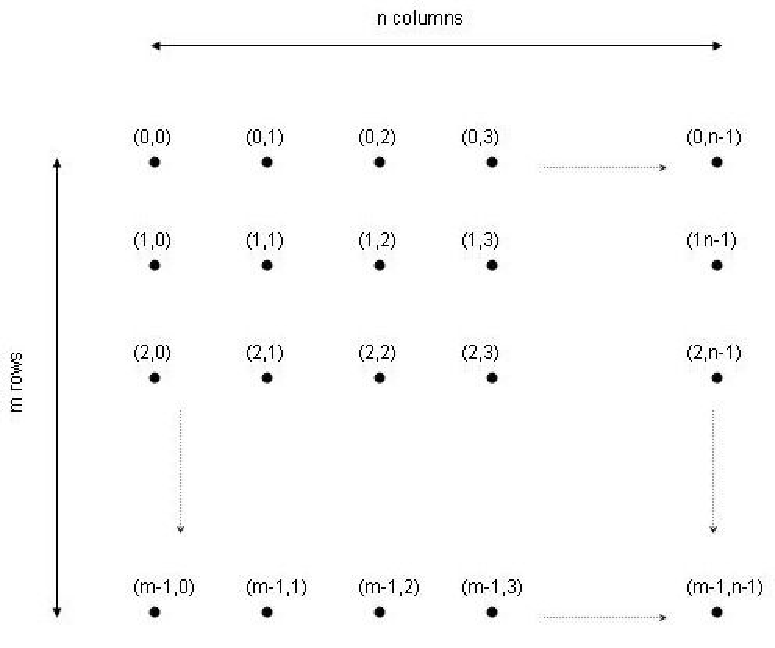
\includegraphics[width=.66\textwidth]{obrazky-figures/digtal-img-imatrix.pdf}
  \caption{\textbf{Digital image layout.} The image depicts how the individual pixel coordinates are perceived in the digital images coordinate system \cite{digital-img}.}
  \label{digital-img}
\end{figure}

\section{Human Hand Digital Image Processing}
Image processing is very important and rather difficult task always including a number of~essential steps. Application and use of this discipline is broad and is encountered on daily basis for instance in modern systems for object recognition in car ride, facial recognition to~unlock the phone, in photo and picture editors to improve their quality and last but not least, in analysis of medical images, such as X-ray images to reveal diverse anomalies and disorders \cite{image-processing-intro, image-processing-intro2}. Digital image of~medical pictures may originate from various sources, of~which every one uses different technique for its performance, namely magnetic resonance imagining or computer tomography. Their area of interest are various body parts and body structures such as soft tissues or bones, amongst which especially the bones are most frequently examined using X-radiation and are also the major subject of~this thesis, specifically the processing of digital X-ray images.

\section{Traditional Image Processing Methods}

\subsection{Grayscaling}
One of the introductory and fundamental steps of preprocessing of the image is the conversion of the picture from the color channel to typically \textsc{256} values of gray~where~the~lowest value is \textsc{0}(black color) and~the~highest is \textsc{255}(white color). Digital image is usually composed of three color channels of which every channel presents one individual color. They mostly represent red, green and blue color(RGB) and every one~of~these channels contains luminance value to define the brightness~of~the~color. To~acquire grayscale image which will only~consist~of~the~levels~of~gray,~it~is necessary~to~remove all three~of~the~color channels leaving only the value~of~the luminance according to formula \cite{grayscale, grayscale-formula}:
\begin{equation}
Luminace = 0.299 * Red + 0.587 * Green + 0.114 * Blue 
\end{equation}
This process is of great importance for improvement of the image segmentation and edge detection, which would not be possible to reveal in colored pictures. It is a preferred approach in image analysis as it enables to omit the excess amount of information in form of color value and by doing so, simplifies computational process. In above mentioned methods, these information do not feature as valuable. 

In case of X-ray images, this step is not to be performed in any way due to the fact, that the final X-ray images in digital form are comprised solely of shades of grey color and ignore the color channels from its very essence. This is because the color in X-ray images is non-essential and in the same way it is not useful in the exposure of the disorders and anomalies we use roentgen imagining for.

\subsection{Noise Reduction}
% \begin{itemize}
%     \item Noise: It is an undesirable phenomenon which is made by the very formation~of~the~image, it disrupts the final appearance and complicates detailed analysis~of~the~image. The individual noise can be also defined as \textit{\say{random variation of brightness or color information in the images captured. It is degradation in image signal caused by external sources \cite{image-noise2}.}}
% \end{itemize}

Very important part of preprocessing of the image is smoothing, which is manifested by~removal of the noise from the digital image. The problem of a great noise is, that it can cause reduction of visibility of certain inspected parameters in the image, such as the edges of the bones in an X-ray image \cite{image-noise}. Due to this feature, it is necessary to use particular methods to remove the pre-formed noise, but yet be careful of undersegmentation caused by excessive
smoothing. Contrariwise, in case of unrestricted noise it will lead to reverse effect which is oversegmentation.

The removal of the noise may be performed using so called noise reduction filters, whose principle is based mainly in averaging ambient pixel values into one ultimate value. This~filter can be pictured as two dimensional matrix with appropriately chosen size, which is usually known under the name \textit{kernel} or \textit{mask} and contains values depending~on~the~type~of~selected filter, which is then enclosed~to~the~large two dimensional matrix~of~the image from the left to~the~right and from~the~top~to~the~bottom direction. The removal~of~the~noise may be performed using so called noise reduction filters, whose principle~is~based mainly~in~averaging ambient pixel values into one ultimate value \cite{image-noise3}.

There are several types of filters and they all differ in their properties regarding filtration of~the~image. One of the most popular filters is the so-called Gaussian filter, which is also used in the Canny edge detector method. Application of the~correct filter depends on~the~type of the~noise or on individual latter focus of image processing. Testing individual filters and comparing the quality of their results with regard to required properties of~subsequent analysis is extremely important. The effect of noise reduction can be seen on~images \ref{denoised}.

\begin{figure}[!ht]
    \centering
    \begin{subfigure}[b]{.45\textwidth}
    \centering
        \frame{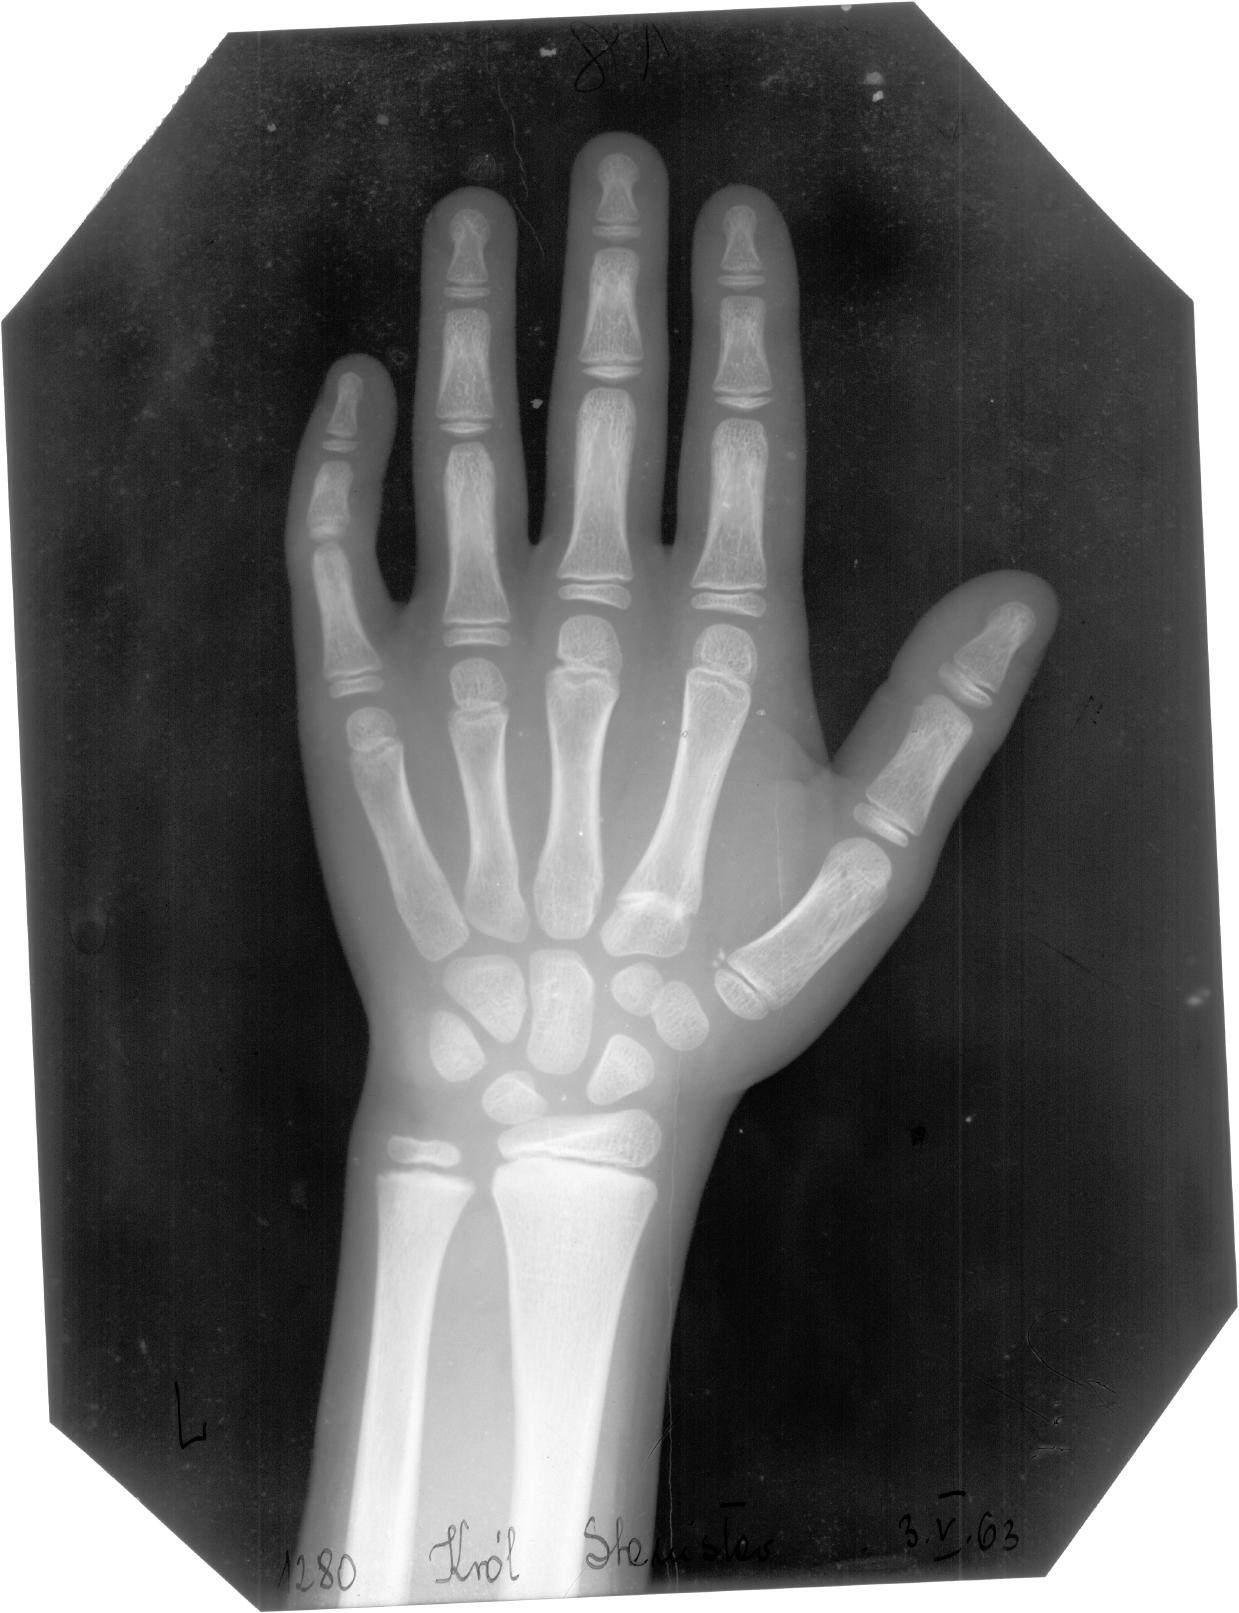
\includegraphics[width=.75\textwidth]{obrazky-figures/non-blurred.pdf}}
        \caption{}\label{classic-img}
    \end{subfigure}
    \begin{subfigure}[b]{.45\textwidth}
    \centering
        \frame{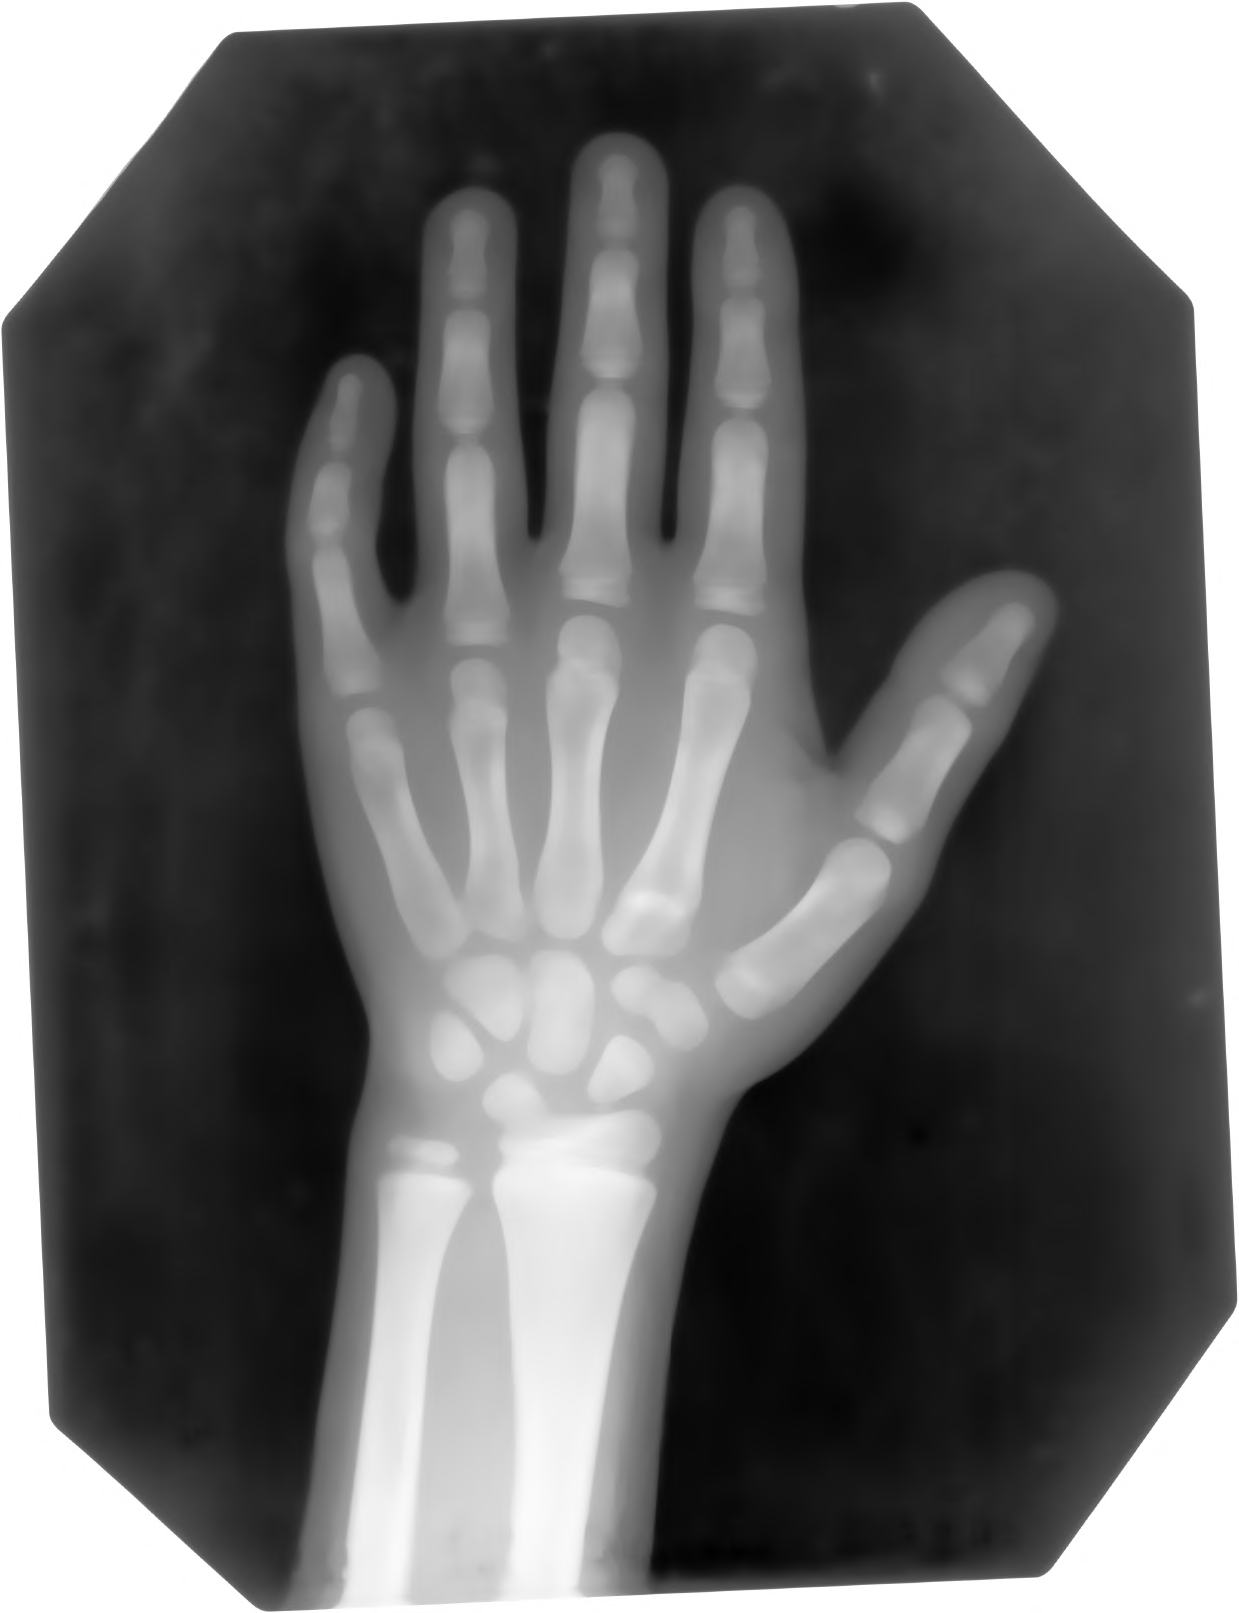
\includegraphics[width=.75\textwidth]{obrazky-figures/blurred.pdf}}
        \caption{}\label{denoised-img}
    \end{subfigure}
     \caption{\textbf{Denoising effect.} (a) Normal X-ray image. (b) Blurred X-ray image.}
    \label{denoised}
\end{figure}

\subsection{Thresholding}
\label{classic-thresh}
One of the basic algorithms used for image segmentation is thresholding. The output of~this algorithm is an image in binary form, which means it is containing only two colors and that is white with pixel value of 255 and black with value of 0 which can be seen in the pictures \ref{thresholds}. The basic thresholding function is defined by formula \ref{eq:threshold}.
\begin{equation}
    g(x,y)= 
\begin{dcases*}
    255 & \text{if } (x,y) > \textbf{T} \\
    0 & \text{otherwise}
\end{dcases*}
\label{eq:threshold}
\end{equation}   
Variable \textbf{T} is a suitable threshold.

If this classic threshold approach would be used on graphically~enhanced~image~from~the~X-ray~dataset, freed of noise, output shown on image \ref{classic-thresh-img} is quite unpleasant.

However, the thresholding method may have several other approaches for image segmentation, which are a bit more complicated but are able to segment the image with better accuracy. It can be segmented using the so-called Otsu's thresholding method described~in~the~section \ref{Otsu} or using the adaptive thresholding described in the section~\ref{Adaptive}.

\subsection{Adaptive Thresholding}
\label{Adaptive}
This method of thresholding is slightly more complicated than conventional thresholding, but it is more applicable. Unlike basic thresholding, which has one threshold value set for~the~entire image, adaptive thresholding changes the individual thresholds for certain local pixel ranges in the processed image. The result of using the algorithm can be seen~in~the~image \ref{adaptive-thresh}, which achieves much better results than basic thresholding \cite{adaptive-threshold-opencv}. 

\subsection{Otsu's Thresholding}
\label{Otsu}
The most complicated of the mentioned methods is Otsu's thresholding. This algorithm works best with so-called bimodal images, which contain two peaks in their histogram in~the~grayscale version, such as in the image \ref{bimodal-hist}. The algorithm assumes that the image contains two peaks, which represent two classes. These two classes portrait the object and the background. Using these two peaks, it calculates the optimal threshold, which is approximately the mean value between the two peaks according to which the image is further segmented. The mean value should occur between the two peaks in the so-called valley. In~the case of an image from the X-ray database, it can be seen that the histogram \ref{non-bimodal-hist} is relatively usable, but not ideal enough to perform good Otsu's thresholding. Nevertheless, the results of segmentation using this algorithm are much better than basic thresholding from section \ref{classic-thresh} \cite{bimodal-image, adaptive-threshold-opencv}.

\begin{figure}[ht]
    \centering
    \begin{subfigure}[b]{.45\textwidth}
        \frame{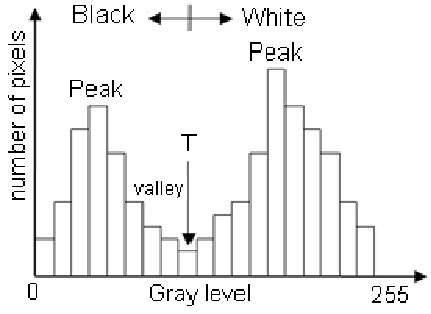
\includegraphics[width=\textwidth,height=1.7in]{obrazky-figures/Histogram-of-a-sample-gray-level-bimodal-image-T-is-the-threshold-value.pdf}}
        \caption{}\label{bimodal-hist}
    \end{subfigure}
    \hspace{0.2em}
    \begin{subfigure}[b]{.45\textwidth}
        \frame{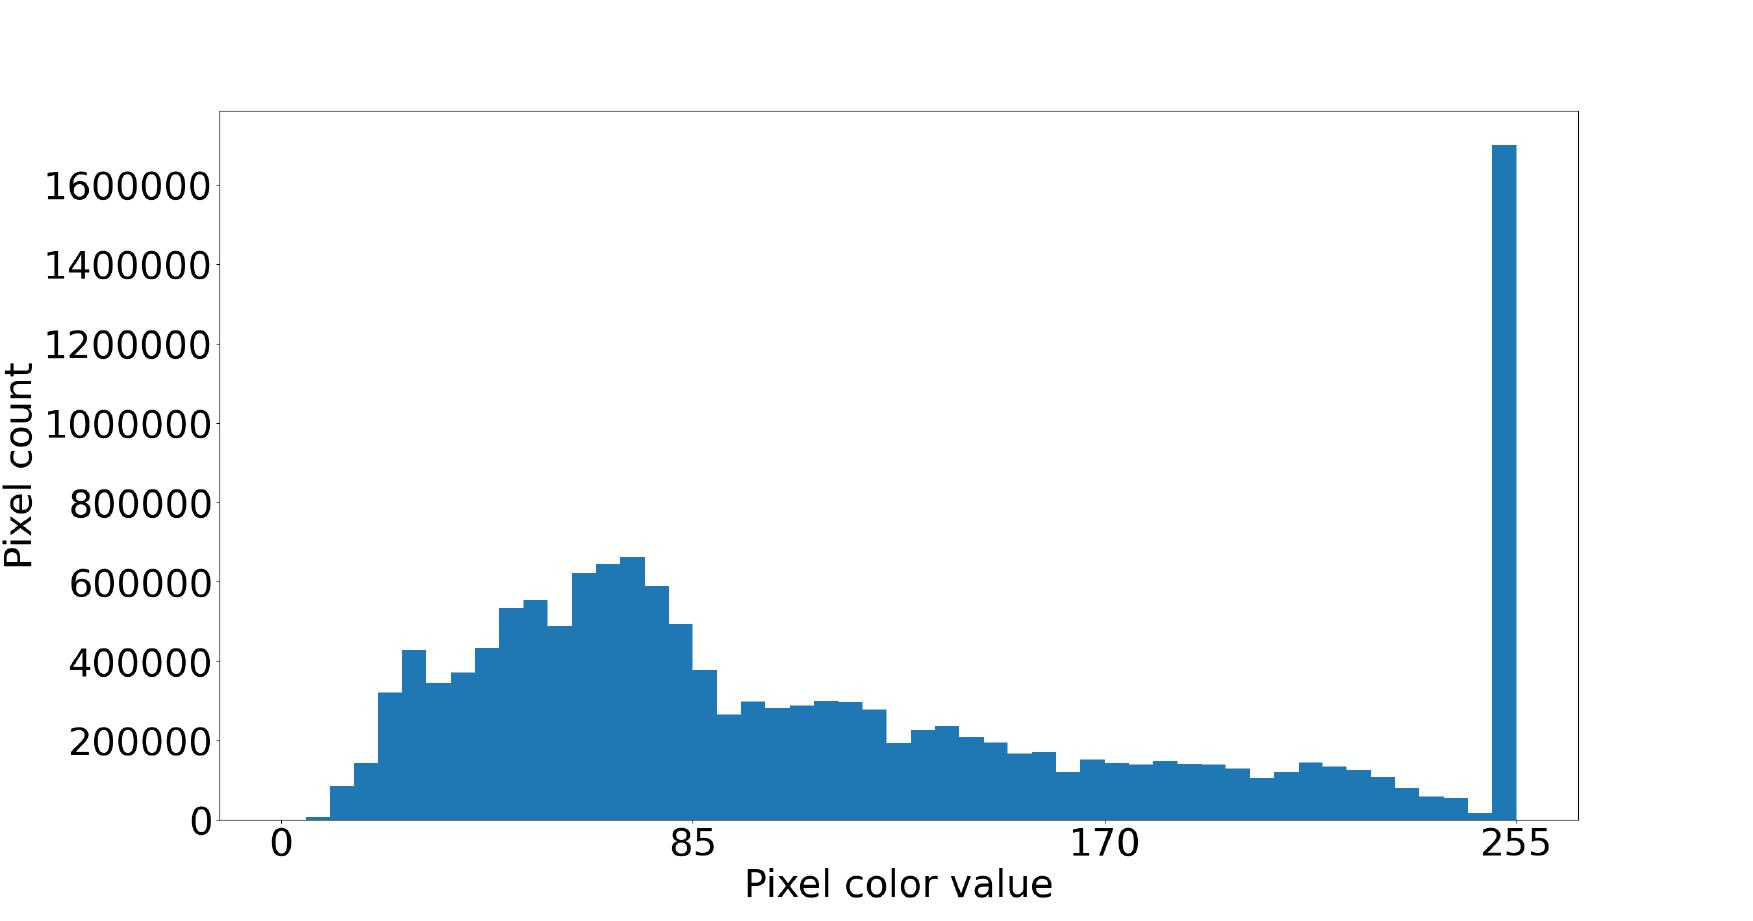
\includegraphics[width=\textwidth,height=1.7in]{obrazky-figures/otsu_hist.pdf}}
        \caption{}\label{non-bimodal-hist}
    \end{subfigure}
    \caption{\textbf{Otsu's images of histogram.} (a) Example of histogram with two peaks for bimodal image \cite{bimodal-image}. (b) Histogram of image from X-ray database.}
    \label{histograms-bimodal}
\end{figure}

\begin{figure}[ht]
    \centering
    \begin{subfigure}[b]{.3\linewidth}
        \frame{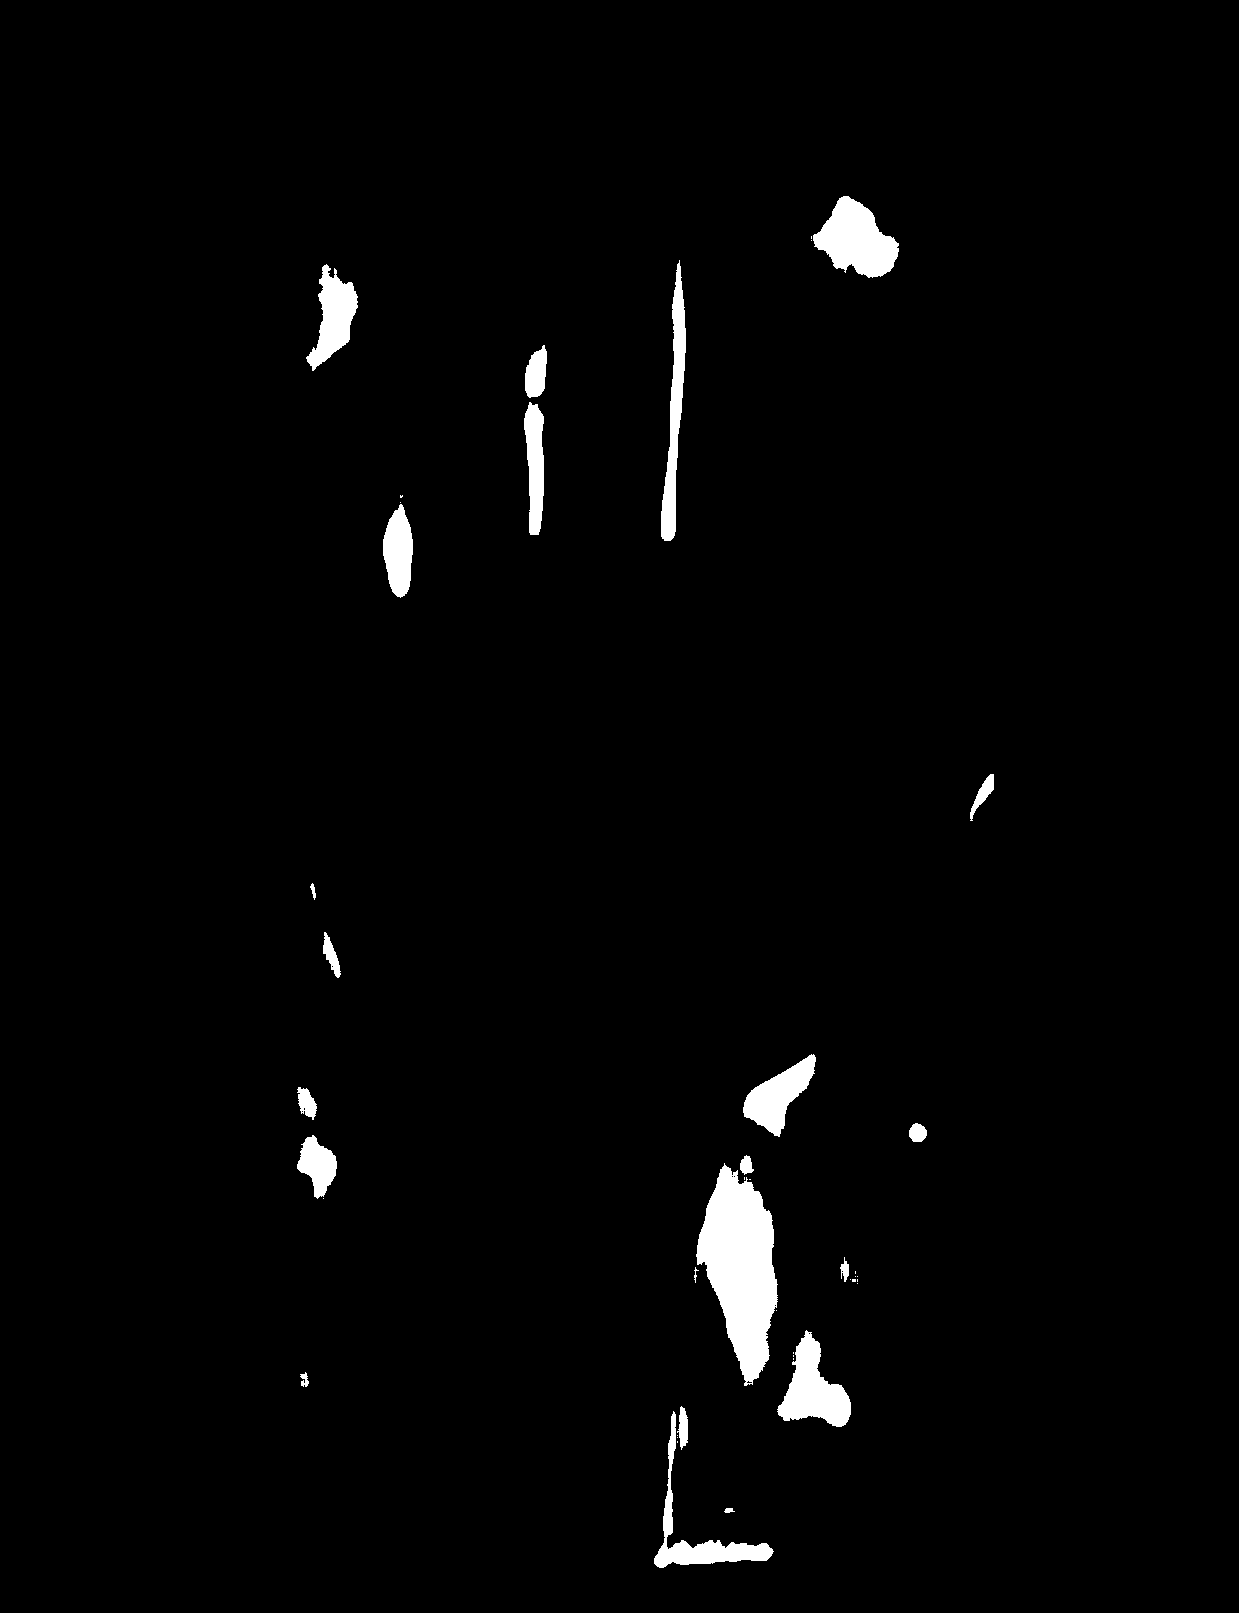
\includegraphics[width=\linewidth]{obrazky-figures/classic_thresh_normalized.pdf}}
        \caption{}\label{classic-thresh-img}
    \end{subfigure}
    \hspace{1em}
    \begin{subfigure}[b]{.3\linewidth}
        \frame{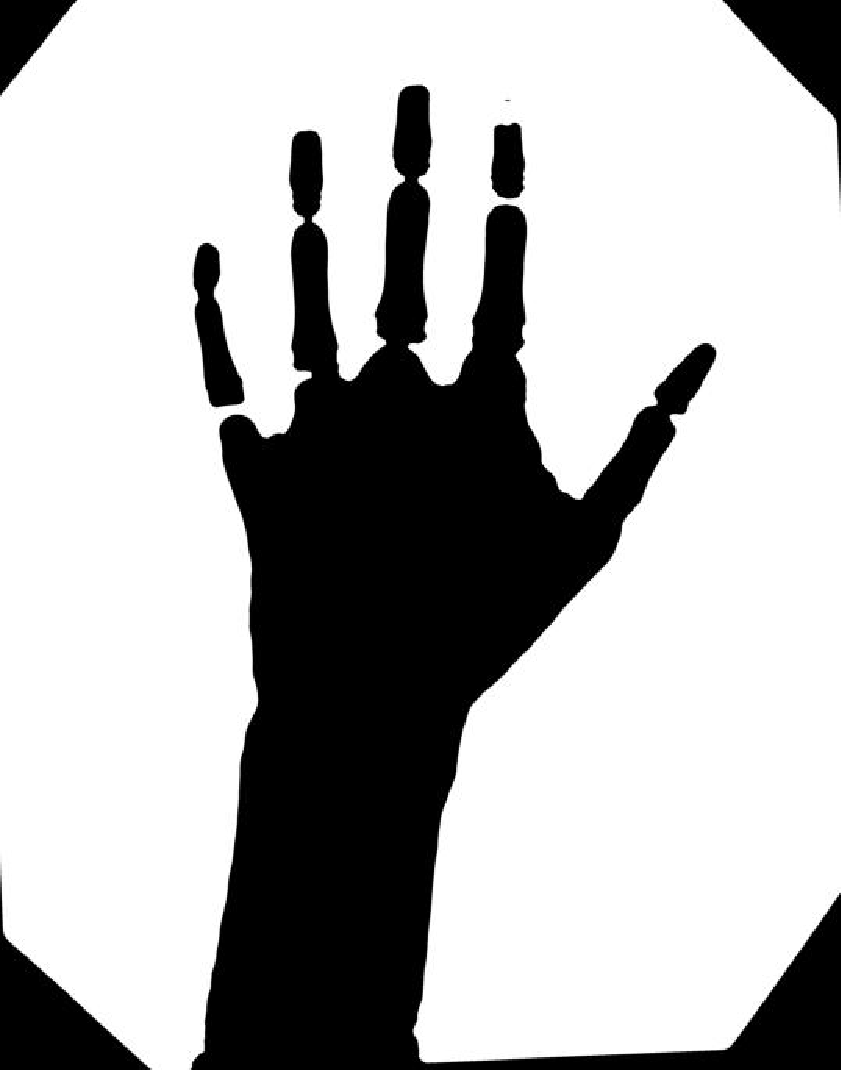
\includegraphics[width=\linewidth]{obrazky-figures/otsu.pdf}}
        \caption{}\label{otsu-thresh}
    \end{subfigure}
    \hspace{1em}
    \begin{subfigure}[b]{.3\linewidth}
        \frame{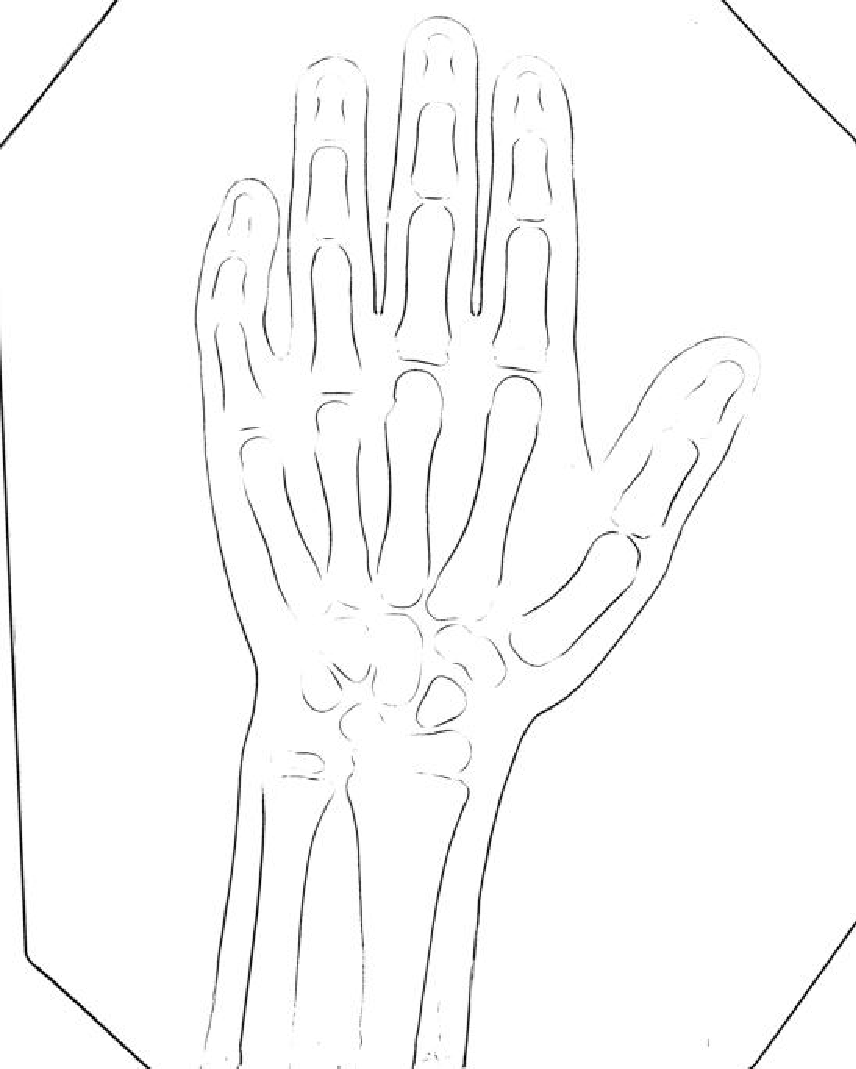
\includegraphics[width=\linewidth]{obrazky-figures/adaptive.pdf}}
        \caption{}\label{adaptive-thresh}
    \end{subfigure}
    \caption{\textbf{Thresholded pictures.} (a) Classic threshold. (b) Otsu's threshold. (c)~Adaptive threshold.}
    \label{thresholds}
\end{figure}

\subsection{Canny Edge Detection}
It is a method that is one of the most popular for edge detection, but it is certainly not suitable for every application. One of the advantages of this detector is that it is able to create edges with a width of one pixel. This edge detector is very sensitive to noise, therefore the image preprocessing is very important. The resulting output of the Canny edge detector of graphically enhanced image shows the figure \ref{canny-output} \cite{canny-edge-detector}. However, one of~the~best approaches for application of Canny edge detector is on binary image mask. This mask consists only of two pixel values which are 0 and 255. If we apply this edge detector to the image for binary mask of third metacarpal bone depicted in the image \ref{canny-mask}, then we can safely consider the output of the detector to be practically error-free, as~can be seen in~the~image \ref{canny-contour}. 

\subsubsection{Noise Reduction in Canny}
The first step of the Canny edge algorithm is a noise reduction, where a Gaussian filter is used. This filter performs convolution on the processed image to smooth the image and remove unwanted noise from the image. An example of a 5x5 convolution matrix is expressed by the equation \ref{eq:matrix} \cite{gaussian-kernel, canny-opencv}:
\begin{equation}\label{eq:matrix}
M = \frac{1}{273}
\begin{bmatrix}
    1 & 4 & 7 & 4 & 1\\
    4 & 16 & 26 & 16 & 4\\
    7 & 26 & 41 & 26 & 7\\
    4 & 16 & 26 & 16 & 4\\
    1 & 4 & 7 & 4 & 1\\
\end{bmatrix}
\end{equation}
\subsubsection{Finding Intensity Gradient of the Image}
After the smoothing effect, the image is then filtered using \textit{Sobel filter} in vertical and horizontal direction of the image matrix. Convolution matrices for obtaining a gradient by the Sobel method can be seen in the equations \ref{eq:sobel1} and \ref{eq:sobel2} \cite{sobel-matrix-opencv}:


\begin{align}
\label{eq:sobel1}
G_x &=
\begin{bmatrix}
    -1 & 0 & 1\\
    -2 & 0 & 2\\
    -1 & 0 & 1\\
\end{bmatrix}\\
\label{eq:sobel2}
G_y &=
\begin{bmatrix}
    -1 & -2 & -1\\
    0 & 0 & 0\\
    1 & 2 & 1\\
\end{bmatrix}
\end{align}

This filtration is used to obtain the first derivative in horizontal direction \(G_x\) and vertical direction \(G_y\). These derivatives can be represented as two images, from which is possible to obtain an \textit{edge gradient} using the~equation \ref{eq:gradient1} and its direction for each pixel using the~equation \ref{eq:gradient2}~\cite{canny-opencv}.

\begin{align}
\label{eq:gradient1}
    Edge\_Gradient(G) &= \sqrt{G_x^2 + G_y^2}\\
    \label{eq:gradient2}
    Angle(\theta) &= tan^{-1}  \left( \frac{G_y}{G_x} \right)
\end{align}  
\subsubsection{Non-maximum Suppression}

Main idea behind the Non\hyp{}maximum Suppression is to create thinner edges of~the~detected object. This part of~the~algorithm works by finding the pixel with the maximum value in an edge.

Pixel A in the image \ref{nms} is on the edge in vertical direction and the gradient direction is perpendicular to the edge. Pixel B and C are in gradient directions which means that pixel A is checked towards pixel B and C to check if it creates a local maximum. In case that there is created a local maximum the point is then taken to the next part of the algorithm, otherwise, it is suppressed to value of zero \cite{canny-opencv}.

\begin{figure}[!ht]
    \centering
    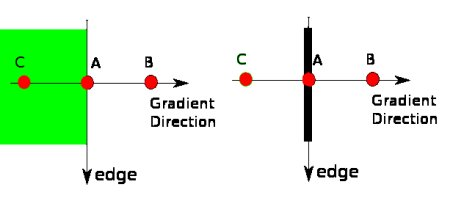
\includegraphics[width=.6\textwidth]{obrazky-figures/nms}
    \caption{\textbf{Non-maximum suppression.} Image shows algorithm detection if the pixel \textit{lies} on the edge or not \cite{canny-opencv}.}
    \label{nms}
\end{figure}

\subsubsection{Hysteresis Thresholding}
Last important part of this algorithm decides if the detected edge is the real edge or not. For~this part, two threshold values are established. First threshold value is the minimal value and the second is the maximal value. If there is any edge, which has the intensity gradient more than maximal threshold value then these potential edges are considered to~be sure edges. On the other hand, edges which has the intensity gradient value below the minimal threshold value are considered as sure non-edges and are then discarded from the detected edges. Moreover, if there are edges which has the intensity gradient between these two threshold values but at the same time are connected with the sure edges, then these edges are also considered to be the sure edges, otherwise they are considered as sure non-edges.

\begin{figure}[!ht]
    \centering
    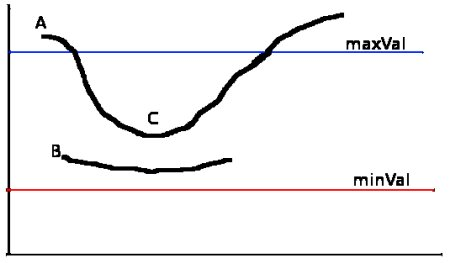
\includegraphics[width=.5\textwidth]{obrazky-figures/hysteresis.jpg}
    \caption{\textbf{Hysteresis thresholding.} Edge detection example for three different edges \cite{canny-opencv}.}
    \label{hysteresis}
\end{figure}

Image \ref{hysteresis} describes the decision making algorithm for edge detection. If there would be three different edges detected, called edge A, B and C then the thresholding is the key for making decision. As can be seen in the image, the intensity gradient is greater than the~maximal threshold value and is then considered as the sure edge. Edge B lies above the minimal threshold value but at the same time is below the maximal threshold value. In that case, if the edge is not connected with any different edge, is then considered as sure non-edge. At last, edge C is the same case as the edge B, but it is connected with the edge A which is the sure edge and thus it is also considered to~be the sure edge \cite{canny-opencv}.

\begin{figure}[!ht]
    \centering
    \begin{subfigure}[b]{.45\linewidth}
        \frame{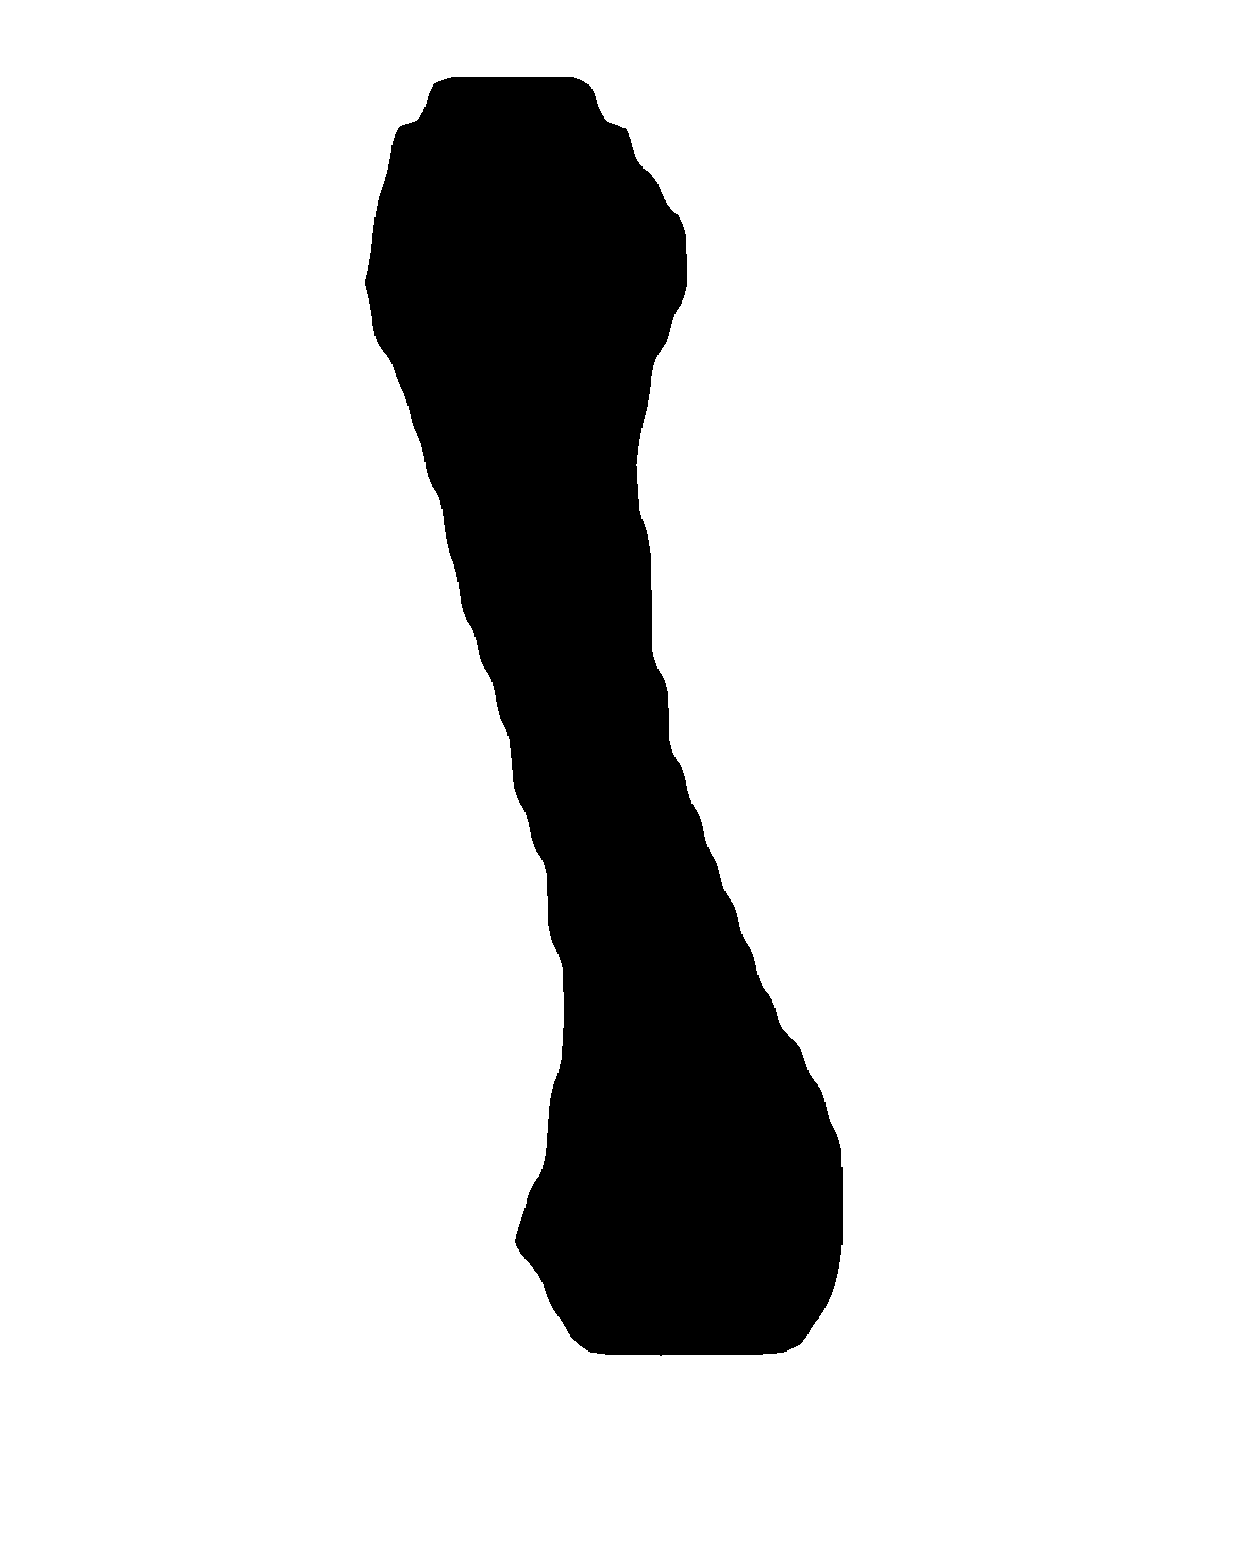
\includegraphics[width=\linewidth, height=3in]{obrazky-figures/Metacarpal_mask.pdf}}
        \caption{}\label{canny-mask}
    \end{subfigure}
    \hspace{1em}
    \begin{subfigure}[b]{.45\linewidth}
        \frame{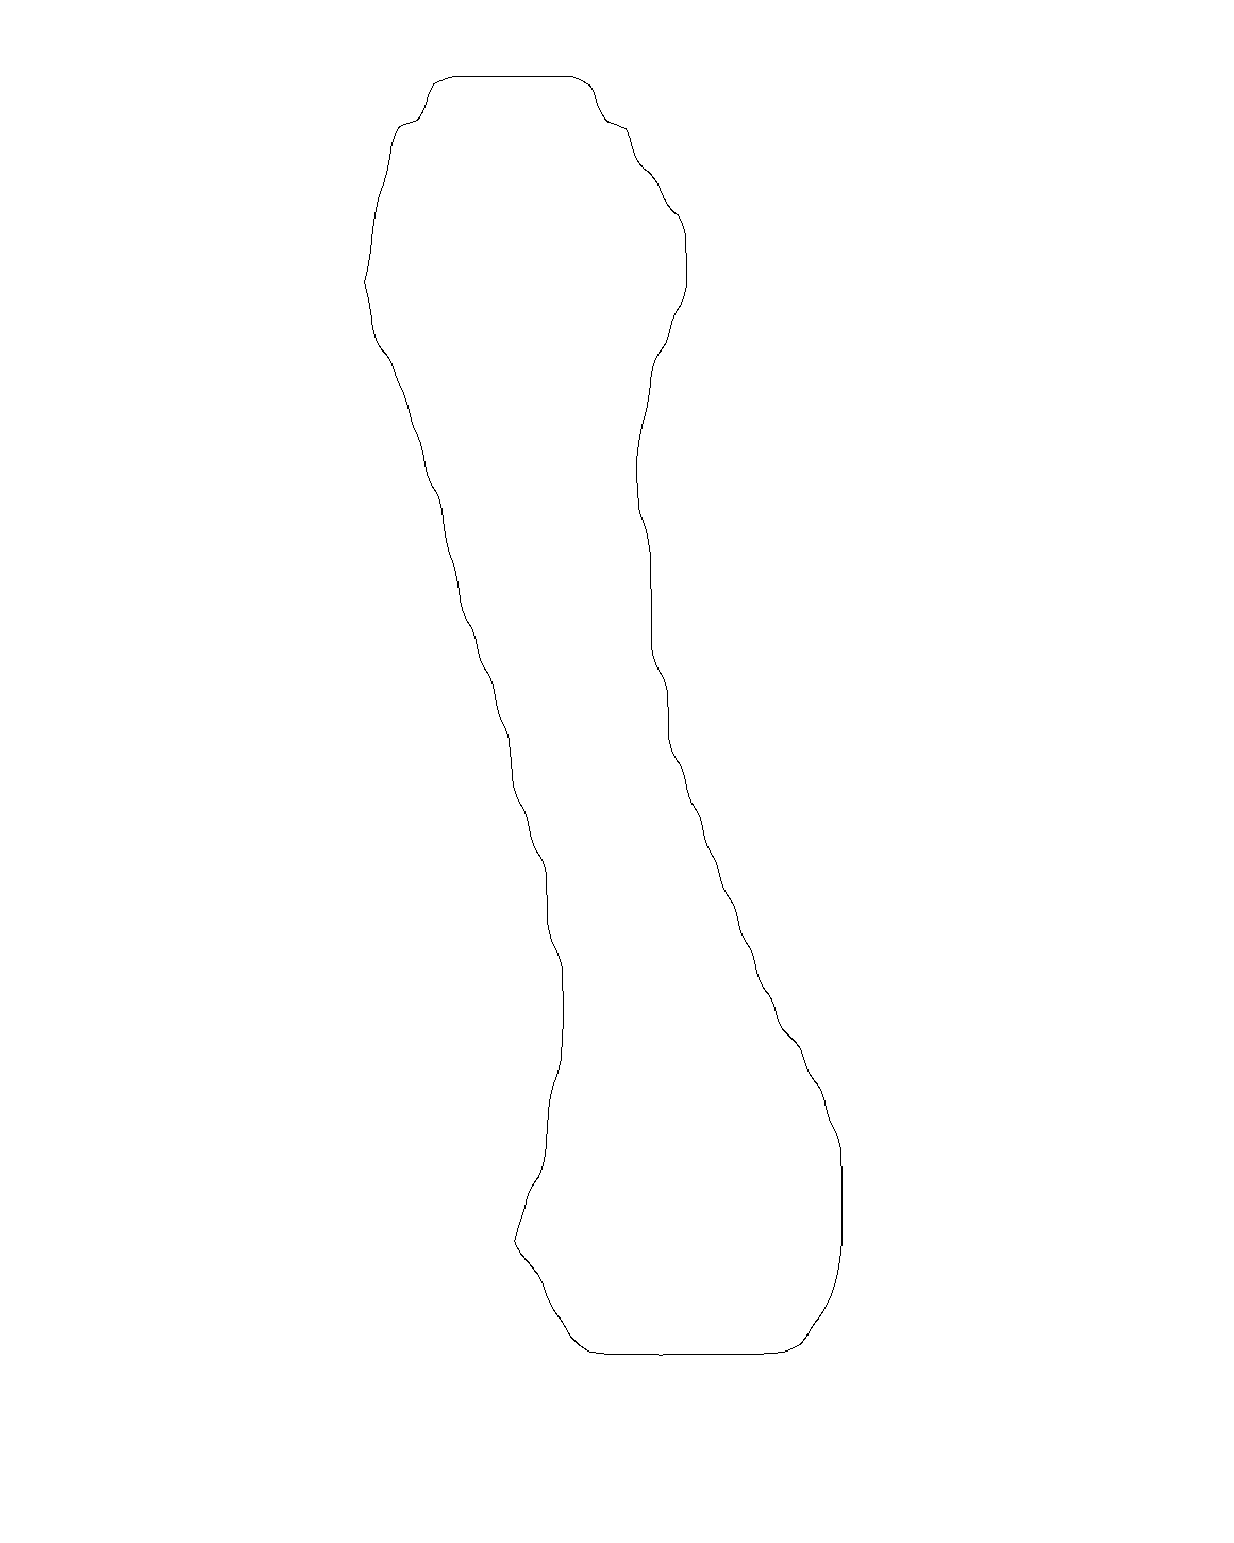
\includegraphics[width=\linewidth, height=3in]{obrazky-figures/Metacarpal_contour.pdf}}
        \caption{}\label{canny-contour}
    \end{subfigure}
    \caption{\textbf{Canny edge algorithm effect for binary image.} (a) Binary image mask. (b) One pixel wide contour obtained using Canny edge detection.}
    \label{canny-imgs}
\end{figure}

\begin{figure}[!ht]
    \centering
    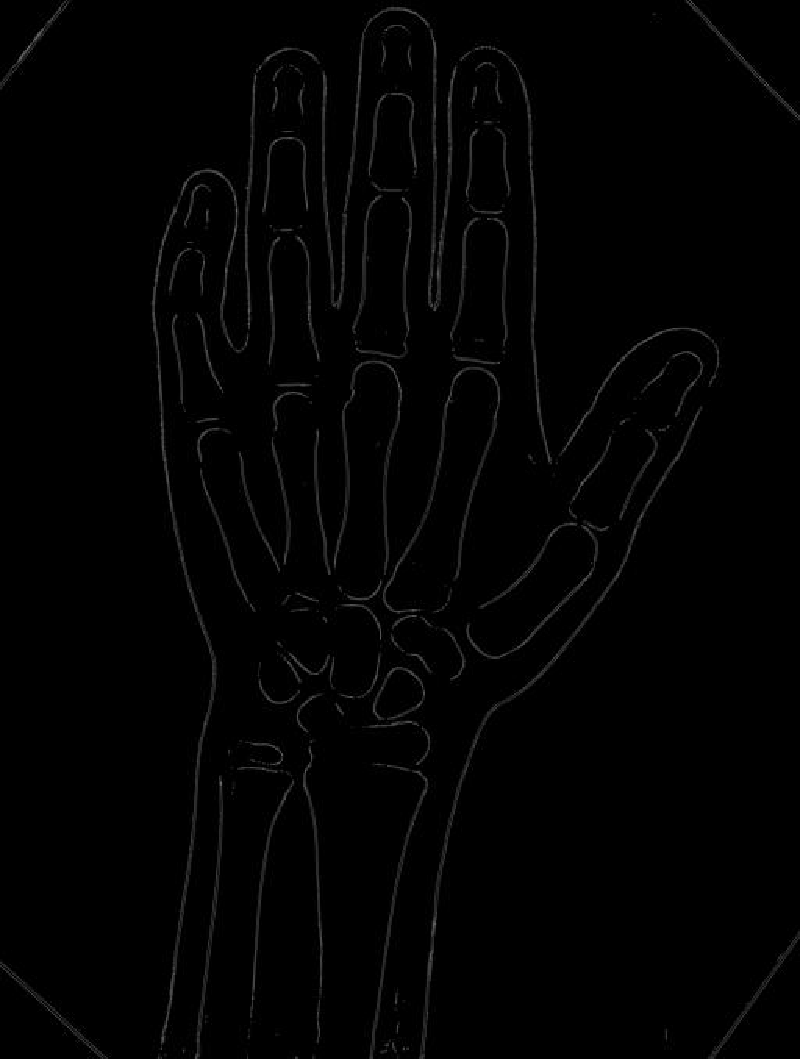
\includegraphics[width=.5\textwidth]{obrazky-figures/canny.pdf}
    \caption{\textbf{Canny edge detector output.} This image shows canny edge detector output used on noise reduced and adaptive thresholded image.}
    \label{canny-output}
\end{figure}

\section{Medical Image Segmentation}
Image segmentation in medicine has a wide range of application and is used large-scale for detailed diagnosis to uncover health problems which may not be visible to the naked eye of~a~layman. Although, at the same time, it is a demanding process, which requires choosing the most suitable method depending on the type of image, its quality and focus on the specific problem, demanding a much detailed analysis. 

The very segmentation of the image can be described as a process in which the image is being subdivided into so-called segments or subsections, all of regular or irregular shapes. This process is mostly used to find dividing lines among the objects in the image \cite{image-segmentation}.

\subsection{Semantic Segmentation}
The main goal of semantic segmentation is to classify the same or similar objects in an image under the common class \cite{semantic-semgentation, instance-segmentation}. Such classes can be anything, such as a person, a~car, a~dog, a~cat and so on. However, this object can also be something unusual, such as~the~metacarpal bones of the human hand. The image \ref{sem-seg-classes} shows a custom mask represented by matrix value of one for each classified object. One of the biggest shortcomings of semantic segmentation is that it is not able to individually label each detected object separately. In cases like this, it~would not be possible to distinguish between different dog breeds or different types of cars. This problem also occurs in the classification of the third metacarpal bone, since semantic segmentation is not able to differentiate between different types of bones. Nevertheless, this problem can be solved using another type of segmentation and that is the instance  segmentation. The~difference between these types of segmentation is shown in the images \ref{sem-difference} and \ref{inst-difference}. The~instance segmentation is described more in detail in the section \ref{instance}.

\begin{figure}[!ht]
    \centering
    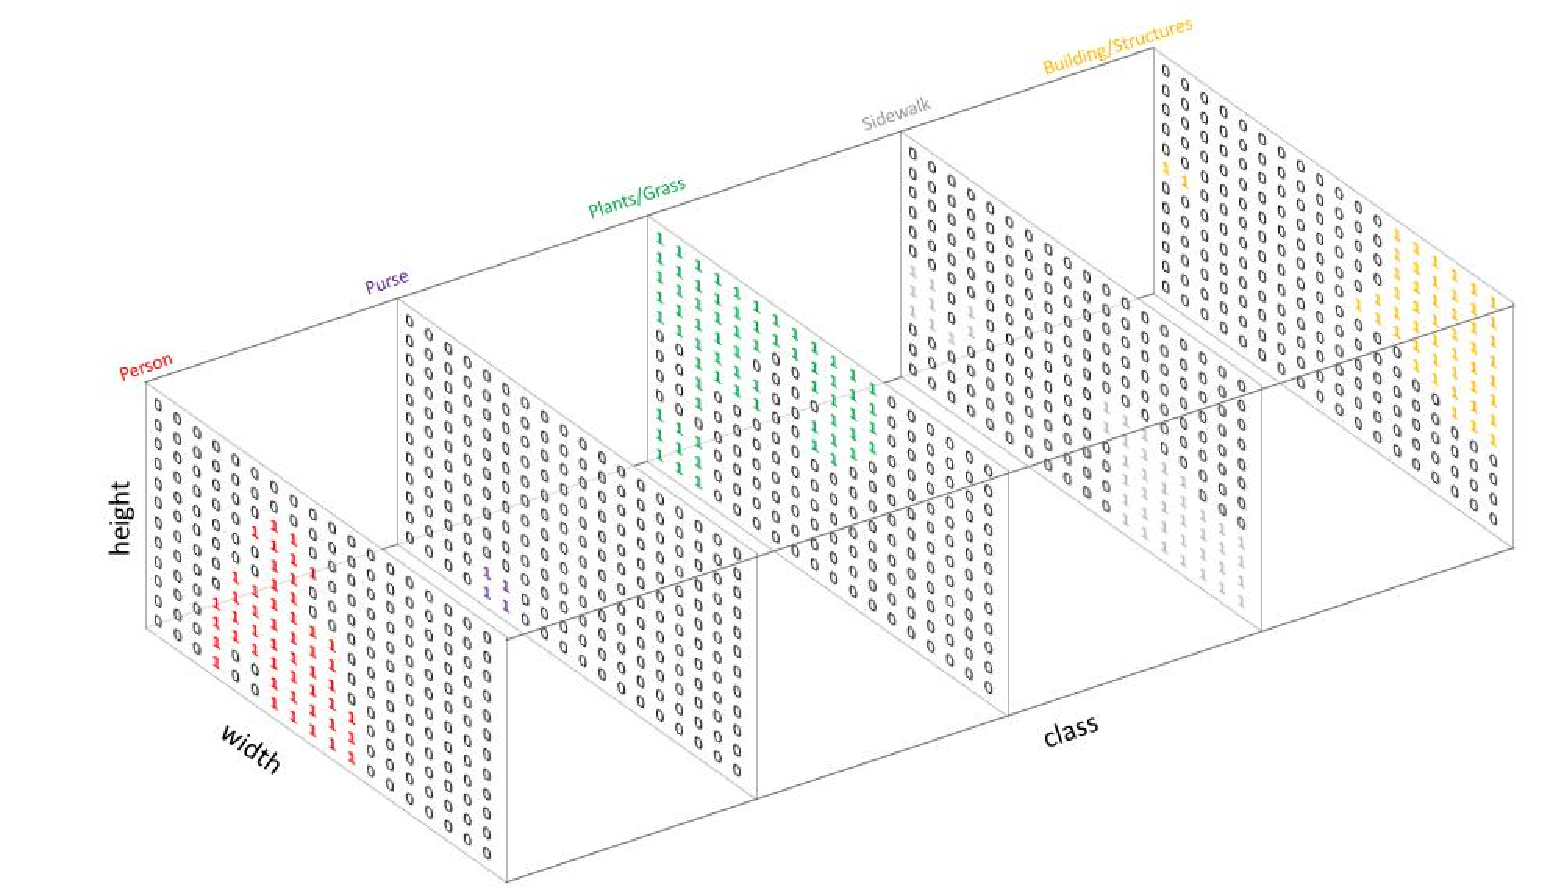
\includegraphics[width=\textwidth, height=4in]{obrazky-figures/semantic_seg_classes.pdf}
    \caption{\textbf{Semantic segmentation classification mask.} The image shows classification of individual objects in image matrix \cite{sem-seg-website}.}
    \label{sem-seg-classes}
\end{figure}

\subsection{Instance Segmentation}
The instance segmentation has one big advantage over semantic segmentation in case it~is~necessary to determine more detailed information of detected objects. This segmentation method gives different labels to detected objects in the image of the same class  \cite{instance-segmentation}. This~method, as well as semantic segmentation, is often used by CNN. In order to be able to use one of the mentioned segmentation methods, it is first necessary to train individual images using CNN and create a model from them. The training of such a model is more time consuming in the instance segmentation than, for example, in semantic segmentation. If the instance segmentation is compared to the semantic segmentation from the perspective of the detection of the third metacarpal bone, it is possible to assume that the instance segmentation will be more suitable. If it is necessary to distinguish the third metacarpus from the rest of similar-looking bone shapes, it is certainly better if this bone is detected using the method that shows the image \ref{inst-difference}. Semantic segmentation could be a more suitable method in case where it is necessary to identify whether it is, for example, bone in~the~hand or some type of soft tissue. As can be seen in the picture \ref{detectron-instance-seg}, the result of one of the~algorithms, which will also be described in the section \ref{cnn-design}, is relatively precisely drawn bone mask and therefore it appears as one of the appropriate approaches to segmentation of the third metacarpus.

\label{instance}
\begin{figure}[!ht]
    \centering
    \begin{subfigure}[b]{.4\textwidth}
    \centering
        \frame{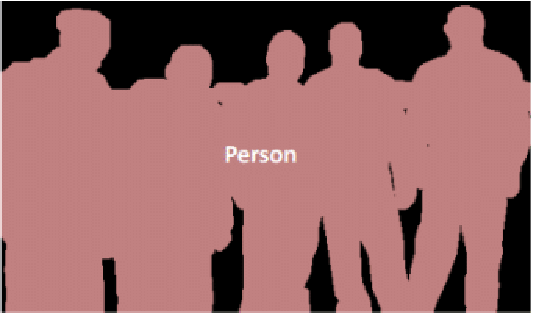
\includegraphics[width=.85\textwidth]{obrazky-figures/semantic_example.pdf}}
        \caption{}\label{sem-difference}
    \end{subfigure}
    \begin{subfigure}[b]{.4\textwidth}
    \centering
        \frame{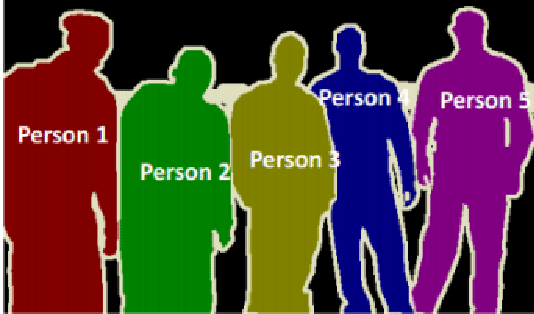
\includegraphics[width=.85\textwidth]{obrazky-figures/instance_example.pdf}}
        \caption{}\label{inst-difference}
    \end{subfigure}
    
    \begin{subfigure}[b]{.4\textwidth}
    \centering
        \frame{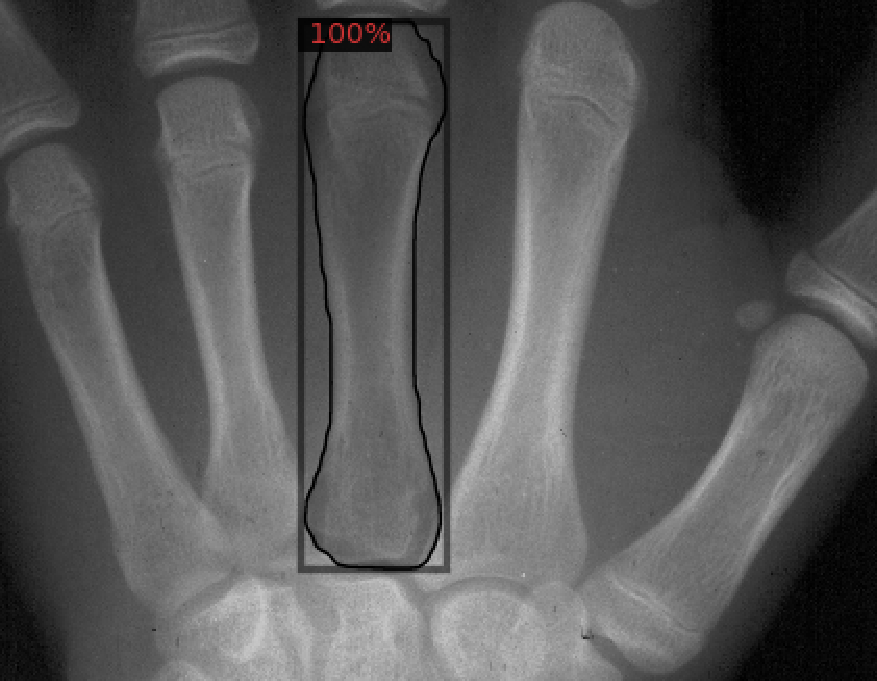
\includegraphics[width=.85\textwidth]{obrazky-figures/bez_stvorca.pdf}}
        \caption{}\label{detectron-instance-seg}
    \end{subfigure}
    \caption{\textbf{Semantic and instance segmentation comparison.} (a) Semantic segmentation example \cite{semantic-vs-instance-seg}. (b) Instance segmentation example \cite{semantic-vs-instance-seg}. (c) Result of instance segmentation on X-ray database image.}
    \label{sem-seg-comparision}
\end{figure}

\subsection{Watershed Segmentation}
\label{watershed}
Watershed algorithm, whose essence is derived from natural and basic behavior of natural elements is very important and frequently used in medical image segmentation \cite{watershed-segm}. The~image can be portrayed as topographic surface, which is made of so-called ridges and valleys. If~we~consider an image in 3D-form, in which the light areas are ridges~and~dark areas are valleys, we can define a concept of catchment basins. Then, the algorithm segments thus created catchment basins. The problem occurs if the image is too noisy and~as~a~result, oversegmentation appears. This can cause a formation of large amount of regions or so-called segmented areas \cite{watershed, many-approaches}. Therefore, it is very important to create adequate image enhancement. Image \ref{watershed-img} shows watershed segmented image with proper image enhancement.

\begin{figure}[!ht]
    \centering
    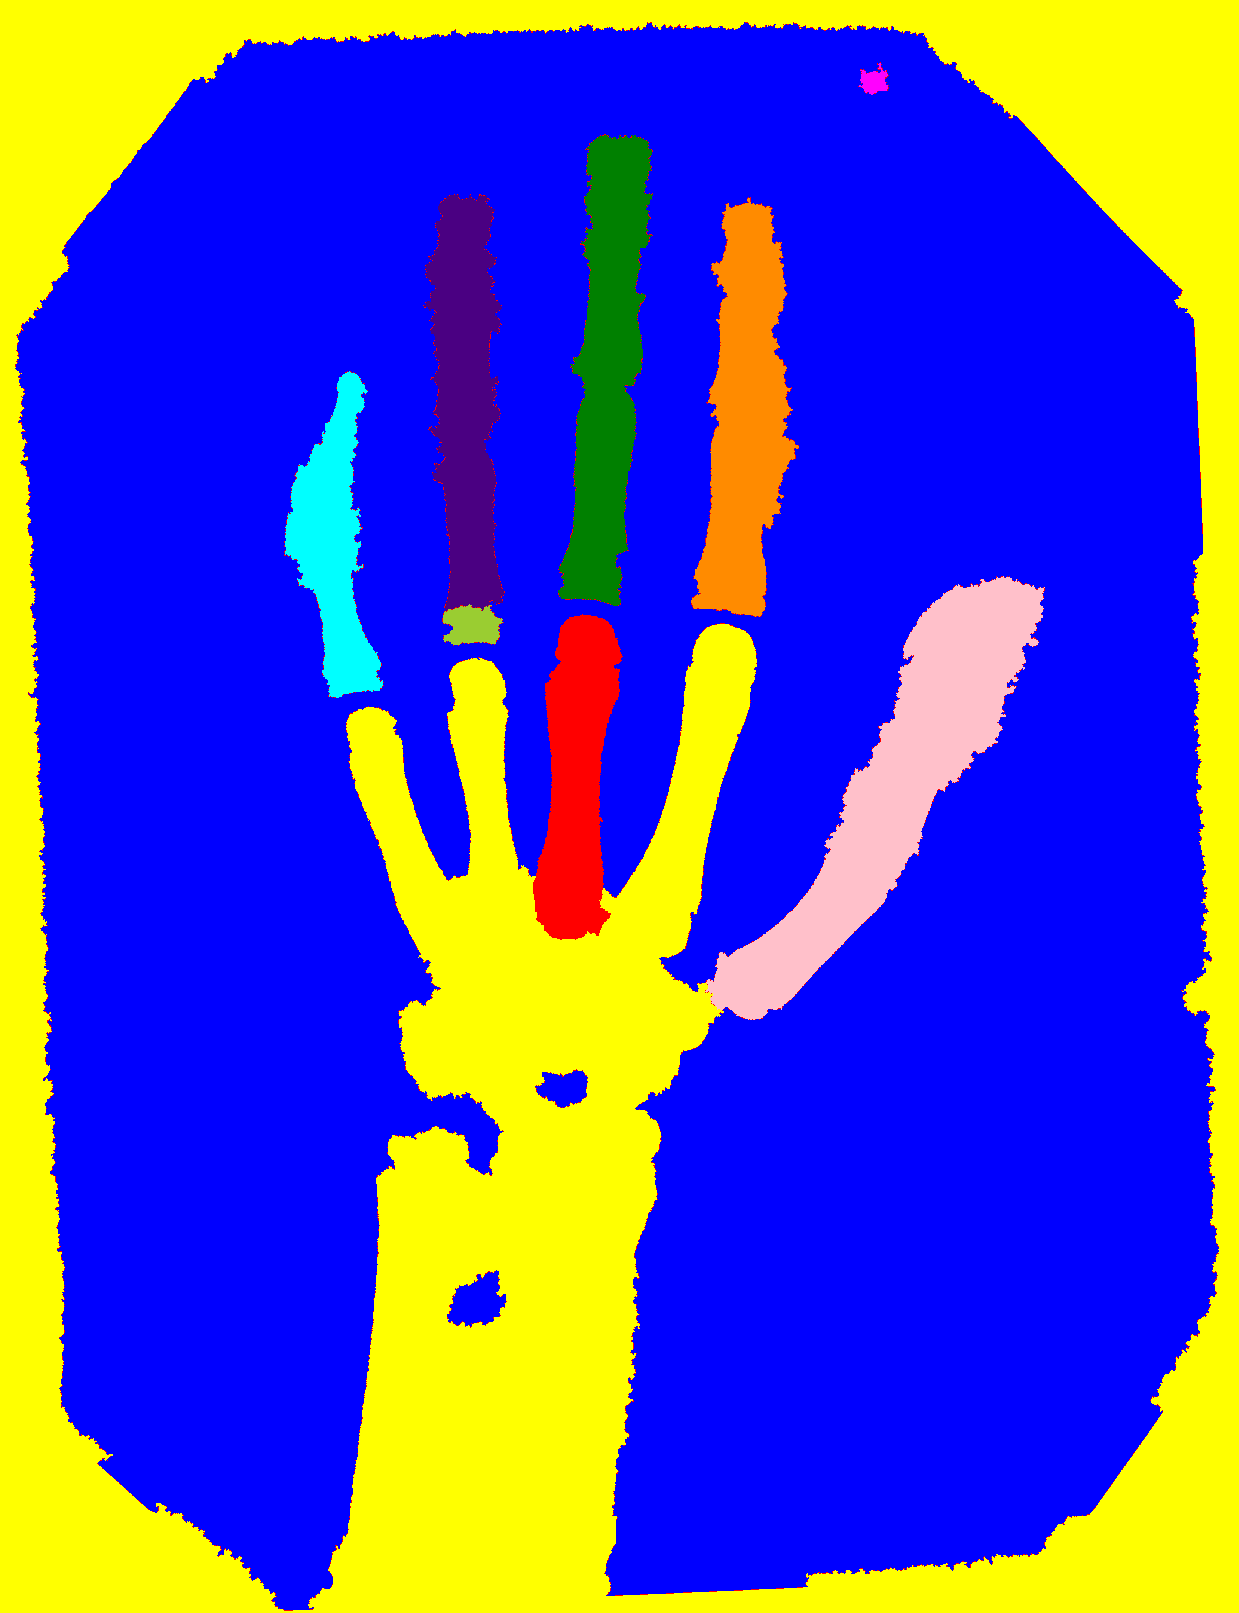
\includegraphics[width=.35\textwidth]{obrazky-figures/watershed2.pdf}
     \caption{\textbf{Watershed image segmentation output.} Image shows the result of watershed segmentation on one of the X-ray database image. Many inaccuracies can be observed in this method output.}
    \label{watershed-img}
\end{figure}

\section{Supervised Learning}
Quality methods for pattern recognition often utilize training dataset that contain many well annotated images. Training dataset has inputs and correct outputs. These two states allow the model to learn over time. During the learning process the algorithm measures its accuracy through the so-called loss function\footnote{Loss function evaluates how good is the model created on training dataset. In case the predictions are not well, the loss function will output the higher number, otherwise the output of loss function will be lower number \cite{loss-function}.}, adjusting until the output of the loss function is minimal number. In this thesis, there is used supervised learning based on~manual image annotations of the third metacarpal bone using neural networks algorithm \cite{ibm-supervised-learning, supervised-learning-paper}. Supervised learning uses training data on the basis of which a final test model for future inference is then created. In case of X-ray images, inference will be performed on the database of~images from the anthropological institute for segmentation and contour detection of the~third metacarpus.

\begin{figure}[!ht]
    \centering
    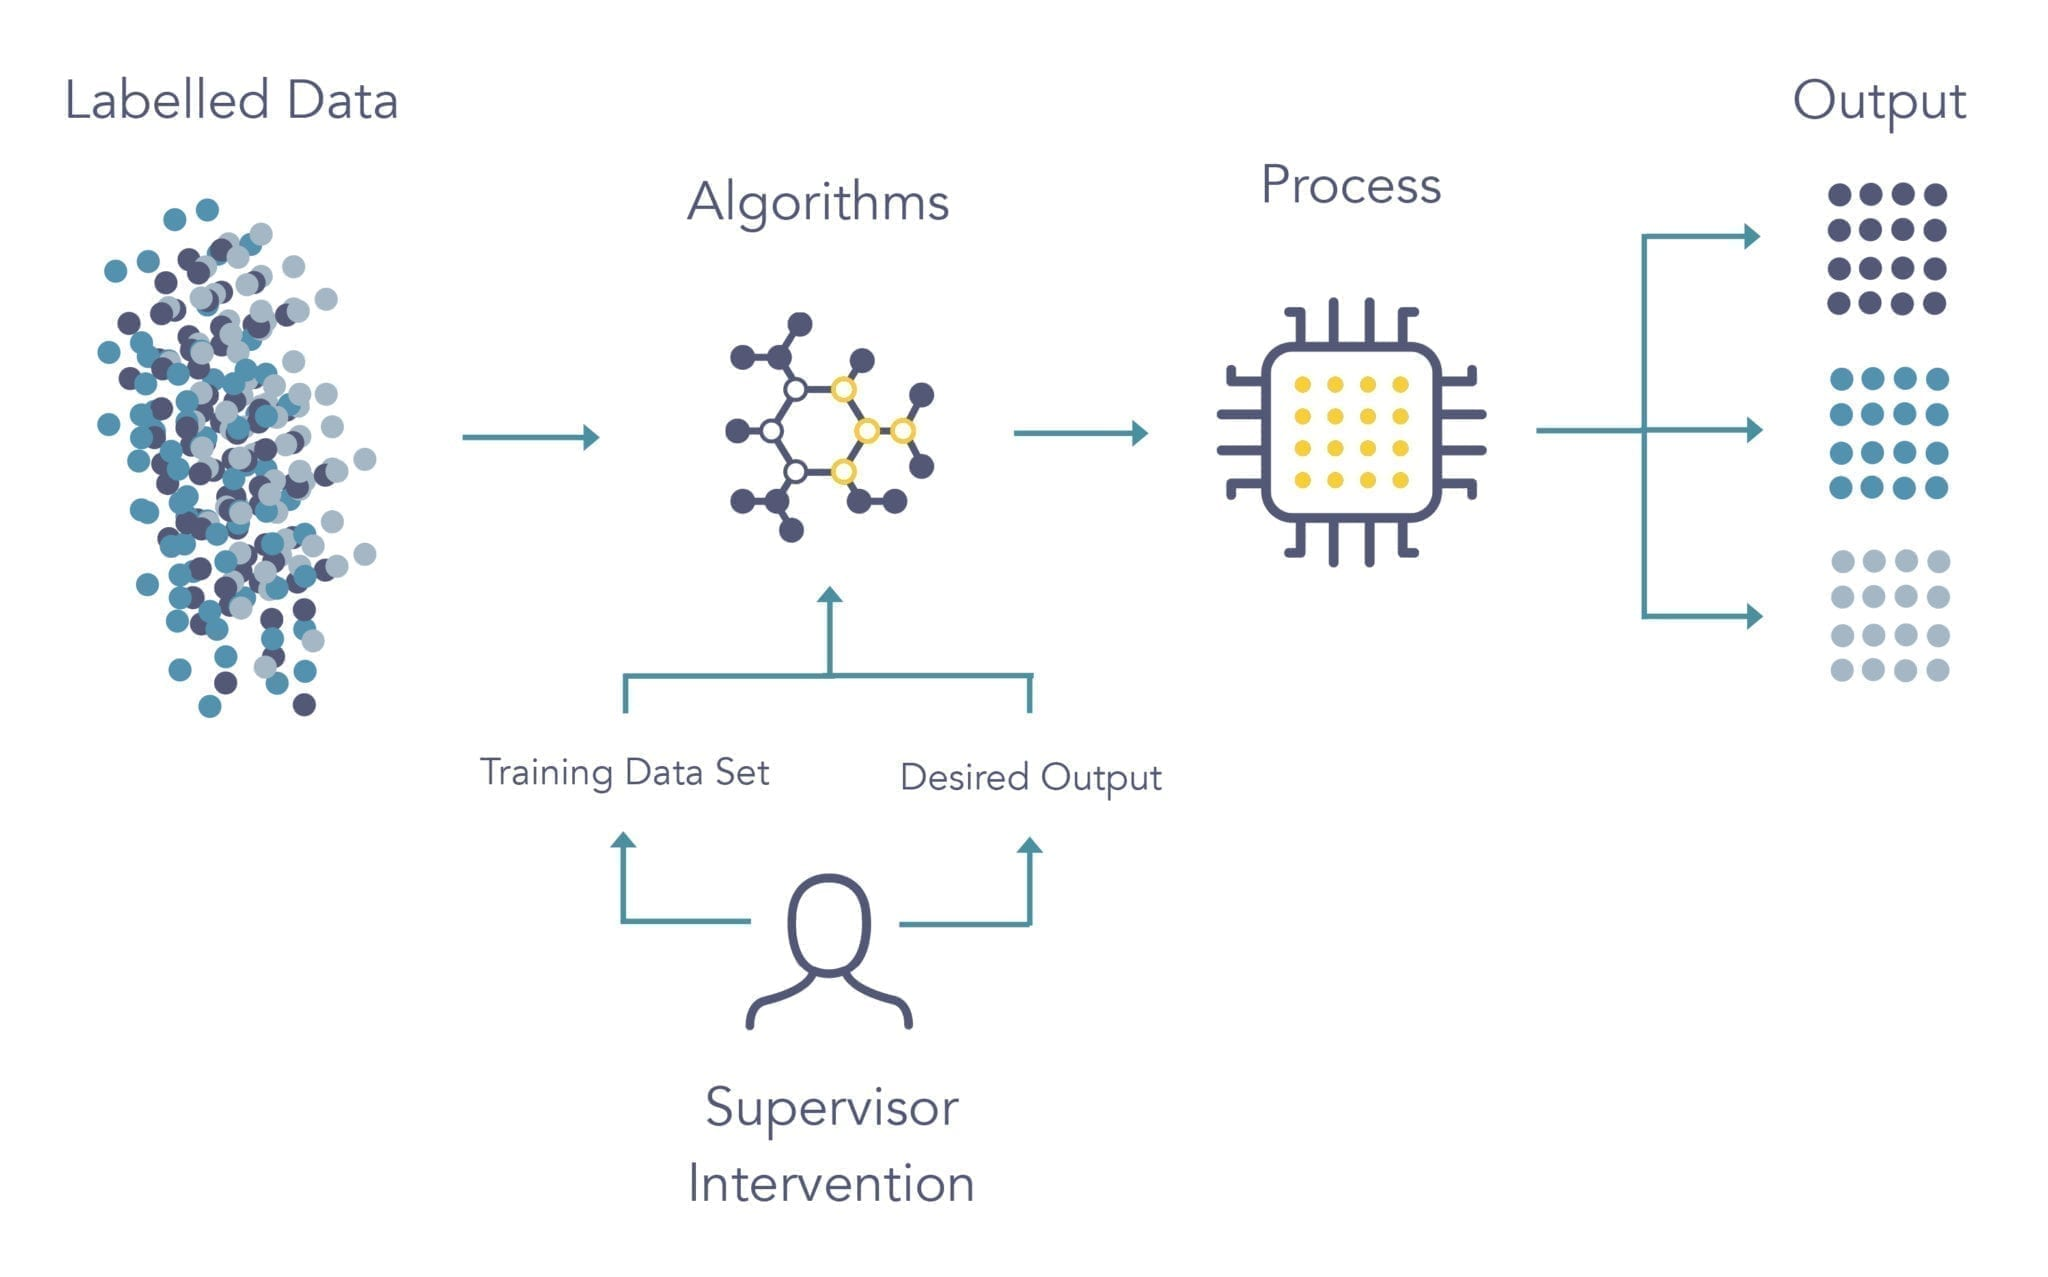
\includegraphics[width=.75\textwidth]{obrazky-figures/machine-learning-infographics-2-scaled.jpg}
     \caption{\textbf{Supervised learning.} Image shows basic idea of supervised learning \cite{supervised-learning}.}
    \label{supervised-img}
\end{figure}

\subsection{Mask Region-based Convolution Neural Network (Mask R-CNN)}
\label{mask-rcnn-framework}
According to \cite{mask-rcnn}, Mask R-CNN is an extension of Fast R-CNN, which consists of two parts. The first part is the region proposal network (RPN), which features bounding rectangles for mandatory objects. Next part extracts features using RoIPool\footnote{According to \cite{Pooling} Region of Interest Pooling creates the fixed-size feature maps from non-uniform inputs using the operation of max-pooling on the inputs.} from each candidate box and performs classification and bounding-box regression\footnote{Bounding-box regression is technique to refine or predict bounding boxes in object detection \cite{bbox-regression}.}.

%TODO
\section{Image Processing Tools}
Nowadays, to achieve algorithmic results in image processing, it is possible to use one of~many available tools or libraries. They can be applied in gradual decomposition of~problems in the image pre-processing and its analysis. Working with the digital image, of~course, is not easy and requires
many mathematical operations, which are often computationally demanding and algorithmically complicated. In such case, it is convenient to use one of~already available tools to work with computer vision.

\subsection{OpenCV}
One of the most famous libraries available to public is OpenCV. The library has a wide range of algorithms, which are optimized at speed and provide high rate of abstraction of~the~algorithm functionality, and therefore bring simplicity and effectivity together into work itself. This thesis uses algorithms for image processing, segmentation and edge detection.

%TODO
\subsection{Detectron2}
In addition to libraries and tools that use traditional methods for working with images, such~as OpenCV, there are also libraries that can be used, for example, for image processing using neural networks. Detectron2 is a library that offers several ways to perform pattern recognition, such as semantic or instance segmentation. The~library~contains~several~ImageNet\footnote{\url{https://imagenet.stanford.edu/}} pre-trained models that can be used to create a custom model to solve~a~specific problem. If the framework from the section \ref{mask-rcnn-framework} is used, it is possible to use baselines based on FPN\footnote{\url{https://arxiv.org/abs/1612.03144}} (Feature Pyramid Network) in combination with ResNet\footnote{\url{https://arxiv.org/abs/1512.03385}} (Residual Neural Network) backbone for mask and box prediction. These models provide the created architecture for CNN, thanks to which it is not necessary to create your own architecture for neural networks, which greatly facilitates the work itself and the creation of a reliable model. When working with the library itself, the use of GPU acceleration is very effective, however, if the computing device does not have a quality graphics card, it is possible to use only the basic computing unit (CPU) for calculations. Detectron2 uses Python syntax and contains a custom abstraction with a number of functions that can be used to create~a~custom image segmentation model, for example using the instance segmentation method, and perform inferences on test data at the same time. The output after inference is an input image with a predicted mask, such as in the image \ref{detectron-instance-seg} \cite{detectron2}.
%%%%%%%%%%%%%%%%%%%%%%%%%%%%%%%%%%%%%%%%%%%%%%%%%%%%%%%%%%%%%%%%%%%%%%%%%%%%%%%%%%%%%%%%%%%%%%%%%%%%%%%%%%%%
\chapter{Designed Solution and Implementation}
\label{chapter3}
At first, this chapter describes an algorithms based on empirical discoveries of the tested methods for image noise reduction, edge detection and usage of traditional segmentation methods for pattern recognition. Created flowchart for this solution can be seen in image~\ref{flowchart1}. This chapter also describes designed solution for desired algorithm using CNN which seems to be more usable than the classic segmentation methods. Furthermore, this chapter describes the advanced algorithm extension which is mainly focused on measurement of~the~bone in more detail than just the basic algorithm. At last, this chapter explains the~basic usage of the algorithm including tools which were used for development and the~simple directory tree structure of the program.

\begin{figure}[!ht]
    \centering
    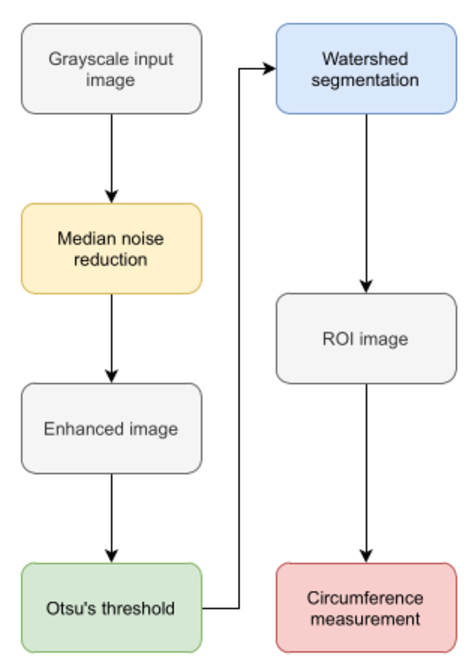
\includegraphics[width=.4\textwidth]{obrazky-figures/unsuccessful.pdf}
    \caption{\textbf{Flowchart.} Image depicts flowchart for pattern recognition using traditional methods.}
    \label{flowchart1}
\end{figure}

\section{Analysis of Medical Images Issues}
For a correct design, it is essential to determine and analyze any possible issues that might appear in X-ray image processing beforehand. It is important to realize that despite the~resemblance of the images, every individual image is different and displays bones of the hand of people of different age and sex. One of the primary problems which requires attention is so called overlap of the bones, which can be caused for instance by the wrong position of~the~hand on the scanning device as well as by the age of the concerned patient.

Another issue might be a defective result of the illumination of the bone itself. Any errors may be caused by the position of the hand towards the device responsible for sending out X-rays or by the contents of inorganic substances in the bones, as they result in higher density. Third metacarpal bones are mostly light in their middle part which is the body of the bone. Contrariwise, in the area of the head and the base of the bones they are darker, which shows a negative effect on the edge detection, because it is dependent on~clear transition between light and dark shade of grey \cite{metacarpal-structure}.

Last of the analyzed problems is the very imperfection of the created 2D X-ray images, which causes complications for the measurement phase of the width of the third metacarpal bone. To securely measure the width of the bone in its narrowest area, there has been a~mathematical model designed using analytical approach.

\section{Median Noise Reduction}
This smoothing filter was used based on testing of multiple smoothing filters, among which the median filter achieved the best results for X-ray images. It is an effective way which is not computationally difficult and at the same time the edges are preserved for further use.

\subsection{Proposed Otsu's Threshold}
Among all the threshold methods that were presented in the section \ref{classic-thresh}, the most suitable way was to use Otsu's threshold, thanks to which it was possible to follow well on~the~following methods in image processing, which very well separates the~foreground from the background of the image. By thresholding, an approximated area is obtained where the~hand is on the X-ray image, which is sufficient information for watershed segmentation.

\section{Application of Watershed Segmentation}
The principle of algorithm watershed was described in part \ref{watershed}. This way of segmentation is often used while segmenting medical image and it is very sensitive to noise which can lead to oversegmentation \cite{many-approaches, third-metacarpal-approach}. However, if the image is pre-processed well, the algorithm is able to deal with the problem of overlapping of the bones quite easily and effectively. Overlapping occurs in most of the cases of the images in dataset. The algorithm was relatively effective in separating the individual regions that are in the image, but the results of segmentation are very inaccurate and practically unusable for further use. As can be seen in the picture \ref{watershed-img} the third metacarpus was separated from the remaining bones, which was proved mainly due to the good position of the bone, which did not interfere too much with the secondary bones and could also contribute to appropriate illumination of the picture. However, this approach worked only for a few images from the entire database, which causes problems for the robustness of the algorithm, which must work for the statistical majority of images, so it is possible to assess that segmentation using traditional methods is unusable to solve a problem that would be sufficient for anthropological department.

\section{Canny Edge Detector Applied for Watershed}
After using the watershed segmentation method, the edges were detected using Canny edge detector. This method is one of the essential steps after segmentation of the image. However, in this case, the results of watershed segmentation are not as good as necessary for a high quality edge detection. The results of application for Canny edge method can be seen in image \ref{water-canny}. This edge detection was applied for the segmented hand from the~picture~\ref{watershed-img}.

\begin{figure}[!ht]
    \centering
    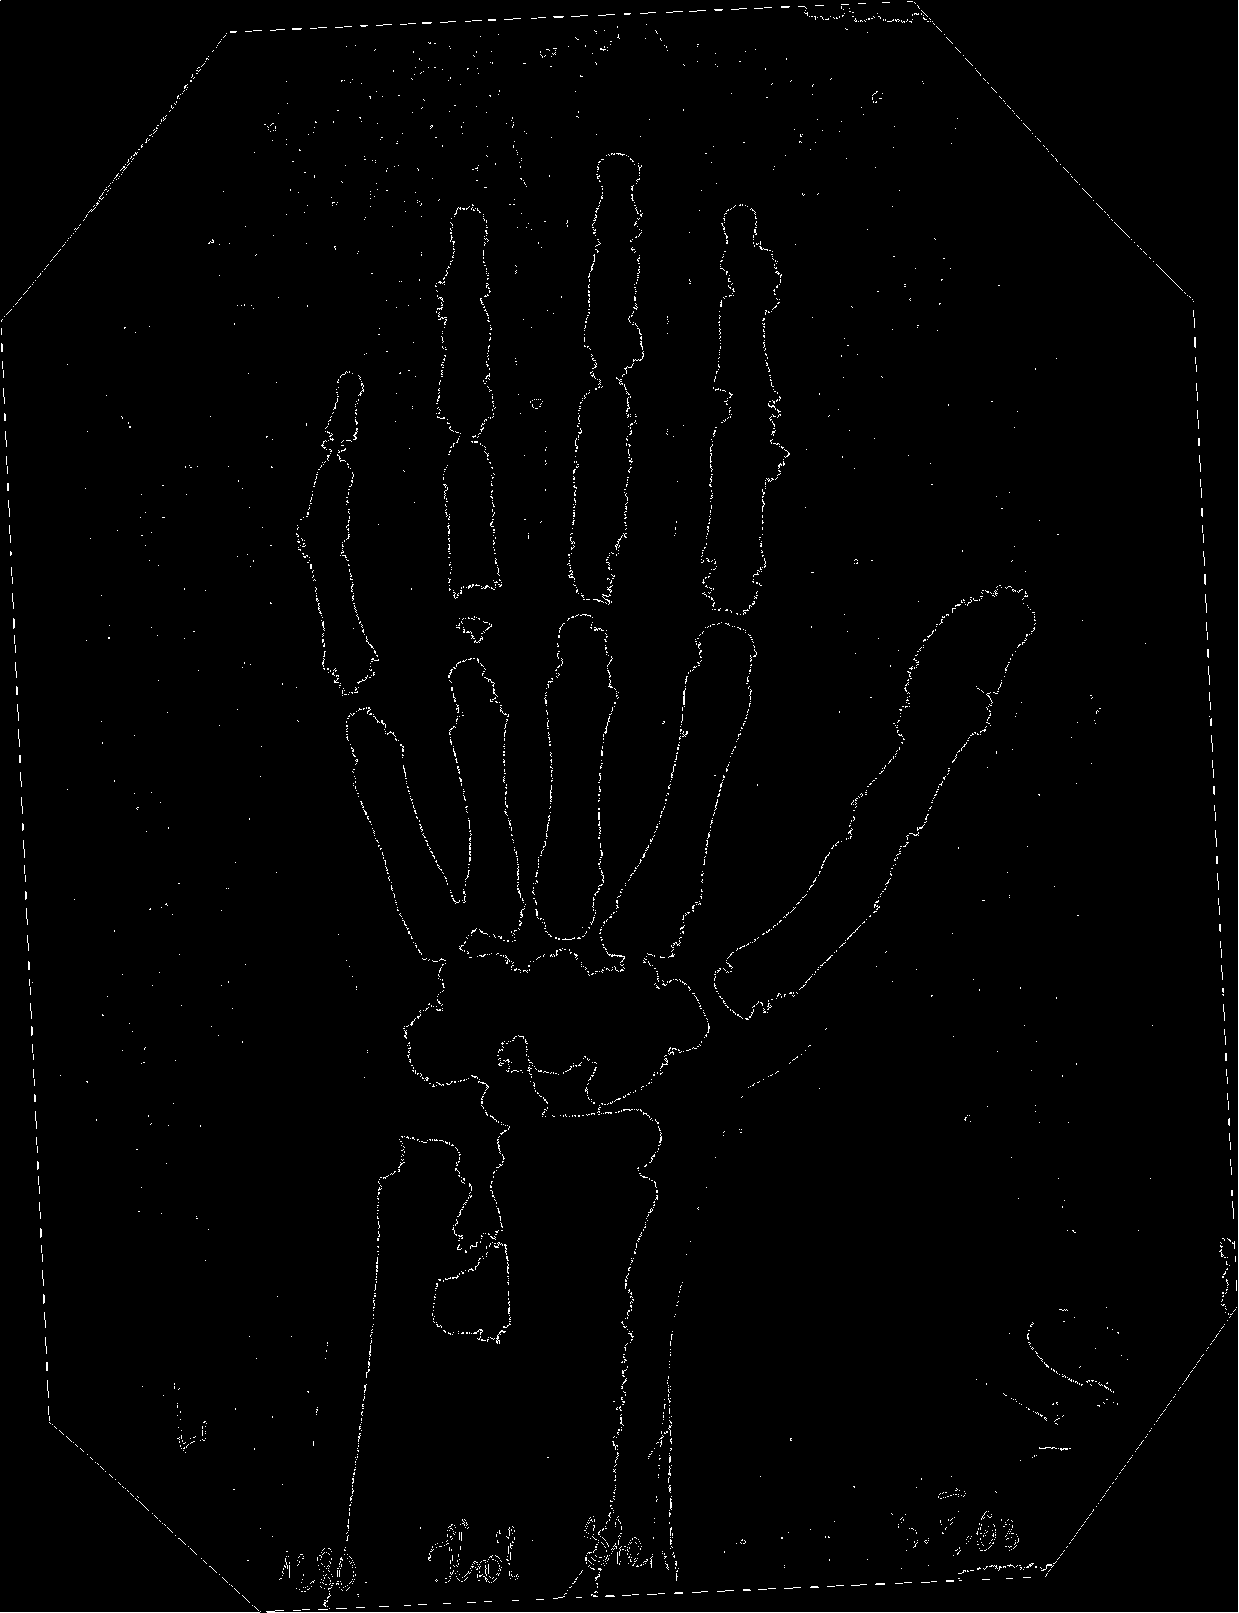
\includegraphics[width=.5\textwidth]{obrazky-figures/water_canny.pdf}
    \caption{\textbf{Canny edge application.} Image shows the application of the edge detector after watershed segmentation.}
    \label{water-canny}
\end{figure}


\section{Evaluation of Tested Methods Issues}
To create a correct algorithm design, it was necessary to test algorithms for preprocessing and segmentation of the image and analyze the achieved results. Afterwards, it was possible to draw a conclusion regarding which of the algorithms was the most suitable one. This~particular situation leads us to the conclusion that it is not possible to use only a~simple watershed segmentation, as it is not competent to sufficiently deal with the overlap of~the~bones. It is necessary to use a more complex segmentation algorithm to detect the~edges more clearly.

%%%%%%%%%%%%%%%%%%%%%%%%%%%%%%%%%%%%%%%%%%%%%%%%%%%%%%%%%%%%%%%%%%%%%%%%%%%%%%%%%%%%%%%%%%%%%%%%%%%%%%%%%%%%
\section{Design for Pattern Recognition with CNN}
\label{cnn-design}
Since the use of traditional methods for pattern recognition has not proved to be a reliable method, it is essential to choose a method using convolutional neural networks. By~creating a model using the Detectron2 library, the algorithm will predict the mask of the~third metacarpal bone. This chapter also interprets actual process of contour detection and calculation of the width of the third metacarpal bone in the area where the bone reaches its most narrow diameter. The algorithm is designed to function properly in an~available dataset of~X-ray images and to provide uniform results for the statistical majority of~the~processed images. One of CNN’s strong points is no need to use pre-processing methods, such~as~noise reduction or normalization. Despite the fact that the segmentation of traditional methods failed in the approach from the beginning of the chapter \ref{chapter3}, even these methods won't be avoided completely. After obtaining the mask, which is the most important task in~CNN usage, it is necessary to display the bone as a binary image, which is very effectively aided by~the~classic separation of foreground from background, which in this case will not be~performed by any of the OpenCV library function but a specially created function. Extraction of~a~bone contour in the width of one pixel can be performed using the Canny edge detection method, which works error-free for a binary image with removed artifacts. Individual steps of the designed algorithms are displayed in the proposed flowchart~\ref{flowchart2}.

\subsection{Using Mask R-CNN by Detectron2}
As mentioned in previous sections, the proposed algorithm for bone mask segmentation uses a specially created convolutional neural network Mask R-CNN, which is built into the~library Detectron2, and therefore will be the main focus and starting point in this chapter. 

\subsection{Custom Model Creation}
To predict the mask, it is necessary to train the model, which will detect the third metacarpal bone from X-rays. The Detectron2 library is used to train the model, which enables the~creation of a custom model. In order to create that, it is necessary to~annotate a certain part of~X-ray images, specifically the third metacarpus, thanks to~which it~is possible to determine the so-called ground truth image\footnote{Ground truth image in conjunction with machine learning prediction is an ideal expected image mask. Ideally, the output masks from the predictions should achieve the similar results as ground truth images.}.


\begin{figure}[!ht]
    \centering
    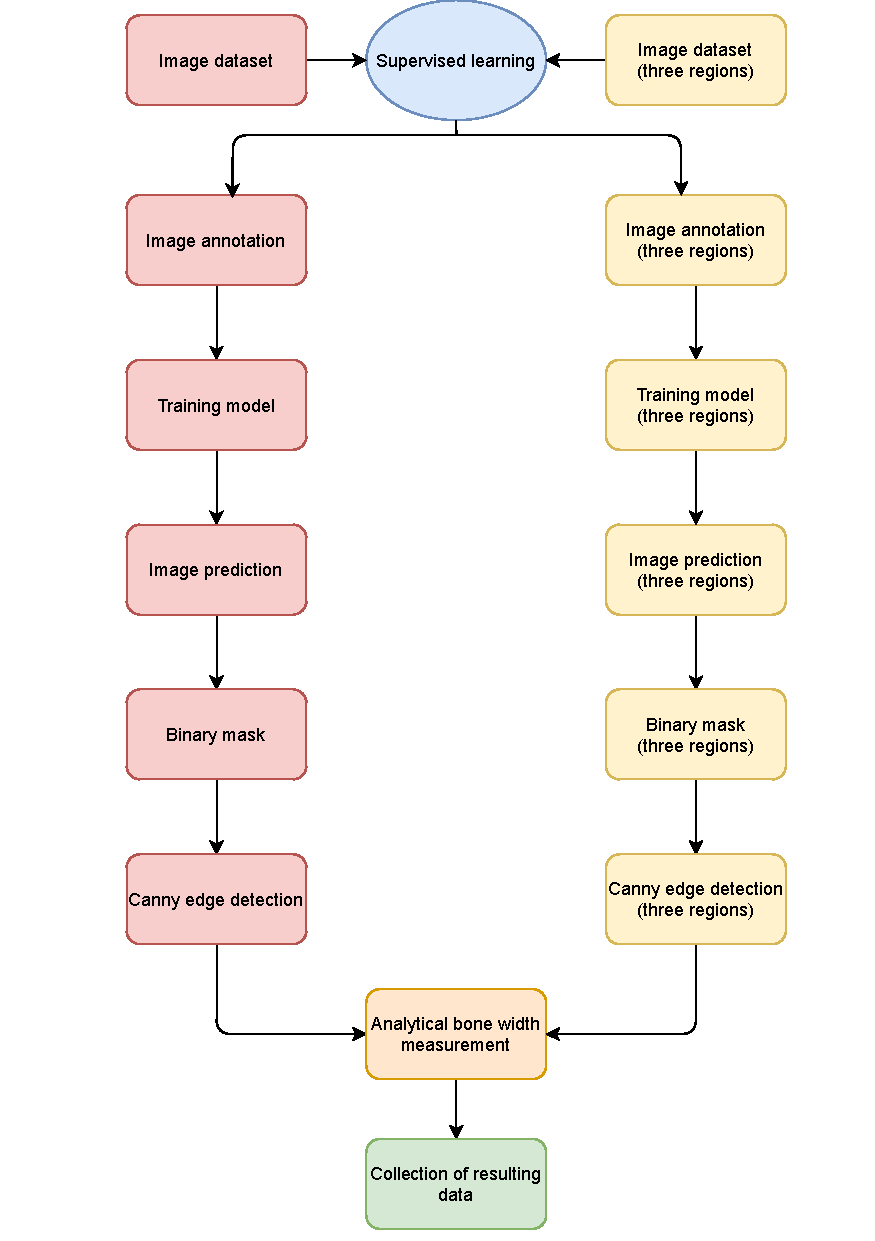
\includegraphics[width=.66\textwidth]{obrazky-figures/successful.pdf}
    \caption{\textbf{Flowchart.} Image shows flowchart for pattern recognition using CNN.}
    \label{flowchart2}
\end{figure}

\begin{figure}[!ht]
    \centering
    \begin{subfigure}[b]{.25\textwidth}
    \centering
        \frame{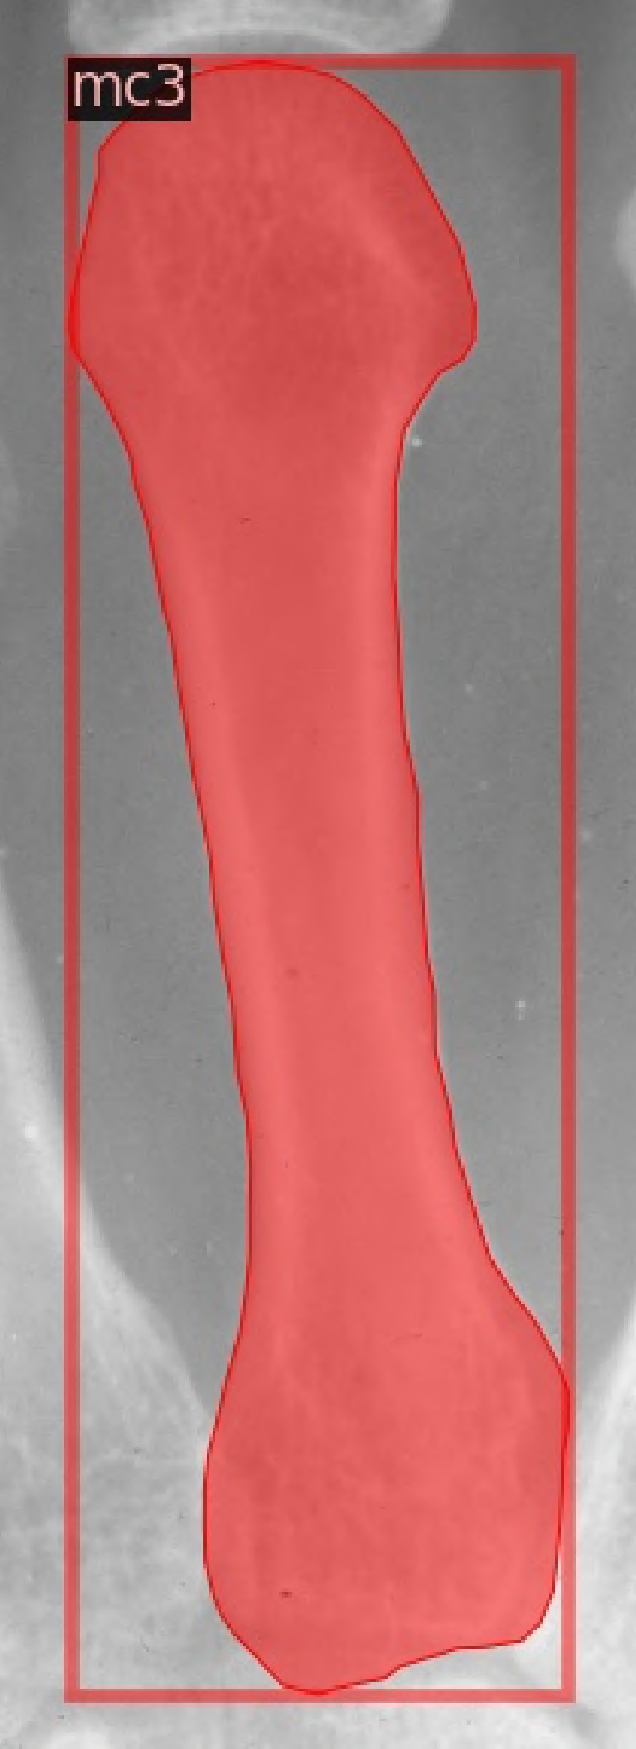
\includegraphics[width=.6\textwidth]{obrazky-figures/GT.pdf}}
        \caption{}\label{GT-img}
    \end{subfigure}
    \begin{subfigure}[b]{.25\textwidth}
    \centering
        \frame{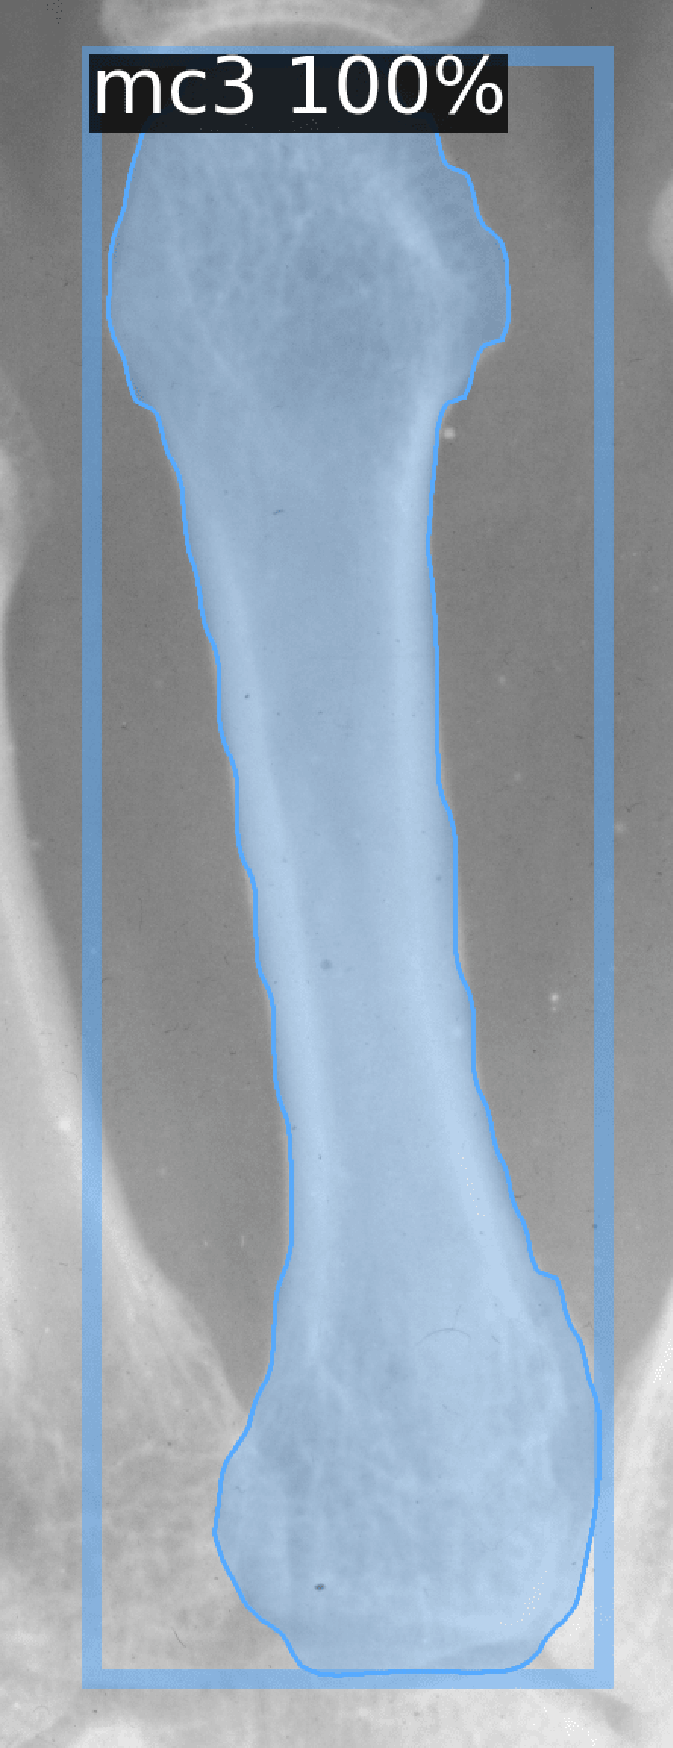
\includegraphics[width=.6\textwidth,height=2.46in]{obrazky-figures/GT_comparission.pdf}}
        \caption{}\label{GT-fake-img}
    \end{subfigure}
    \caption{\textbf{Ground truth comparison.} (a) Ground truth image. (b) Predicted image mask.}
    \label{GT}
\end{figure}

\subsection{Image Conversion to Compatible Format}
In order to annotate the database, it is required to perform an image format conversion. As the result of the X-ray image database being in TIF format, and the selected annotation tool being unable to process images in this format, the images have been converted to JPEG format.

\subsection{LabelMe Annotation}
There are a number of tools for image annotation, and at this point it depends mostly on~the~tools and libraries that are used in the algorithm. From the point~of view of~the~Detectron2 library, which uses the COCO dataset for object detection introduced in paper \cite{coco2015microsoft}, to create an object detection model, it is vital to work with files in a special JSON format called JSON COCO. This is a special format that describes how labels and metadata are stored in the image dataset \cite{COCO-JSON}. Images of count 180 from the X-ray images of~human hand database were used for the image annotation. After thorough communication with the~staff from the anthropological institute, the final annotation was performed by the institute itself due to expertise and accuracy of labeling. X-rays are not always easily recognizable and contain many artifacts and bone overlaps, which often only experienced radiologist are familiar with. Situation is no different with metacarpal bones, and an inexperienced person can often annotate incorrect regions or parts of the bone which it actually does not contain~\cite{labelme}. The  image \ref{annotation} shows the way of how to annotate images.

\begin{figure}[!ht]
    \centering
    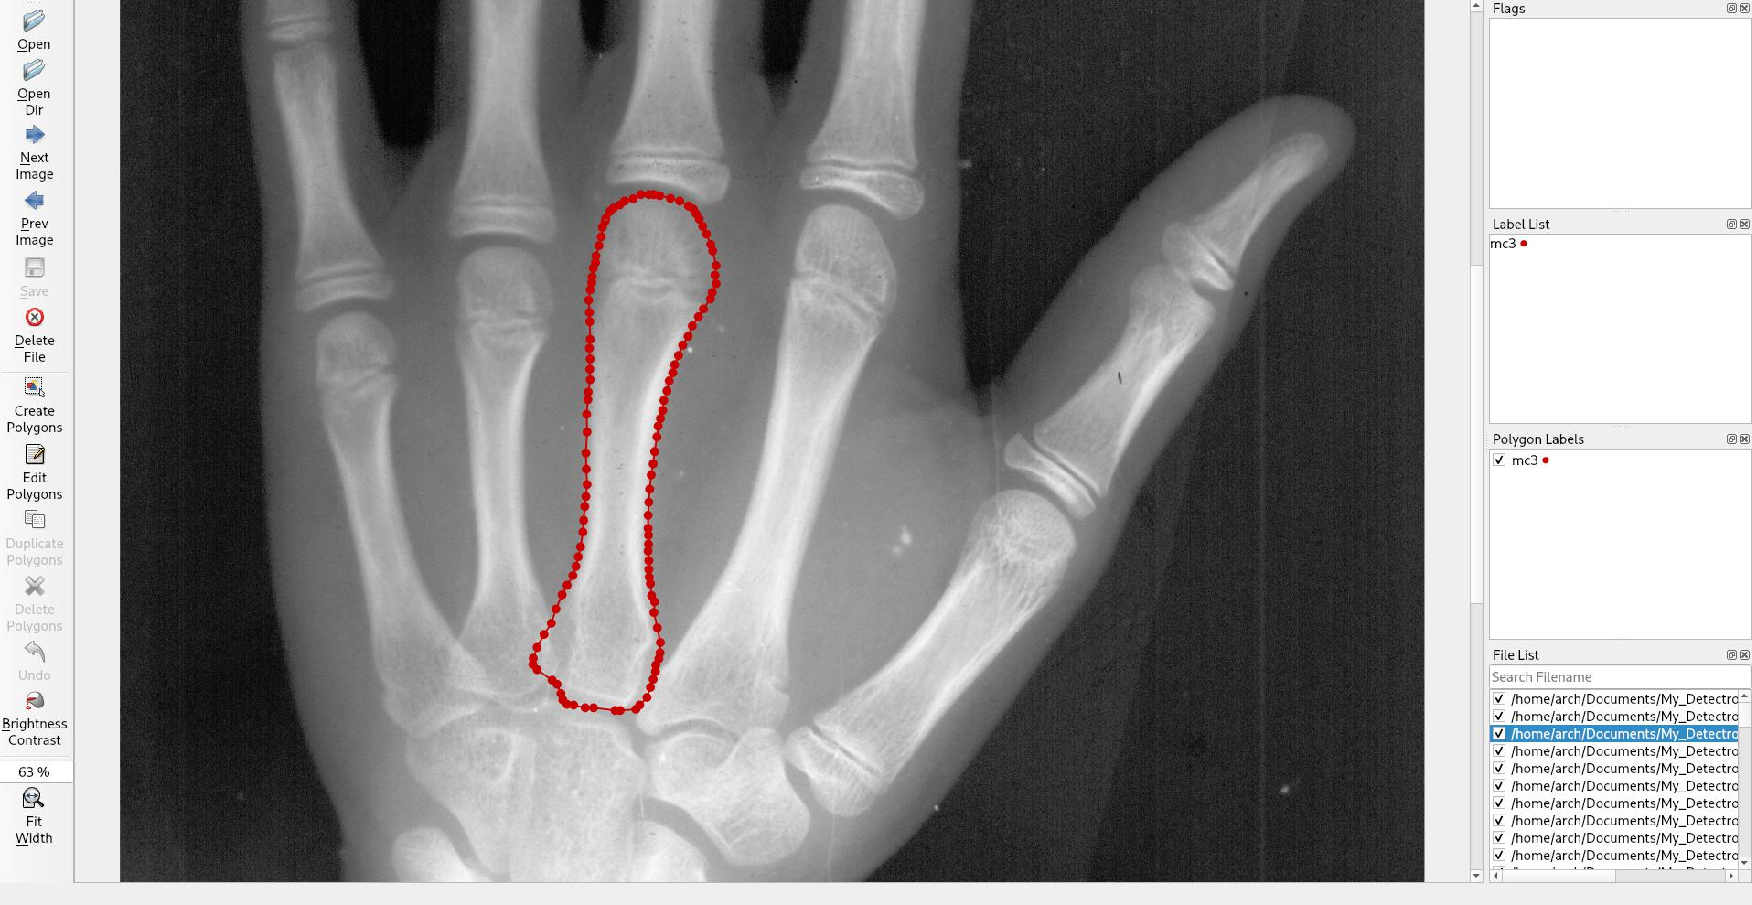
\includegraphics[width=.7\textwidth]{obrazky-figures/annotation.pdf}
    \caption{\textbf{Annotation in LabelMe.} Very precise annotation made by MUNI anthropological institute.}
    \label{annotation}
\end{figure}

\subsubsection*{Conversion to COCO JSON Format}
Annotation tool LabelMe, which creates its own JSON file for each annotated image. After that, the available script called \textit{labelme2coco.py} is used, which facilitates the rest of the~annotation work. In order to be able to create a model for object detection, it is necessary to convert all the~labeled JSON files into a single COCO dataset annotation JSON file which currently provides the mentioned script taken from the work \cite{JSONtoCOCO}.

\subsection{Training Model}
\label{training-model}
After a successful conversion, the training process can be started. Training on annotated images from the X-ray image dataset is performed using the Detectron2 library. The training process itself is not a simple task. It requires a lot of testing and experimentation. In~order to be able to create a model as accurately as possible, it is necessary to work with several parameters that are required when working with neural networks. In addition, the~training process is often very time consuming and depends a lot on the computer resources on which the training is performed. For this reason, the training of the model was performed using Google Colaboratory, which provides quality GPU acceleration \cite{google-colab}. Metrics for model training:
\begin{itemize}
  \item Configuration file: \textbf{mask\textunderscore rcnn\textunderscore R\textunderscore 101\textunderscore FPN\textunderscore 3x.yaml} loading model zoo configuration, using  ResNet and FPN(Feature Pyramid Networks) backbone
  \item Model weights: \textbf{mask\textunderscore rcnn\textunderscore R\textunderscore 101\textunderscore FPN\textunderscore 3x.yaml} loading pre-trained weights based on model zoo from Detectron2 library
  \item Number of iterations: \textbf{10000}
  \item Number of parallel data loading workers: \textbf{2}
  \item Number of images per batch across all machines (depends on number of GPU's): \textbf{2} meaning that each GPU will see two images per batch
  \item Learning rate: \textbf{0.00025} is the hyperparameter that controls how much to change the~model in response to the estimated error each time the model weights are updated, it has big impact for resulting model
  \item Batch size per image: \textbf{128} number of samples or images, that will be propagated through the network
  \item Number of classes: \textbf{1} is the number of detected thing classes in one image
\end{itemize}

During the training and search phase of the most suitable model, many combinations were created to find the most relevant one. The results were empirically researched and manually compared. The output of the training process is a model in PKL format with the name \textit{model\textunderscore final\textunderscore 10k.pth}.

\subsection{Loading Image Dataset}
The algorithm is adapted to be able to load a database of images from a specific directory, including recursively all subdirectories in the image database. This method of reading images is thus designed because the provided database is divided into two subdirectories. These directories are MALES and FEMALES. X-rays were taken from many people over a period of several years and were also differentiated by gender. After loading the image from the dataset, inference, contour detection and analytical measurement of bone width are performed on each of these images.

\subsection{Creating Inference on Image Dataset}
\label{inference}
Creating predictions on images is relatively easy thanks to Detectron2. The principle is based on the use of function \texttt{predict(...)}, which returns several types of predictions such as bounding box coordinates, percentage accuracy of the detected object and mask of~the~predicted object. 

\subsection{Image Binary Mask Creation}
To obtain the contour of the bone, a binary mask of the object must be created. It is one of~the~most important steps, which greatly facilitates the subsequent steps in the~algorithm. Nevertheless, the creation of a binary image of the detected bone does not present a complication from the programming perspective. The code \ref{mask-code}  converts the mask of the~detected object, which is part of the detector from the Detectron2 library and is composed of~the~values \textit{True} or \textit{False}. From these values it creates a binary mask with a range of~0-255 values, where each value of True is assigned the value 255 as white color and vice versa the value of False is assigned a black color with the value 0.

\begin{lstlisting}[label={mask-code}, caption={\textbf{Python code function.} Function for binary mask creation.}]
def binaryMask(mask):
    height = mask.shape[0]
    width = mask.shape[1]
    
    # black image matrix with zero values
    binary_mask = np.zeros((height, width))
    binary_mask += mask

    # binarization of image to values 255 or 0
    for y in range(height):
        for x in range(width):
            # obtaining value of pixel, which can be 0 or 1 (False/True)
            pixel = binary_mask.item(y, x) 
            if pixel:
                binary_mask[y,x] = 255
            else:
                binary_mask[y,x] = 0
    return binary_mask
\end{lstlisting}

The result of the binary mask created in this way can be seen in the image \ref{canny-mask}. The~mentioned function processes each mask of the image separately, which means that in a case that the prediction of object detection has found several bones of the third metacarpus, then each such bone will be processed separately. In most cases, the database contains an~X-ray image of the left hand, but there are some cases where both hands were scanned, which can be seen in the image \ref{LP}.

\begin{figure}[!ht]
    \centering
    \begin{subfigure}[b]{.40\textwidth}
        \frame{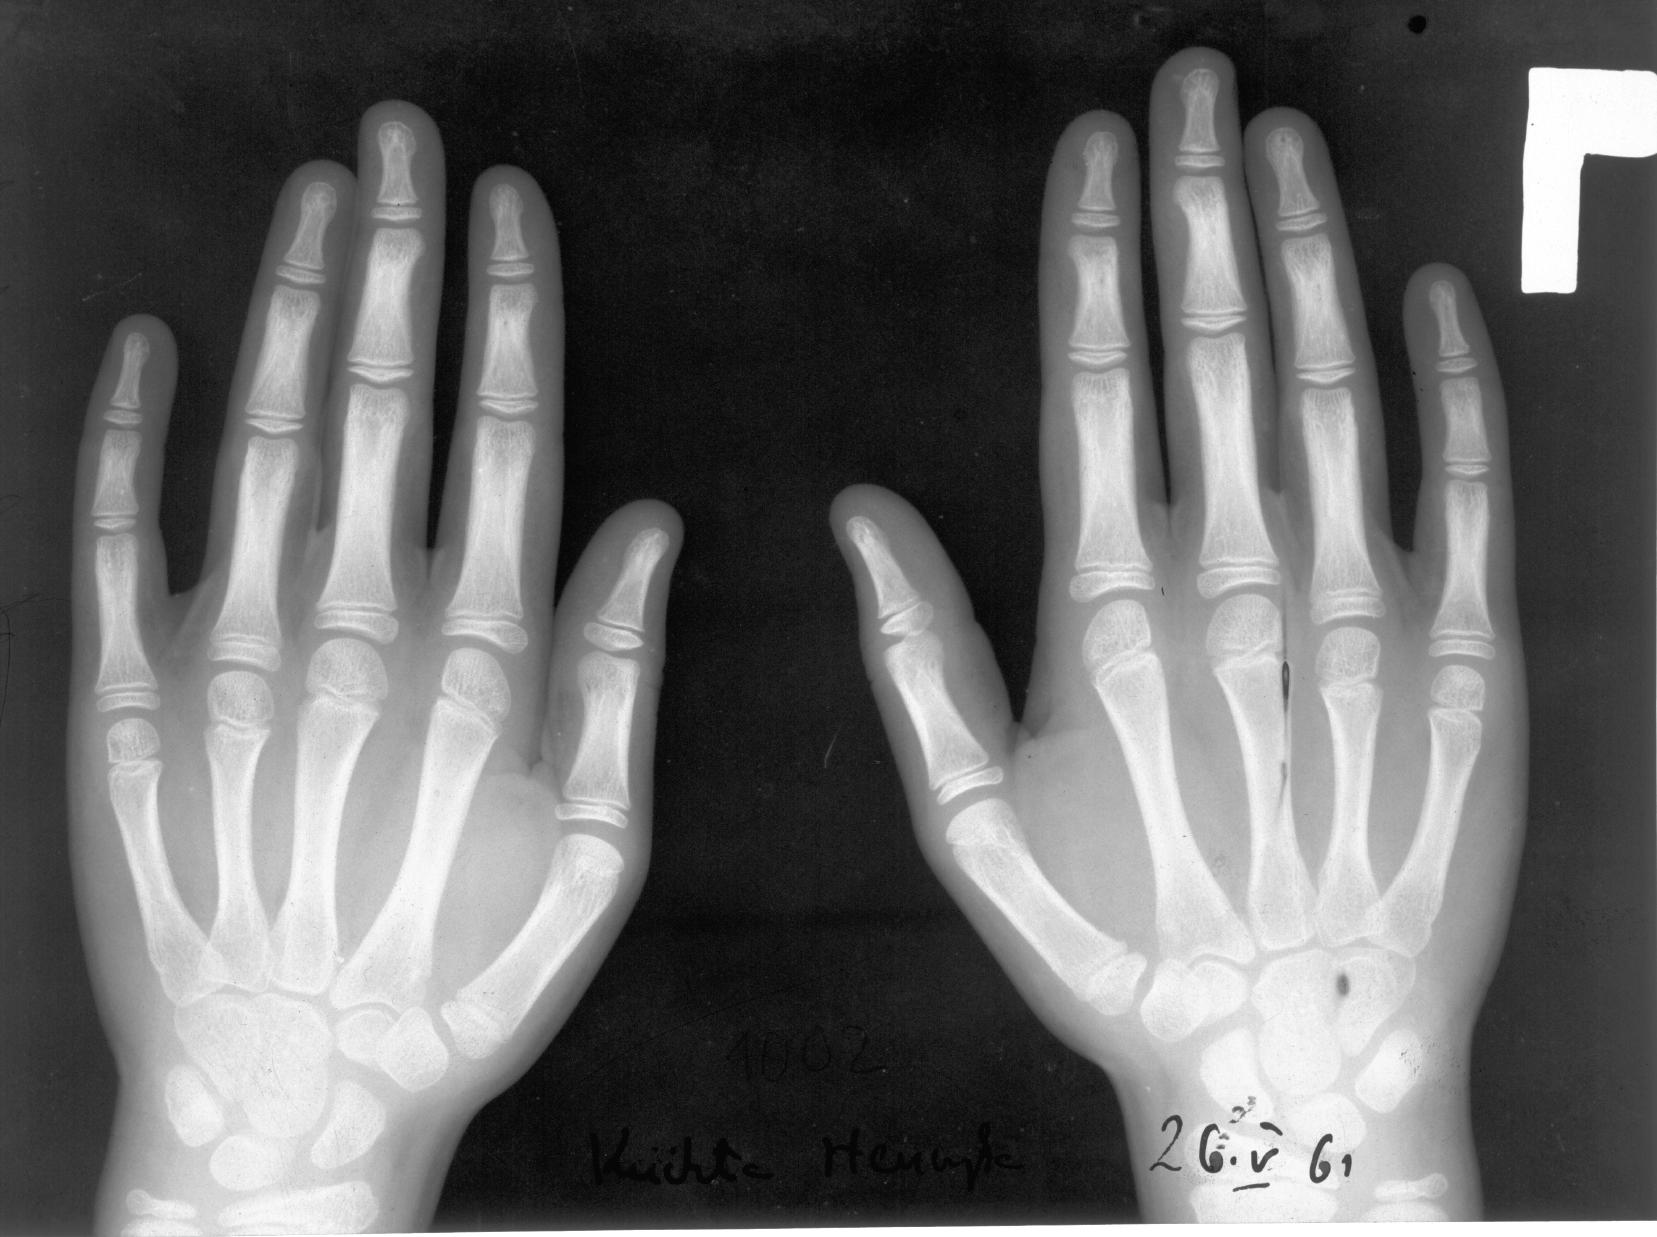
\includegraphics[width=\textwidth]{obrazky-figures/LP.pdf}}
        \caption{}\label{LP-img}
    \end{subfigure}
    \hspace{1em}
    \begin{subfigure}[b]{.40\textwidth}
        \frame{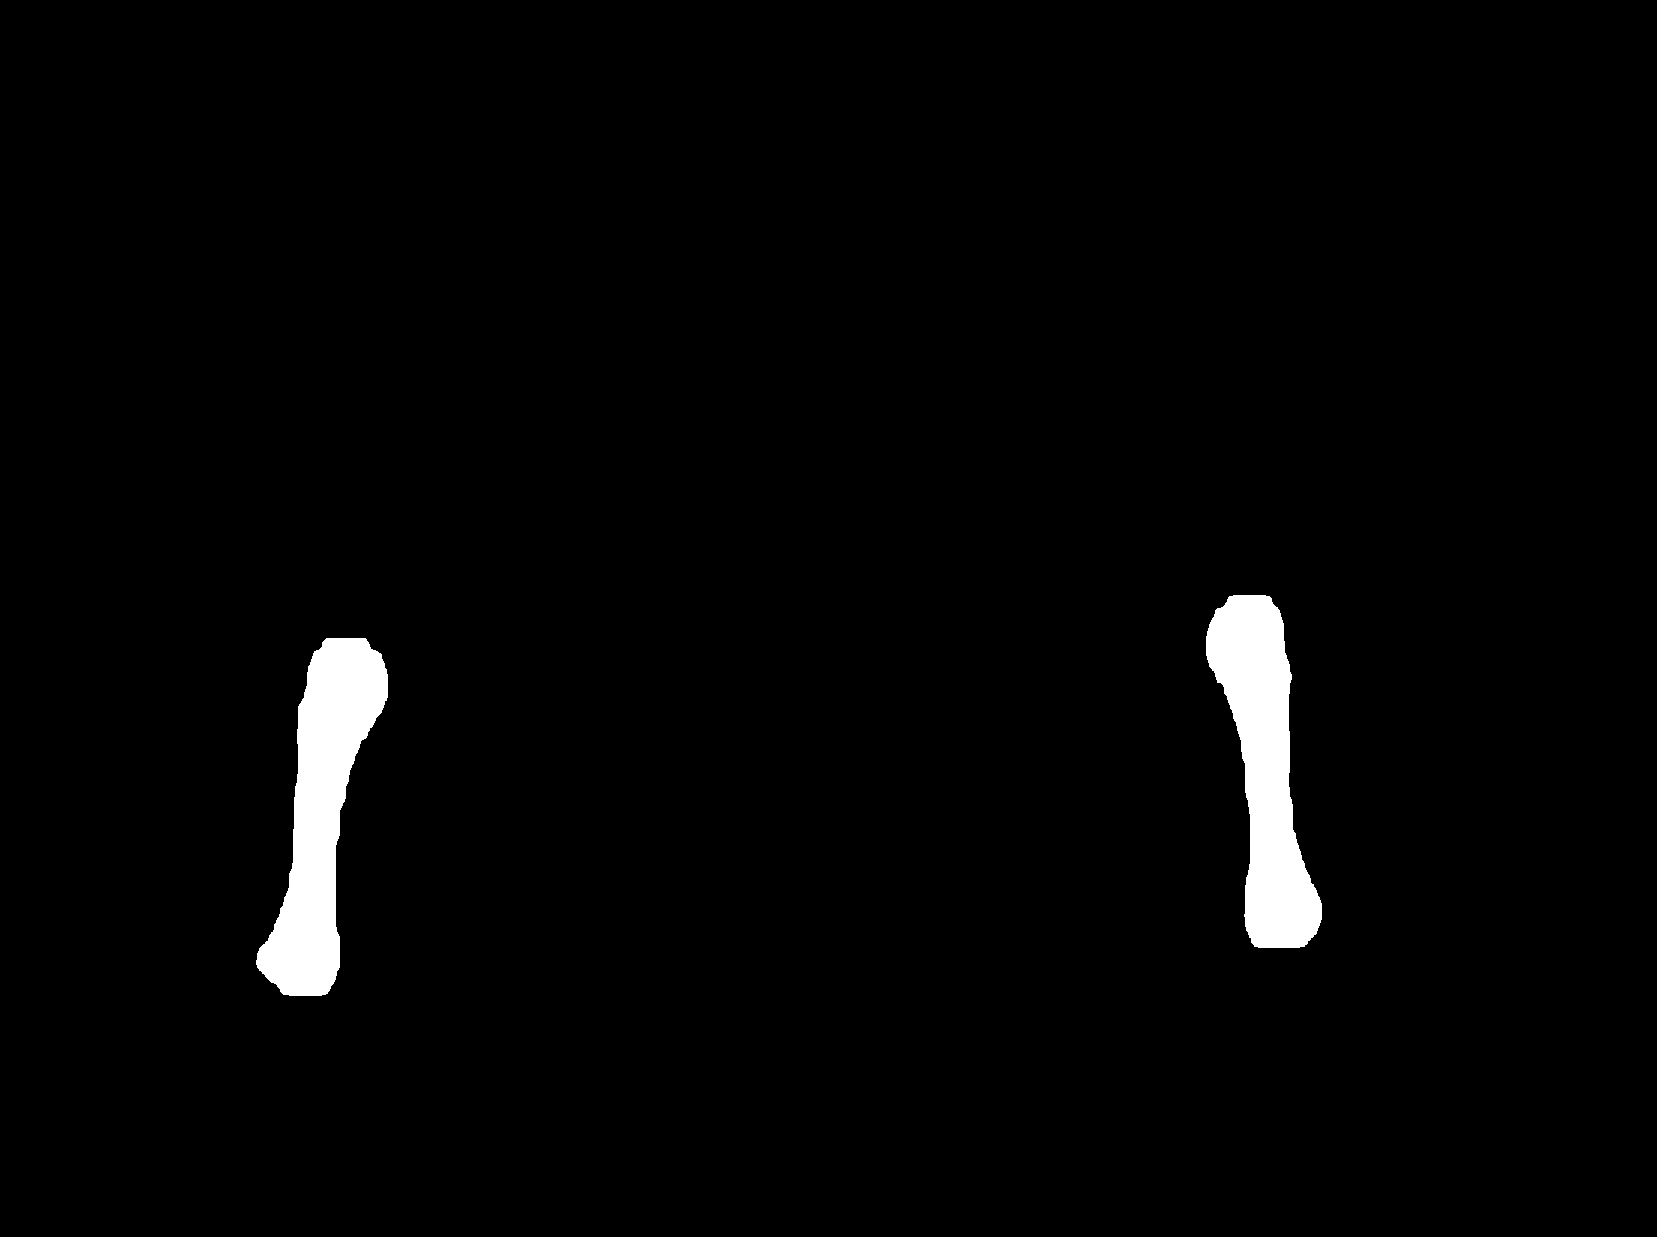
\includegraphics[width=\textwidth]{obrazky-figures/LP_masks.pdf}}
        \caption{}\label{LP-mask-img}
    \end{subfigure}
     \caption{\textbf{X-ray image with both hands and the output mask for the~third metacarpus.} (a) X-ray image. (b) Binary mask.}
    \label{LP}
\end{figure}

\subsection{Contour Creation}
The traditional methods which were described in the beginning of the chapter \ref{chapter3} as unsuitable for segmentation and contour detection, are nevertheless used in this algorithm, in which they have proven to be effective and reliable. The following steps would not be possible without obtaining a binary mask of metacarpal bones using instance segmentation and Mask R-CNN, as this is a critical part of the algorithm. The \texttt {Canny(...)} method from the OpenCV library is used to extract the contour of a bone whose width is perfectly one pixel and at the~same time the bone is fully drawn, which meets all the requirements and works uniform for every image of a binary mask. The output from this part of the~algorithm is in the~image~\ref{canny-contour}.

\subsection{Contour Coordinates Export}
Obtaining coordinates from the bone contour closes the first part of the algorithm, whose task is to detect the contour. In addition to the outputs of the algorithm in the form of~images, which are stored in individual directories, the outputs are also text files. This~step was designed following the preferences of people from the anthropological institute, whose recommendations were outputs in TPS format. In TPS format, each image has its own file with the name of the bone, which contains the contour coordinates of each detected bone in the format \texttt {[x,y]}.

\subsection{Analytical Bone Width Measurement}
The second part of the algorithm is the analytical measurement of the width of the third metacarpal bone. This part of the program does not use any of the methods for pattern recognition and computer vision. Analytically, the measurement approach works primarily with individual pixel coordinates by comparing their mutual distances. The task is not simple and is relatively computationally demanding, as the images from the database are in high resolution and iterations through the image matrix are quite time-consuming.

\subsubsection*{Bone Center Line Approximation}
Approximation of the center line of the bone is the most important, and also the most difficult task for finding the distance. Since it is possible to compare the distances of~each pixel from the left side of the bone with each pixel on the right side, it is essential to~divide the bone into two parts. The most relevant way to perform this division is by using the~center line approximation. Since the bone is not a symmetrical shape, it is necessary to find a center line in an irregular polygon. This requires the connection of two points. These points are then used to divide bone into two as symmetrical halves as possible.

In the section \ref{inference}, it is mentioned that in addition to the bone mask of Detectron2, the~coordinates of the predicted bounding rectangle are also obtained. These are two points, the~coordinates of which are the point \texttt{P1[topleft\textunderscore x, topleft\textunderscore y]} and the point \texttt{P2[bottomright\textunderscore x, bottomright\textunderscore y]}. These coordinates are in the algorithm necessarily for the approximation of the center line. The function \texttt{middleX(...)}, the code of which can be seen in \ref{middle-x-code}, is used for the approximation of~the~middle X coordinate by arithmetic mean. This X coordinate is calculated for both top and bottom of the bone. It uses the coordinates of points from the bounding rectangle. After calculating the middle X coordinates, the bone can be easily divided into two parts using the center line. The bone image is shown in the \ref{center-line} image.

\begin{lstlisting}[label={middle-x-code}, caption={\textbf{Python code function.} Function of middle x coordinate approximation for center line.}]
def middleX(top_or_bottom_y,bottomright_x,topleft_x,offset,img):
    height = img.shape[0]
    width = img.shape[1]
    x_coords = list()

    for i in range(offset):
        for y in range(height):
            for x in range(width):
                if x >= topleft_x and x <= bottomright_x:
                    # detecting pixels from the top left or bottom right y 
                    # coordinate on the way up
                    if y == top_or_bottom_y - i:
                        if img[y,x] == 255: # edge found
                            x_coords.append(x)
                    # detecting pixels from the top left or bottom right y 
                    # coordinate on the way down
                    if y == top_or_bottom_y + i + 1:
                        if img[y,x] == 255: # edge found
                            x_coords.append(x)
                            
    # mean average from all x coordinates found
    avg_x = np.mean(x_coords)
    
    # middle x coordinate
    return round(avg_x) 
\end{lstlisting}

Since bone structure is often irregular and the prediction of the location of the bone vertices is not possible, it is necessary to collect X coordinates from~the top or bottom of~the~bone. The top or bottom of the~bone may contain various local maxima or minima, and if the~diameter X of the coordinates were formed only in the range of one pixel of the Y coordinates, this would often lead to false and inaccurate conclusions of the~approximation of~the~middle X coordinate. Therefore, an offset is used in the algorithm, which is set to the empirically tested magic number 40. This number means that all X coordinates from the range of~40 pixels of Y coordinates are taken, and they are used to calculate the~mean average. In~such laborious and computationally demanding way, which requires a~lot of iterations, it is possible to approximate with sufficient precision where the middle X coordinate will be located.

\begin{figure}[!ht]
    \centering
    \frame{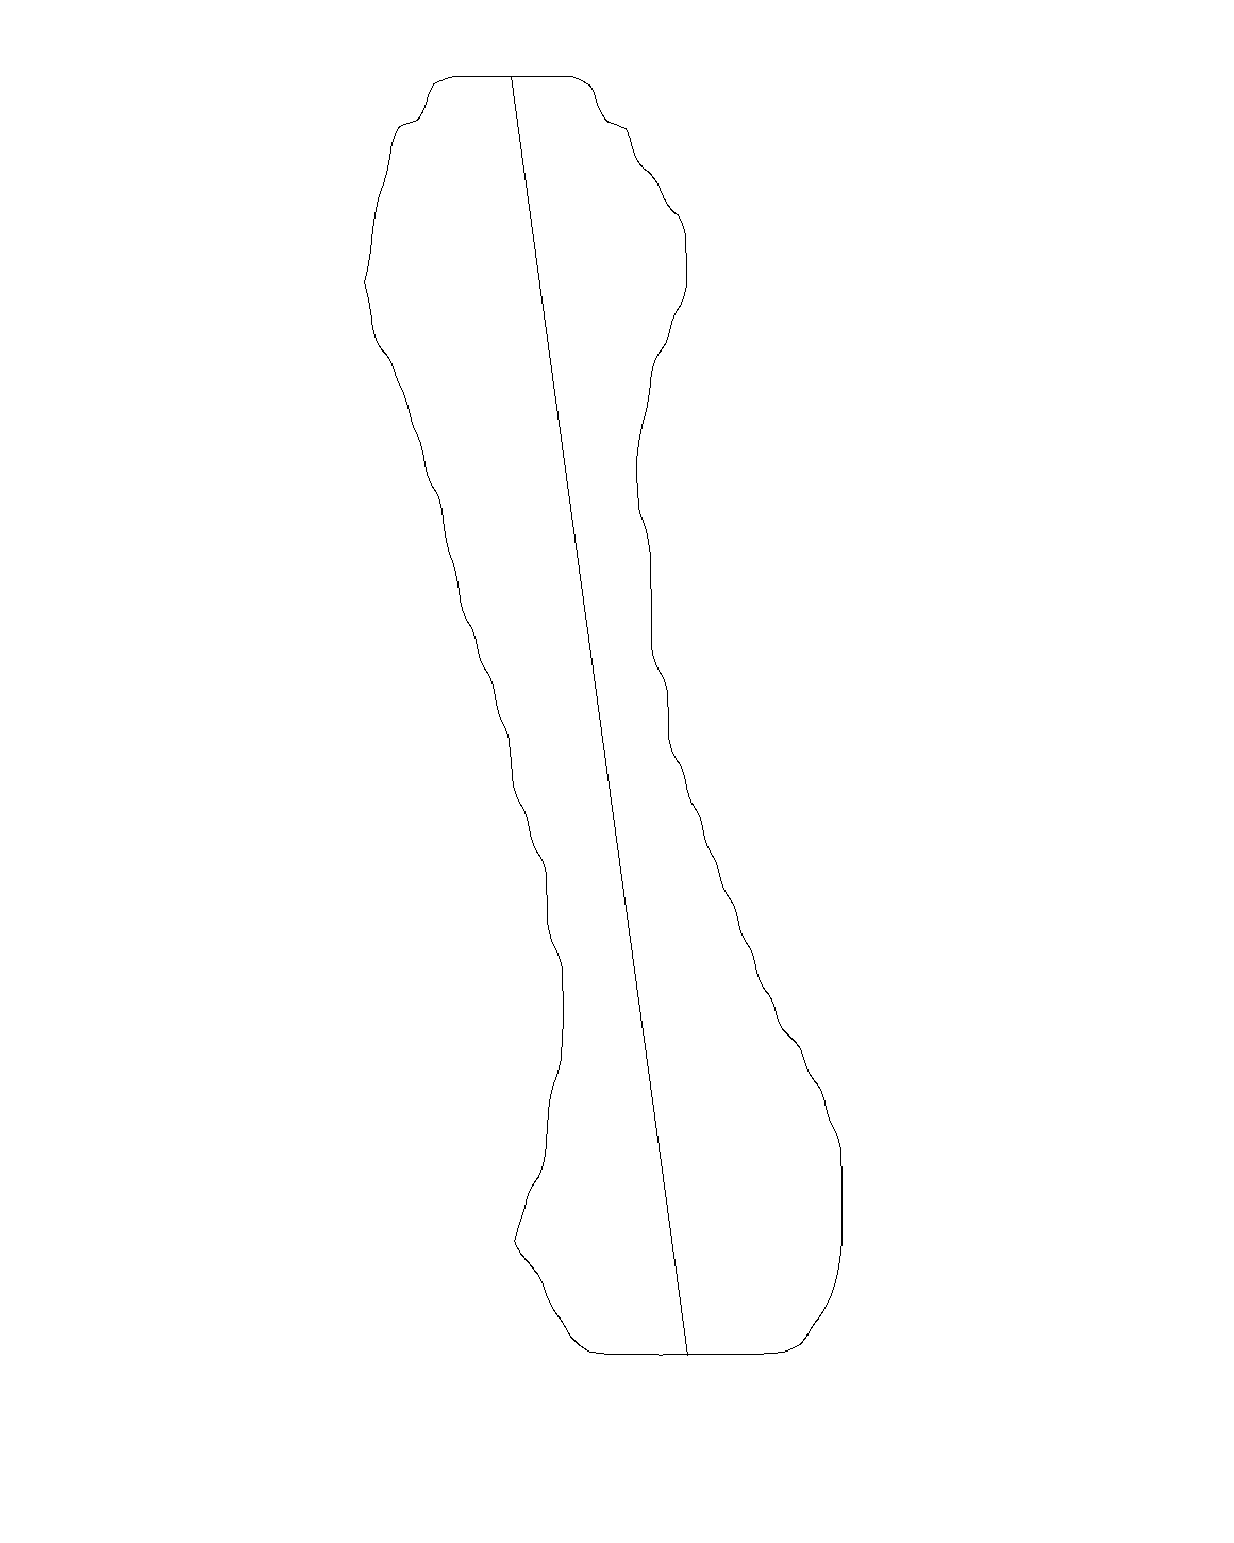
\includegraphics[width=.5\textwidth]{obrazky-figures/full_with_center_line.pdf}}
    \caption{\textbf{Bone with center line.} Image shows approximated center line using two points with computed middle X coordinate.}
    \label{center-line}
\end{figure}


\subsubsection*{Bone Division}
To calculate the distance between two points of the left part of the bone and the right part of the bone, it must be determined which of the points will belong to the right and left side. To do this, there is used the obtained center line of the bone. In order to decide whether a given point can be found on the right or left side, the task is to determine whether a~given point lies below or above the given abscissa, which forms the center line of the bone. According to \cite{cross-product-isabove}, it is possible to use a cross product as a decision threshold. Therefore, in the case of this algorithm, the following must apply \cite{cross-product-equation}:
\begin{equation}
\begin{split}
A &= (x_1,y_1)\\
B &= (x_2,y_2)\\
P &= (x,y)\\
d &= (x - x_1)(y_2 - y_1) - (y - y_1)(x_2 - x_1)
\end{split}
\end{equation}
In this equation must hold that if \(d <0 \), then the point \textit{P} lies above the line or on the left side, otherwise the point lies on the opposite side. Points \textit{A} and \textit{B} create the center line.
\begin{lstlisting}[label={bone-division-code}, caption={\textbf{Python code function.} Function divides bone into two halves using center line.}]
def divide(topleft_x,topleft_y,bottomright_x,bottomright_y,offset,img):
        left_side = list()
        right_side = list()
        
        # lambda expression for point location 
        # determination returns True or False
        cross_product_isabove = lambda p3,p1,p2: np.cross(p3-p1, p2-p1) < 0
    
        # center line points
        p1 = np.array([topleft_x,topleft_y])
        p2 = np.array([bottomright_x,bottomright_y])
        
        # image shape
        height = img.shape[0]
        width = img.shape[1]

        for y in range(height):
            for x in range(width):
                if y >= topleft_y + offset and y <= bottomright_y - offset:
                    if img[y,x] == 255:
                        p3 = np.array([x,y])
                        if cross_product_isabove(p3, p1, p2):
                            left_side.append([y,x])
                        else:
                            right_side.append([y,x])

        return left_side, right_side
\end{lstlisting}

It is important to realize that in order to obtain relevant points for both left and right side, the distance between two points, whether on the head or the base of the bone, must not be taken into account. Since the goal is to find the distance in the narrowest part of~the bone from the anthropological point of view, and thus from the point of view of~bone structure, it~will certainly not be located on the head or base of the bone but will be located in the~body of the bone. However, from the~computer algorithm point of~view, this fact should be included in the calculation. Otherwise, the shortest distance will be found between two points, where the center line divides the bone into two halves and not in the middle of the~bone. For this reason, there is an empirically chosen magic offset in~the~algorithm, which arranges that the distance starts to be calculated only after omitting a~certain number of~pixels in the y-axis, and this applies to head and base as well. This magic constant is chosen to be 150, which works well for all the bones of the third metacarpus. In~the~image \ref{left-right-side}, it is possible to see the division of the bone into right and left side. In~images \ref{left-side} and \ref{right-side}, the offset of 150 pixels is neglected for clarity.

\begin{figure}[!ht]
    \centering
    \begin{subfigure}[b]{.45\linewidth}
        \frame{
\includegraphics[width=\linewidth, height=3in]{obrazky-figures/left_side.pdf}}
        \caption{}\label{left-side}
    \end{subfigure}
    \hspace{1em}
    \begin{subfigure}[b]{.45\linewidth}
        \frame{
\includegraphics[width=\linewidth, height=3in]{obrazky-figures/right_side.pdf}}
        \caption{}\label{right-side}
    \end{subfigure}
     \caption{\textbf{Images show the bone division according to center line.} (a) Left side of the bone. (b) Right side of the bone.}
    \label{left-right-side}
\end{figure}

\subsubsection*{Finding Minimal Distance Using Pythagoras Theorem}
The final measurement of the distance between two points \textit{A} and \textit{B} is no longer a difficult task. Sequentially, each distance of the left side of the bone will be compared with the right side of the bone. To find this distance, Pythagoras theorem is used, where the following holds:
\begin{equation}
\begin{split}
A &= (x_1,y_1)\\
B &= (x_2,y_2)\\
distance &=\sqrt{(x_1 - x_2)^2 + (y_1 - y_2)^2}
\end{split}
\end{equation}
If the new distance is less than the distance measured for the previous two points, it becomes a new minimum distance. The image \ref{center-line-width} shows the final result of the analytical approach, which includes the center line, minimal length that was found, and the bone contour itself, which does not include the head and base of the bone.

\begin{figure}[!ht]
    \centering
    \frame{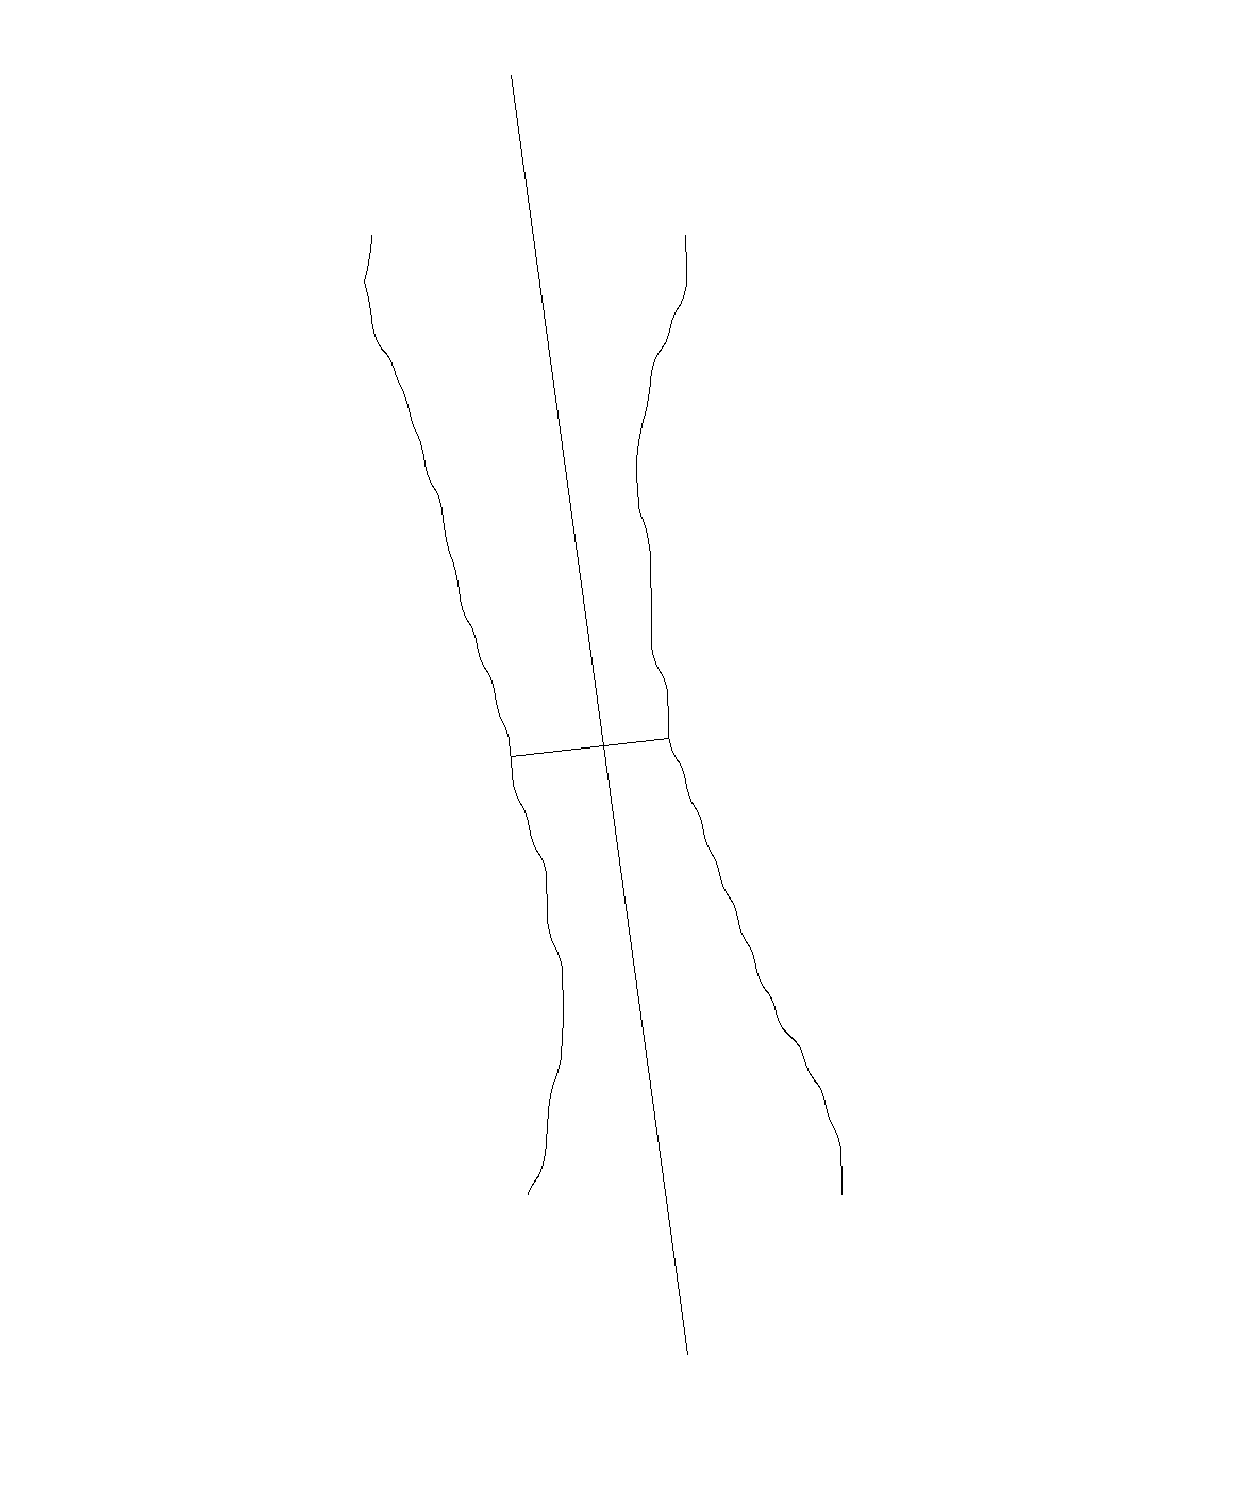
\includegraphics[width=4in,height=4in]{obrazky-figures/full_with_length_and_center_line.pdf}}
    \caption{\textbf{Analytical approach pictured.} Image shows the final minimal length found in the third metacarpal bone.}
    \label{center-line-width}
\end{figure}

\subsubsection*{Pixels Conversion to Millimeters}
Since the measured distances work unequivocally with pixel coordinates, such output would be irrelevant for real research from anthropological point of view. That is why it is necessary to convert such values into actual units of distance. The basic equation is used for the~conversion, but it must be slightly modified. Since the images were made by an anthropological institute, and were rescanned from the material images, it was necessary to find out what DPI(Dots per inch) digital images disposed. The properties of the images themselves provided an indication of 150, which is a relatively standard DPI for higher resolution digital images. However, when the scanning of images was provided, zoom was used and applied to 300\%. This makes the total DPI value a triple and that equals 450. This information was verified and confirmed during communication with anthropology department. The final equation is therefore as follows:
\begin{equation}
\begin{split}
d = \frac{p * c}{DPI} 
\end{split}
\end{equation}
Variable \textit{d} is the final distance in millimeters, \textit{p} is the measured distance in pixels, \textit{c} is a~constant with a value of 25.4 which is the distance of one inch in millimeters and finally \textit{DPI} is a~constant indicating the number of points at a distance of one inch set to 450.

\subsection{Bone Circumference Export}
The results of the measured distances are exported to a file in CSV format, where the~resulting distance in millimeters is given for each image. If the algorithm detected more than one metacarpal bone in the X-ray, these bones are incrementally labeled from the number one.

\subsection{Collection of Resulting Data}
Successfully achieved measurements must be collected in order to enable the interpretation of the algorithm output in the most comfortable way and also to allow more detailed analysis and future work with the collected data for Masaryk University staff, for whom the program output is valuable and created in accordance with their research. At the same time, it is necessary to consider that the measurement results are primarily intended for people who are not so familiar with all kinds of file formats. Therefore, two types of files are used -~TPS and CSV.

In addition to text files with measurements or contour coordinates, the program also saves image outputs during all steps of the algorithm. These outputs include the mask of the~detected bone, the binary mask, the contour acquired using the Canny edge detector and the~resulting image in which a line is drawn in the area of the bone where the shortest distance was measured, as can be seen in the image \ref{detectron-full-width}.

\begin{figure}[!ht]
    \centering
    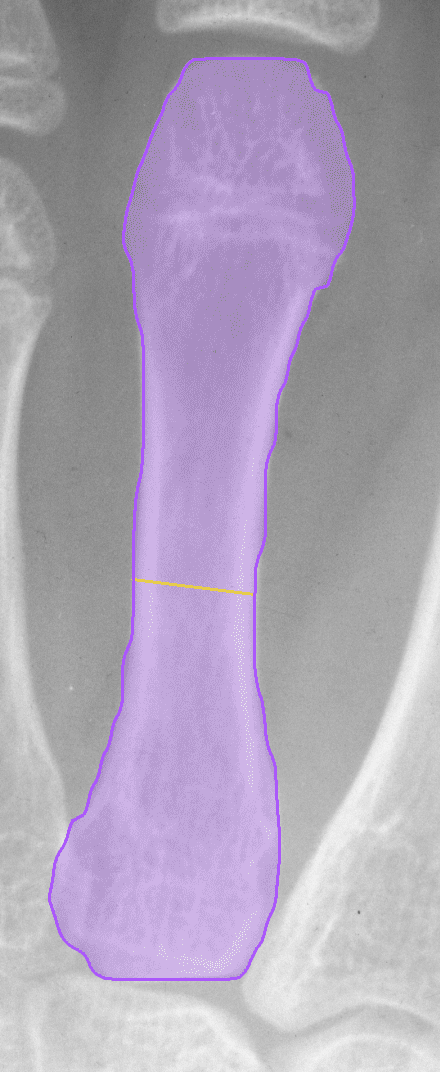
\includegraphics[width=.25\textwidth]{obrazky-figures/detectron_with_full_width.png}
     \caption{\textbf{Minimal length displayed in picture.} Yellow line in the image that shows the minimal length found.}
    \label{detectron-full-width}
\end{figure}

\subsubsection*{Data Text Interpretation}
Based upon communication with the team from Masaryk University, the most suitable way for them to interpret the text data of the obtained coordinates is to use TPS format, which they commonly use in their research. The CSV format will be used to export the~measured distances for each image. This format is also one of the agreed forms of output with the~anthropological institute.

%%%%%%%%%%%%%%%%%%%%%%%%%%%%%%%%%%%%%%%%%%%%%%%%%%%%%%%%%%%%%%%%%%%%%%%%%%%%%%%%%%%%%%%%%%%%%%%%%%%%%%%%%%%%
\section{Advanced Algorithm Extension}
\label{extenstion-design}
This section is an addition of the section \ref{cnn-design}, which describes the extension of the basic algorithm. During communication with the anthropological institute, the ultimate conclusion was made, saying that the algorithm could be improved, and thus the possibilities of~examining metacarpal bones from X-ray images would be extended. The section \ref{tmb-structure}, which thoroughly describes the structure of metacarpal bone, states that long bones are formed by compact bones, which form the edges of the bone, and the so-called medullary cavity that fills the inner bone.

The purpose of this extension is to measure the smallest distance in each of these parts separately, but it must still be in the part where the total distance of the bone width is the~shortest. The approach in this extension will be very similar, despite a certain difference from the basic part of the algorithm. The Detectron2 library is again used to distinguish these three special parts to create a model in the same way as the model for detecting the~mask of the third metacarpal bone. The image \ref{roi-annotation} shows the annotation of the region of interest. The created model consists of three individual classes for each part of the bone separately.

\begin{figure}[!ht]
    \centering
    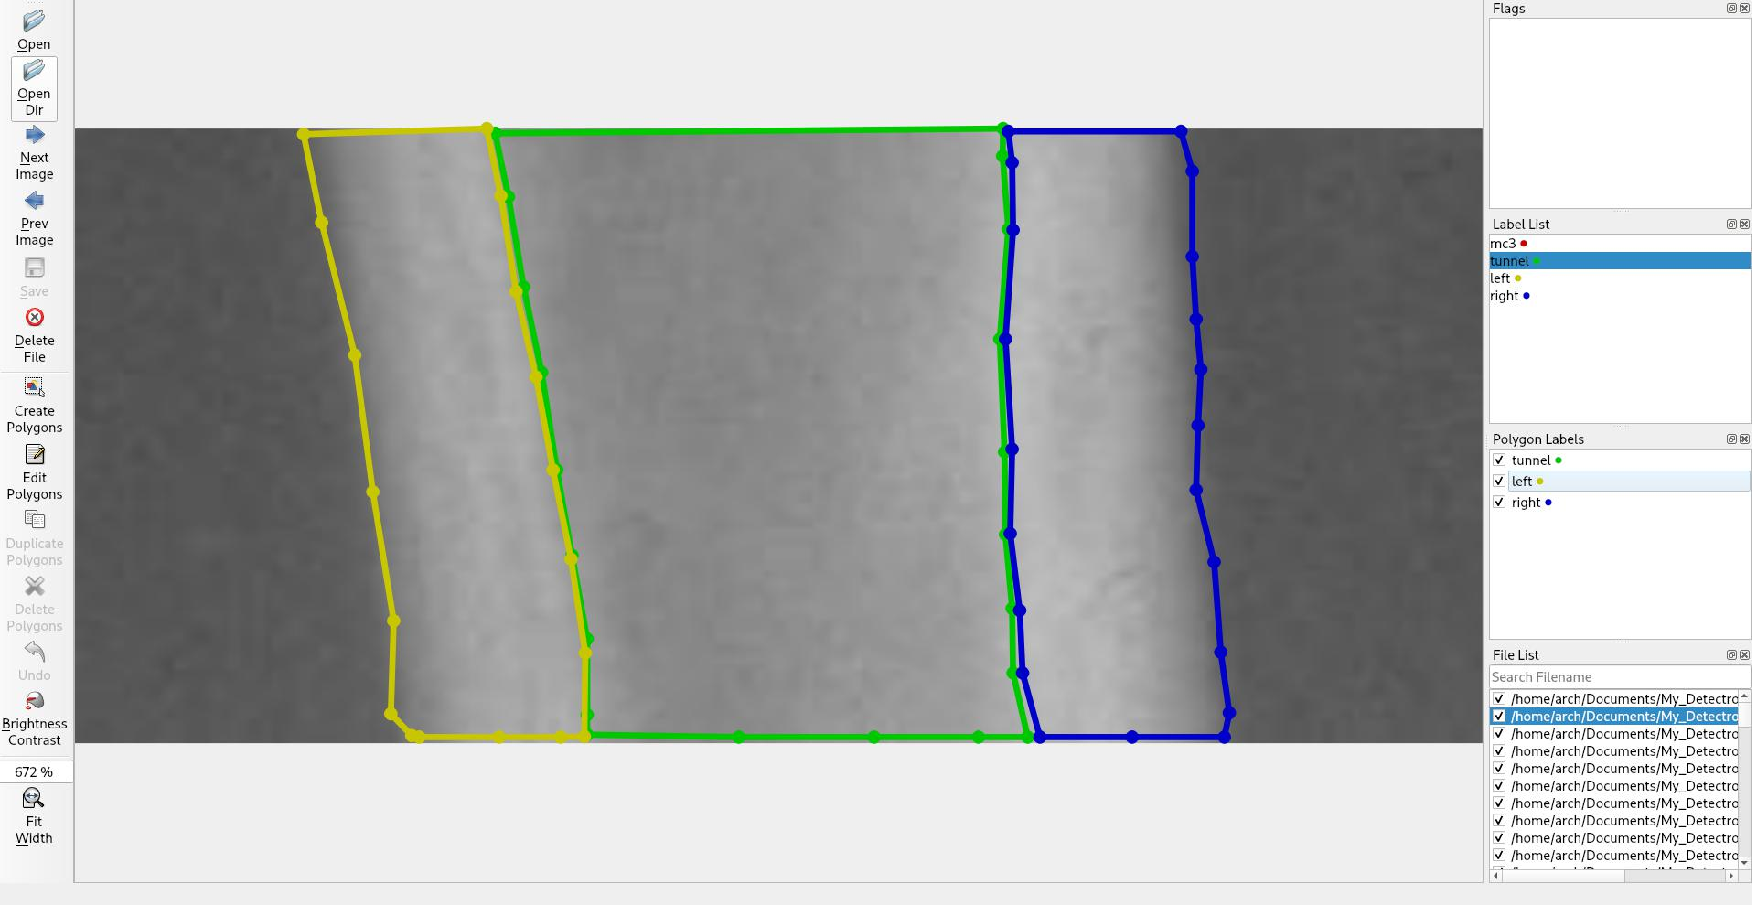
\includegraphics[width=.75\textwidth]{obrazky-figures/ROI_annotation.pdf}
     \caption{\textbf{Annotation of region of interest in LabelMe.} Image shows annotation process for three separate regions of metacarpal bone.}
    \label{roi-annotation}
\end{figure}

\subsection{Model Creation for ROI}
The training process was performed similarly as in the section \ref{training-model}. The chosen metrics for the resulting model are slightly different, but still very similar, thanks to which the~functional model was created. Metrics for model training:
\begin{itemize}
  \item Configuration file: \textbf{mask\textunderscore rcnn\textunderscore R\textunderscore 101\textunderscore FPN\textunderscore 3x.yaml}
  \item Model weights: \textbf{mask\textunderscore rcnn\textunderscore R\textunderscore 101\textunderscore FPN\textunderscore 3x.yaml}
  \item Number of iterations: \textbf{10000}
  \item Number of parallel data loading workers: \textbf{4}
  \item Number of images per batch across all machines: \textbf{2}
  \item Learning rate: \textbf{0.00025}
  \item Batch size per image: \textbf{128}
  \item Number of classes: \textbf{3}
\end{itemize}

\subsection{Bone Measurement in Three Separate Regions}
The created model is similarly utilized, and using the Detectron2 library, a prediction is applied, which creates a mask for each of the regions, which is shown in the image \ref{Detectron2-ROI-inference}. From these masks, a binary mask is then created using the function \ref{mask-code} for each region individually, as can be seen in the image \ref{One-Mask-ROI}. The figure \ref{Mask-ROI} is for illustrating the~binary mask of all three regions in one image. Similarly, an edge detector is applied to these masks using the Canny edge method, where the final output is shown in the figure \ref{One-Canny-ROI}. %The~image \ref{Canny-ROI} is employed again to illustrate what the edge detection would look like if applied to all regions at once. However, this procedure is not used in the algorithm, as the edge detector must be applied separately for each of the detected masks.

\begin{figure}[ht]
    \centering
    \begin{subfigure}[b]{.40\linewidth}
    \centering
       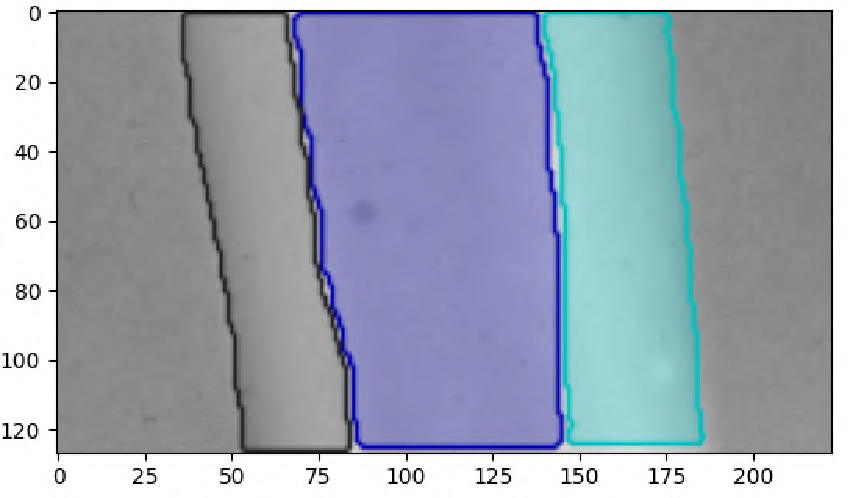
\includegraphics[width=\linewidth, height=2in]{obrazky-figures/3regiony_segmenty.pdf}
        \caption{}\label{Detectron2-ROI-inference}
    \end{subfigure}
    \hspace{1em}
    \begin{subfigure}[b]{.40\linewidth}
    \centering
       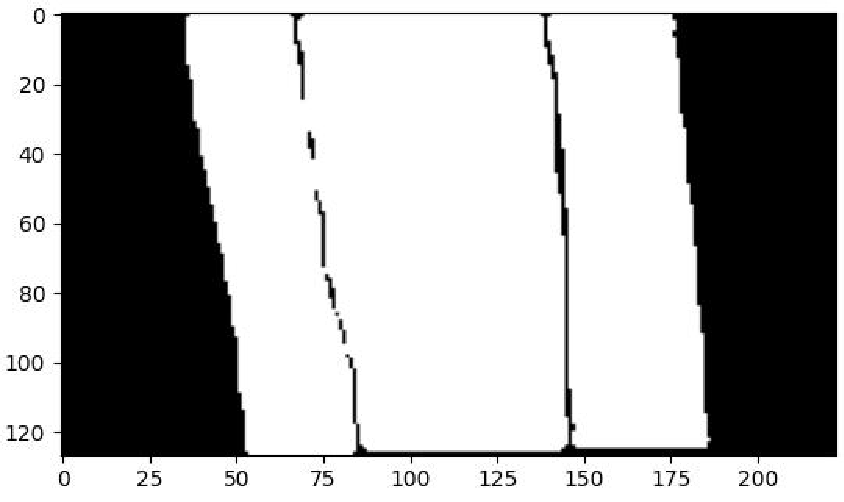
\includegraphics[width=\linewidth, height=2in]{obrazky-figures/ROI_full_mask.pdf}
        \caption{}\label{Mask-ROI}
    \end{subfigure}\ContinuedFloat
    % \begin{subfigure}[b]{.40\linewidth}
    %     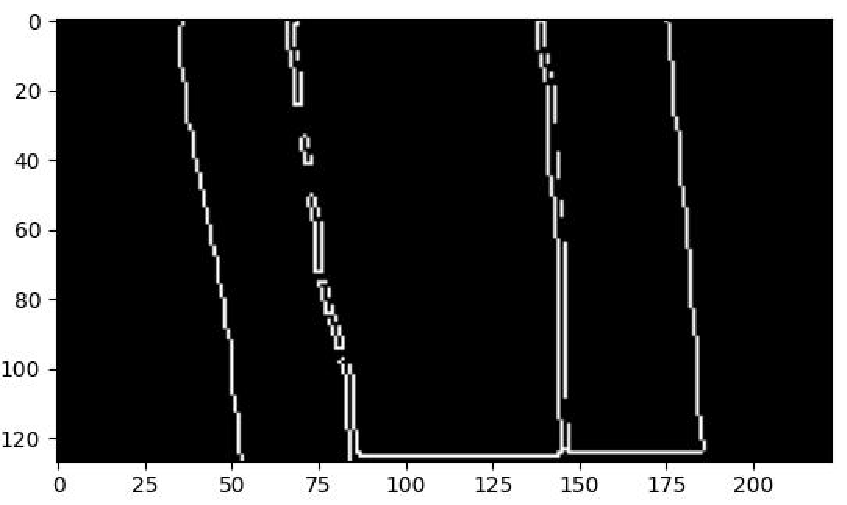
\includegraphics[width=\linewidth, height=2in]{obrazky-figures/ROI_full_canny.pdf}
    %     \caption{}\label{Canny-ROI}
    % \end{subfigure}
    
    \begin{subfigure}[b]{.40\linewidth}
    \centering
        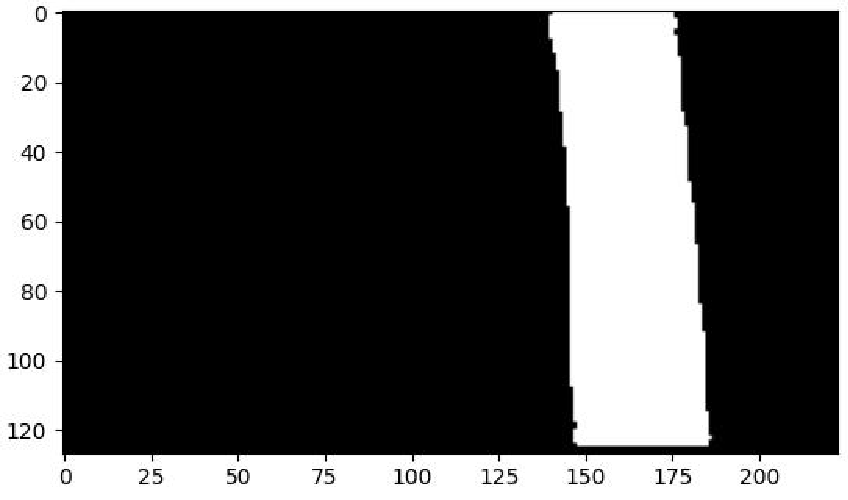
\includegraphics[width=\linewidth, height=2in]{obrazky-figures/ROI_one_mask.pdf}
        \caption{}\label{One-Mask-ROI}
    \end{subfigure}
    \hspace{1em}
     \begin{subfigure}[b]{.40\linewidth}
     \centering
        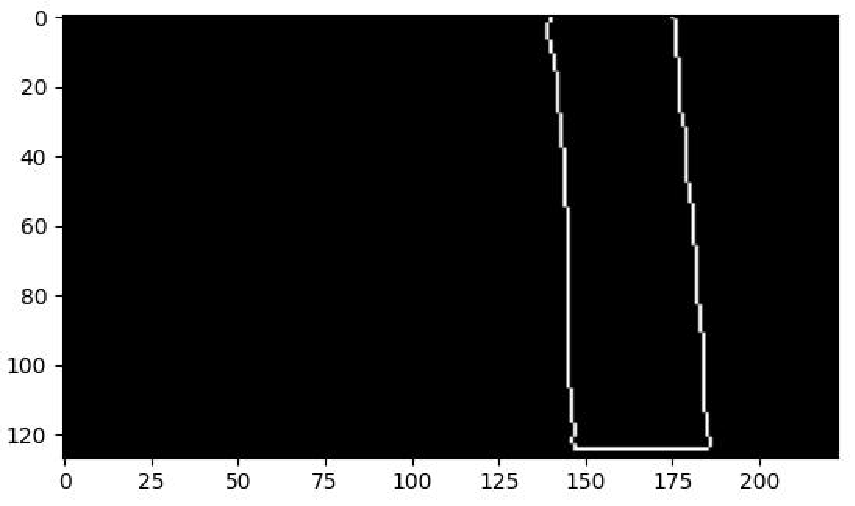
\includegraphics[width=\linewidth, height=2in]{obrazky-figures/ROI_one_canny.pdf}
        \caption{}\label{One-Canny-ROI}
    \end{subfigure}
    \label{ROI-inference}
    \caption{\textbf{Images depicting outputs from extended algorithm for ROI} (a) Detectron2 image mask prediction. (b) Binary mask of predicted image. (c) Binary mask for one of the three segments. (d) Canny edge detector output for applied for one of the three segments.}
\end{figure}


\subsubsection*{Analytical Measurement Approach}
Measuring bone distance is identical to measuring width for the whole metacarpal bone. The~difference is that each of the detected regions is measured individually, which means that the sum of these three distances may not be equivalent to the total distance. If~the~two points that determine the width of the bone do not lie at the same height, which means that the coordinates \(y_1\neq y_2 \), then the range of coordinates in which the~width will be measured in the individual regions is the difference of these coordinates. Therefore, it must hold from $range = \abs{y_1 - y_2}$. The image \ref{measures-comparision} shows an example where the individual distances of the three separate regions are found in different locations and do not form one continuous distance as in the measurement of the total bone width. Each measured distance is color-coded by an automatically drawn line on the image.

\begin{figure}[ht]
    \centering
    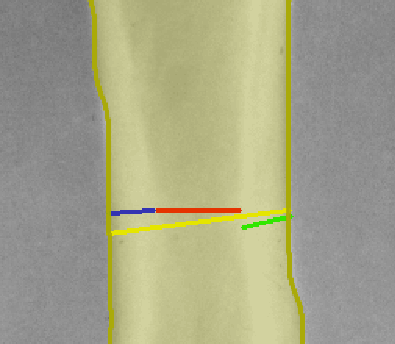
\includegraphics[width=.5\textwidth]{obrazky-figures/measures_comparision.pdf}
    \caption{\textbf{Measurement comparison.} Image depicts difference in measurement of~three separate regions and the full width of the bone.}
    \label{measures-comparision}
\end{figure}



%%%%%%%%%%%%%%%%%%%%%%%%%%%%%%%%%%%%%%%%%%%%%%%%%%%%%%%%%%%%%%%%%%%%%%%%%%%%%%%%%%%%%%%%%%%%%%%%%%%%%%%%%%%%

\section{Usage of the Algorithm}
\label{implementation}
The algorithm is executable as a terminal application, which therefore does not have any GUI elements. This can act as a certain disadvantage for the usability of the application itself. However, from the usability point of view and the perspective of resulting data collection, the GUI elements are not very indispensable and could serve more as a possible improvement to a potential extension of the application for greater user comfort.

The program was developed by Python version 3.8.5 in the Linux environment maintained under the Archlinux distribution. The primary libraries used in this work are Detectron2 and OpenCV version 4.5.1, which are used to work with images. Most of the source files in~the~\texttt{Modules} directory contain a PYX extension, which is an extension of the PY extension, and is used to recompile source files using C language for hardware optimization, which is discussed in more detail in the section \ref{hw-optimization}.

\subsection{Directory Structure}
The program has a directory structure, which consists of several scripts and other files. The~directory structure of the program is as follows:
\vspace{1mm}
\dirtree{%
.1 X-ray\textunderscore Detector.
.2 Annotations\textunderscore JSON.
.3 Metacarpals\textunderscore Train.json.
.3 ROI\textunderscore Train.json.
.2 doc.
.3 Doxyfile.
.3 manual.pdf.
.3 latex.
.3 html.
.2 README.md.
.2 Models.
.3 metacarpal\textunderscore model.pth.
.3 ROI\textunderscore model.pth.
.2 ROI\textunderscore Train.
.2 META\textunderscore Train.
.2 Utils.
.3 labelme2coco.py.
.2 clear.sh.
.2 install.sh.
.2 run.py.
.2 src.
.3 main.py.
.3 setup.py.
.3 Modules.
.4 canny.py.
.4 config.py.
.4 contour\textunderscore coordinates.pyx.
.4 distance.pyx.
.4 mask.pyx.
.4 roi.py.
.4 test.pyx.
.4 three\textunderscore regions.pyx.
.4 train.py.
}

The \texttt{Annotations\textunderscore JSON} directory contains appropriately validated JSON COCO annotations that were made using the \texttt{labelme2coco.py} script. The folder \texttt{doc} contains PDF manual documentation for the entire source code, generated using Doxygen tool. Folder also has documentation configuration file \texttt{Doxyfile}. This folder also contains \texttt{html} and \texttt{latex} subdirectories with autogenerated documentation sources like TEX and HTML files. Program has also brief installation and functionality manual described in file \texttt{README.md}. The \texttt {Models} directory is made up of trained models using the Detectron2 library, which is used for prediction in the X-ray image database. The \texttt {ROI\textunderscore Train} and \texttt {META\textunderscore Train} directories consist of annotated images to create a model with the appropriate JSON files generated by the LabelMe annotation application. The \texttt {Utils} directory contains the downloaded \texttt {labelme2coco.py} script, the meaning of which has already been described. The~\texttt{clear.sh} script deletes the generated shared objects (.so) of the library, which are created by recompiling modules with the PYX extension. The \texttt {install.sh} script downloads all the~necessary libraries and dependencies that are necessary to run the program. The \texttt{src} directory contains all the important source files of the program. The \texttt {setup.py} script is used to generate shared object libraries and C files for precompilation. The script \texttt {main.py} is the main module, the execution of which starts the algorithm. The \texttt {Modules} directory contains the scripts that are the core of the program. Finally, there is an executable script \texttt {run.py}, which starts the program.

\subsection{Program Running Options}
The program can be run relatively easily and it is possible to use several options for easier manipulation. These options can be combined between each other. If there are not used any of the optional flags, then the program processes dataset whose name is \textit{hardcoded} in the source code. The overview of use is as follows:

\begin{itemize}
    \item python \textbf{run.py}
    \item python \textbf{run.py -n} name of the image from where the program should start
    \item python \textbf{run.py -i} input image dataset directory path
    \item python \textbf{run.py -o} program output directory path
\end{itemize}

%%%%%%%%%%%%%%%%%%%%%%%%%%%%%%%%%%%%%%%%%%%%%%%%%%%%%%%%%%%%%%%%%%%%%%%%%%%%%%%%%%%%%%%%%%%%%%%%%%%%%%%%%%%%

\chapter{Testing on Given Database}
\label{testing}
This chapter describes the measurement outputs and focuses mainly on algorithm deficiencies and incorrect outputs. It also statistically compares the success of the algorithm on~the~dataset, the speed of image processing and possible hardware optimization, which will allow faster processing of the database.

\section{Used Database}
The used database, provided by Masaryk University from the Department of Anthropology, follows on from the Wrocław study \cite{wroclaw}. The \textit{Material and methods} section in this study further describes the origin of the data, and what number of samples of men and women were examined in this work. The provided database contains a total of 4862 X-ray images, where the images of women's hands are 2329 and the male hands represent the number of~2533. The X-ray images were made mainly for the left hand, but there are cases where both hands were taken on one image.

\section{Measurement of the Bone Full Width}
The following table \ref{table:full-width} shows the measurement success, including mask detection for the~whole width of the third metacarpal bone. If the mask detection is not correct, the~bone width measurement will not be correct either.

The table consists of the following parameters, which are expressed by abbreviations. \textit{G}~means gender, \textit{FD} is faulty detection and vice versa \textit{CD} is correct detection.

\begin{table}[ht]
    \centering
    \vspace{1mm}
     \begin{tabular}{V{2.5}c|c|c|c|cV{2.5}}
        \hlineB{2.5}
        \rowcolor{LightGray}
        \textbf{G} & \textbf{FD} & \textbf{FD(\%)} & \textbf{CD} & \textbf{CD(\%)}\\ \hlineB{2.5}
        Males & 0 & 0 & 2506 & 100 \\ \hline
        Females & 2 & 0.08343 &  2395 & 99.91657 \\ \hline
        Both & 2 & 0.0408 & 4901 & 99.9592 \\ \hline
    \end{tabular}
    \caption{Full width measurement comparison.}
    \label{table:full-width}
\end{table}

\section{Measurement of the Three Separate Bone Regions}
As in the previous part, this section will describe the accuracy of the measurement, which this time will concern the~extension of~the~algorithm with three separate regions of the~bone.

The \ref{table:three-regions} table shows the success of detection and measurement and contains abbreviations that are meaningfully identical to the previous section. The table contains one additional parameter, which describes the total measurement deviation if the bone was measured using two points across the width compared to three separate regions. Abbreviation \textit{WD} stands for width deviation. This deviation was calculated as follows:

\begin{align} 
  y &= \sum_{n=1}^{k} x - (a + b + c)\\
  d &= \frac{y}{k}
\end{align}

Variable \textit{d} is the total deviation, \textit{a}, \textit{b} and \textit{c} are the individual distances of three separate regions, i.e. left compact, medullary cavity and right compact. The variable \textit{x} is the~measured distance of a bone for its entire width. The \textit{k} variable is the number of detected bones. The~resulting value of \textit{y} is the total sum of the difference in distance between the~total bone width and the sum of the distances of the three regions. The resulting deviation is finally calculated by dividing the resulting sum and the total number of bones detected.

\begin{table}[ht]
    \centering
    \vspace{1mm}
     \begin{tabular}{V{2.5}c|c|c|c|c|cV{2.5}}
        \hlineB{2.5}
        \rowcolor{LightGray}
        \textbf{G} & \textbf{FD} & \textbf{FD(\%)} & \textbf{CD} & \textbf{CD(\%)} & \textbf{WD(mm)}\\ \hlineB{2.5}
        Males & 10 & 0.399 & 2496 & 99.601 & 0.1736 \\ \hline
        Females & 57 & 2.3779 & 2340 & 97.6221 & 0.1850 \\ \hline
        Both & 67 & 1.3665 & 4836 & 98.6335 & 0.1791 \\ \hline
    \end{tabular}
    \caption{The table of three regions measurement comparison.}
    \label{table:three-regions}
\end{table}

\section{Issues of the Created Algorithm}
Like many algorithms, this one is not error-free, and there are certainly a number of optimizations for processing speed, mask detection accuracy, and measurement accuracy. One of the major shortcomings of this algorithm is the mask prediction. The problem that caused the failure of traditional methods in image segmentation was the bone overlap. For~instance, in the image \ref{wrong-width} can be seen that the algorithm can very reasonably predict the~mask of~overlapping objects, which is the merit of the library Detectron2, which works with the method of instance segmentation. Nevertheless, the predicted mask is often imperfect and fails to accurately outline the boundaries of the bone itself. The image  \ref{contour-imperfection} shows how many parts of the mask are predicted to be inaccurate. The problem usually arises around the head of the bone, where this segmentation fails the most. Another inaccuracy in this mask is its \textit{waviness}, which is clearly visible in the image \ref{contour-imperfection} on the right side or at~the~top of the bone. The way to eliminate such problem is not entirely clear, but there is a~high probability that an improvement could be accomplished by a new model, which would be created using a large amount of annotated data. The most accurate model was created using training annotated data, the amount of which was 180, which is probably not enough to create a reliable model. Since the Department of Anthropology was notified of~such an inaccuracy, which is also reflected in the resulting file of coordinates, their initiative was shown through the annotation of images, because~the~annotation of professional material requires a lot of time and effort. After the~final communication, however, the conclusion was made, that the resulting contour is usable and will most likely find its application as stated by the Institute of Anthropology, such as the calculation of angles between the axes of bone and alike.

The second significant, although statistically negligible problem is the inaccurate prediction of all three regions while measuring individual bone widths. This problem arises again in~the~part of using the Detectron2 library, and it will probably be mainly related to~the~created model and the number of annotated images that were used to create this model (165 images). However, the images were made only after the creation of the basic part of~the~algorithm, which was able to measure the width of the whole bone. Using this width, it~was then possible to create an ROI, which automated the cutting out of~the~important part of~the~bone. As can be seen in the figure \ref{wrong-width}, the bone width for the left compact and the~medullary cavity was detected successfully, and thus the measurements could be performed on these two segments. As for the right compact, the mask was not detected, and thus it was not possible to measure this segment. Statistically, these problems occur in~percentage, which have been described in more detail in the table \ref{table:three-regions}.

The program therefore has two marginal problems, where the need to annotate a larger amount of data should be a critical point, and at the same time it should be the primary step in the future to improve this work.

\begin{figure}[!ht]
    \centering
    \begin{subfigure}[b]{.442\textwidth}
    \centering
       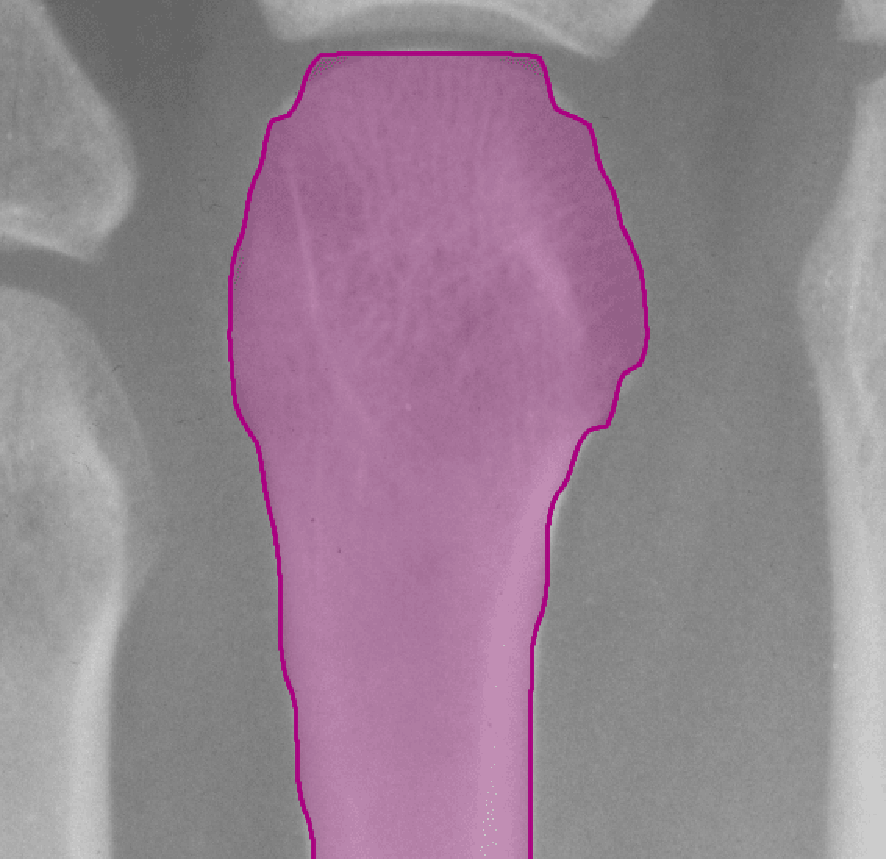
\includegraphics[width=\textwidth]{obrazky-figures/imperfection.pdf}
        \caption{}\label{contour-imperfection}
    \end{subfigure}
    \begin{subfigure}[b]{.3\textwidth}
    \centering
       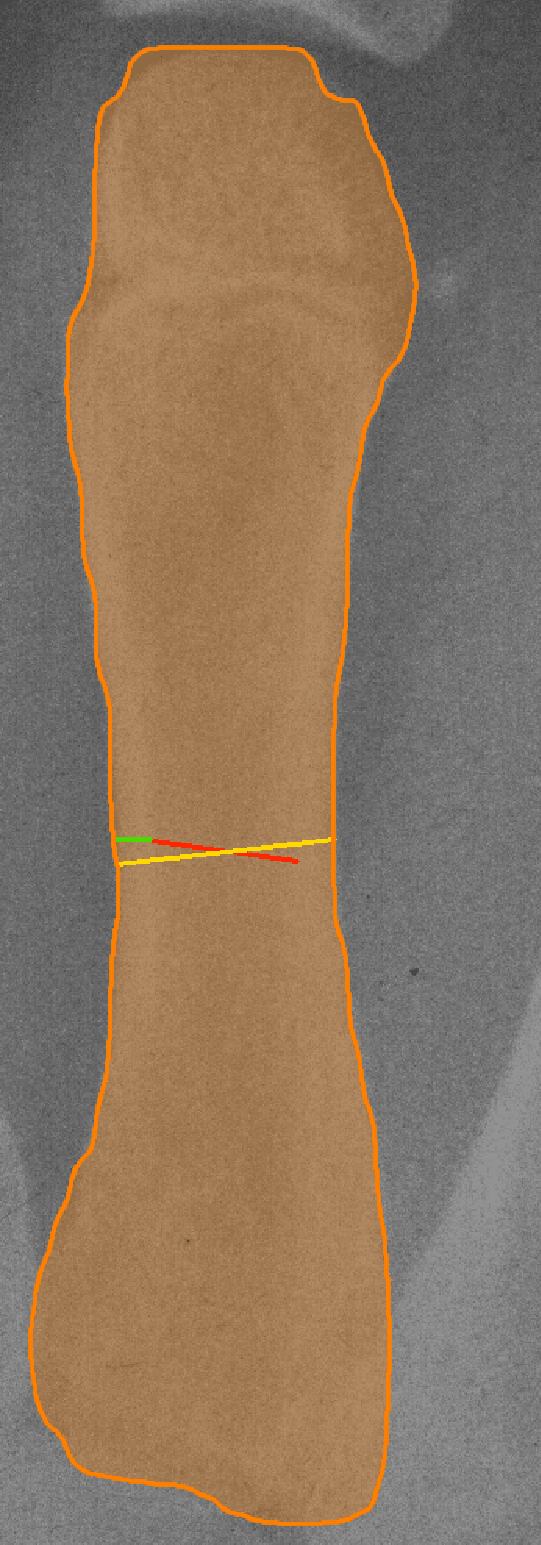
\includegraphics[width=.8\textwidth]{obrazky-figures/wrong_width.pdf}
        \caption{}\label{wrong-width}
    \end{subfigure}
    \caption{\textbf{Algorithm issues images.} (a) Detectron2 image mask prediction. (b) Binary mask of predicted image.}
    \label{algorithm-issues}
\end{figure}


\subsection{C Language Optimization}
\label{hw-optimization}
There are several different approaches on optimizing speed of the  algorithm, specifically written in Python. This algorithm uses the Cython \cite{cython} library, which can be used to~define, for example, the types of variables, as it is common in compiled languages. Cython generates shared object libraries and practically compiles Python into C. This optimization is chosen in this work mainly due to slow iterations in Python, where it is necessary to iterate several times through the image matrix.


\section{Computation Time per Image}
Usage of optimization in C language is possible to speed up the computation time by 40 seconds per one processed image which presents a significant difference. The measured time for processing was approximated and therefore is not always the precise number as stated in the table \ref{table:three-regions-time}.


\begin{table}[ht]
    \centering
    \vspace{1mm}
     \begin{tabular}{V{2.5}c|cV{2.5}}
        \hlineB{2.5}
        \rowcolor{LightGray}
        \textbf{Time per image without optimization} & \textbf{Time per image with optimization}\\ \hlineB{2.5}
        60s per image & 20s per image \\ \hline
    \end{tabular}
    \caption{Time comparison of one image processing without and with optimization.}
    \label{table:three-regions-time}
\end{table}

\section{Hardware Resources of Testing Device}
The overall processing of the database, besides creating models by the training process, took place on a machine with the following parameters:

\begin{itemize}
    \item CPU: \textbf{Intel® Core™ i5-8250U CPU @ 1.60GHz × 8}
    \item GPU: \textbf{Mesa Intel® UHD Graphics 620 (KBL GT2)} but no GPU utilization could be used due to incompatibility with Detectron2 library (Detectron2 is constructed using PyTorch\footnote{\url{https://pytorch.org/}} that only supports CUDA Nvidia)
    \item RAM: \textbf{11.5 GiB}
    \
\end{itemize}


\section{Comparison with Manual Measurements}
A sample of manual measurements performed by the Institute of Anthropology in selected 39 figures was used to evaluate the accuracy of measurements. From this sample, the average deviation between manual and automated measurements was calculated. The resulting deviation is on average \textbf{0.363572} millimeters, where the measured distances by automated method are mostly smaller than manual measurements, which can be caused by the imprecision of the detected contour. This may cause occasional inaccuracy in drawing the edges of the bone. The resulting measurement is included in the appendix \ref{appendix:a} in table \ref{table:comaprison}.

The table \ref{table:comaprison-three} compares the results of manual measurements with automated ones, where automated measurements represent the total sum of distances for measured three separate parts of bone, and thus left compact, right compact and meduallery cavity. The total value of the deviation in this case is \textbf{0.520193} millimeters. 


\chapter{Conclusion}
\label{conclusion}
The role of this work could be divided into two large parts. The first task was to create an~algorithm that will be able to detect the contour of the third metacarpal bone of the X-ray images available from the database provided by the anthropological institute. The second part, which the algorithm is designed to solve, is to measure the width of this detected bone in its narrowest diameter. Although a variety of types of images are not uniform, it was also necessary to find a solution that would be applicable to different-quality X-ray images containing a scanned hand.

For the introduction, it was necessary to get acquainted with the structure of metacarpal bone itself, including more specific terms such as compact of the bone, epiphysis, medullary cavity etc. Moreover, it was necessary to examine a certain sample of images in detail and identify the most significant problem for detecting bone contour. The marginal problem was the major overlap of metacarpal bones with each other, due to which it is often very difficult for the naked eye to determine exactly where the bone is located. On account of~this problem, it was necessary to examine the current state of the art for pattern recognition and object detection in the computer vision department. This has seen several approaches and methods, of which object detection using Mask R-CNN for instance segmentation is the most appropriate and accurate. The Detectron2 library was used for this detection, with the help of which it is possible to use convolutional neural networks for various types of image segmentation. Using this method, it was possible to predict the mask of the third metacarpal bone, which is a key moment for the development of this work. Based on this mask, it was possible to create the resulting contour of the bone using traditional methods and obtain its coordinates for expert analysis of the staff of Masaryk University.

The second part, which deals with the analytical measurement of the bone width, was implemented practically without the use of any higher abstraction, which is provided by any of the available libraries in the Python language. Classic iterations are used through an array of images, which consist of pixels, and an individual comparison of the distance between these pixels.

The algorithm itself, in addition to the basic distance measurement for the whole width of~the metacarpal bone, is extended by a functionality that allows measuring the bone width for three individual parts of the bone. These parts are the left and right compact bone, which are characterized by a light color in X-ray images. The third part is the medullary cavity, which forms the inside of the bone and its color is mostly darker. Detection of these three parts is re-mediated using the Detectron2 library and the instance segmentation method is used.

The created algorithm will help the Department of Anthropology to measure metacarpal bones automatically, thanks to which they will be able to analyze the change of~the~bone width during the growth of individuals and investigate genetic anomalies, or to detect various adverse growth factors. Another useful element may be that they will be able to avoid manual measurements, which in most cases happens only for the length of the bone and also speeds up the observation process in some way.

Like many working algorithms, in this case it would be also possible to improve the functionality itself in some way. One of the fundamental steps for improvement would be to~increase the accuracy of the predicted mask and thus to improve the resulting contour, which is often not completely precise and does not represent the exact shape of the bone. This step would also improve the measurement results, which are highly dependent on~the~detection of the~mask. It would also be possible to improve the analytical approach for measuring three bone segments, where it would be appropriate for the resulting distance for each segment to form one imaginary solid line, as in the case of measuring the total bone width. Last of~the possible improvement and extension for this algorithm would be the application for all the metacarpal bones in the hand. This extension was also considered to be quite useful, but at the same time the realization is not easy and requires a lot of time mainly due to~time-consuming manual image annotations. This issue should be taken into consideration for the future work.

%=========================================================================